% This is "sig-alternate.tex" V2.0 May 2012
% This file should be compiled with V2.5 of "sig-alternate.cls" May 2012
%
% This example file demonstrates the use of the 'sig-alternate.cls'
% V2.5 LaTeX2e document class file. It is for those submitting
% articles to ACM Conference Proceedings WHO DO NOT WISH TO
% STRICTLY ADHERE TO THE SIGS (PUBS-BOARD-ENDORSED) STYLE.
% The 'sig-alternate.cls' file will produce a similar-looking,
% albeit, 'tighter' paper resulting in, invariably, fewer pages.
%
% ----------------------------------------------------------------------------------------------------------------
% This .tex file (and associated .cls V2.5) produces:
%       1) The Permission Statement
%       2) The Conference (location) Info information
%       3) The Copyright Line with ACM data
%       4) NO page numbers
%
% as against the acm_proc_article-sp.cls file which
% DOES NOT produce 1) thru' 3) above.
%
% Using 'sig-alternate.cls' you have control, however, from within
% the source .tex file, over both the CopyrightYear
% (defaulted to 200X) and the ACM Copyright Data
% (defaulted to X-XXXXX-XX-X/XX/XX).
% e.g.
% \CopyrightYear{2007} will cause 2007 to appear in the copyright line.
% \crdata{0-12345-67-8/90/12} will cause 0-12345-67-8/90/12 to appear in the copyright line.
%
% ---------------------------------------------------------------------------------------------------------------
% This .tex source is an example which *does* use
% the .bib file (from which the .bbl file % is produced).
% REMEMBER HOWEVER: After having produced the .bbl file,
% and prior to final submission, you *NEED* to 'insert'
% your .bbl file into your source .tex file so as to provide
% ONE 'self-contained' source file.
%
% ================= IF YOU HAVE QUESTIONS =======================
% Questions regarding the SIGS styles, SIGS policies and
% procedures, Conferences etc. should be sent to
% Adrienne Griscti (griscti@acm.org)
%
% Technical questions _only_ to
% Gerald Murray (murray@hq.acm.org)
% ===============================================================
%
% For tracking purposes - this is V2.0 - May 2012

\documentclass{sig-alternate}

\usepackage{times}
\usepackage{helvet}
\usepackage{courier}

\usepackage{amsmath,amsfonts,amssymb}%,amsthm}
\usepackage{array}
\usepackage{amsmath,amssymb}
\usepackage[lofdepth,lotdepth]{subfig}
\usepackage{graphicx}
\usepackage{epstopdf}
\usepackage{color}
\usepackage[pdftex]{hyperref}

%\usepackage{hyperref}
\frenchspacing

\newcommand{\link}{\mathit{link}}
\newcommand{\post}{\mathit{post}}
\newcommand{\photo}{\mathit{photo}}
\newcommand{\video}{\mathit{video}}
\newcommand{\like}{\mathit{like}}
\newcommand{\ttag}{\mathit{tag}}
\newcommand{\comment}{\mathit{comment}}
\newcommand{\incoming}{\mathit{incoming}}
\newcommand{\outgoing}{\mathit{outgoing}}
\newcommand{\all}{\mathit{all}}
\newcommand{\app}{\mathit{app}}

% place holder spacing hacks
\newcommand{\secmoveup}{\vspace{-1.2mm}}                %{\vspace{-0.12in}}
\newcommand{\bigsecmoveup}{\secmoveup\vspace{-.0mm}}   %{\vspace{-0.08in}}

\newcommand{\textmoveup}{\vspace{-0mm}}               %{\vspace{-0.08in}}
\newcommand{\bigtextmoveup}{\textmoveup\vspace{-0.0in}} %{\vspace{-0.06in}}
\newcommand{\itemmoveup}{\vspace{-0mm}}              %{\vspace{-0.04in}}
\newcommand{\eqmoveup}{\vspace{-0.0in}}                 %{\vspace{-0.16in}}
\newcommand{\captionmoveup}{\eqmoveup\vspace{-0.0in}}   %{\vspace{-0.16in}}
\newcommand{\refitemmoveup}{\vspace{-0mm}}            %{\vspace{-0.16in}}
% hold but hide chunks of text
\newcommand{\eat}[1]{}
\newcommand{\yum}{}
\newcommand{\TODO}[1]{ {\color{blue}{\bf TODO:~{#1}}} }
\newcommand{\surl}[1]{\urlstyle{same}\url{#1}}

%\newcommand{}{\mathit{}}
\newcommand{\x}{\mathbf{X}}
\newcommand{\dislike}{\mathit{dislike}}
\newcommand{\likes}{\mathit{likes}}
\newcommand{\true}{\mathit{true}}
\newcommand{\false}{\mathit{false}}
\def\argmax{\operatornamewithlimits{arg\,max}}
\def\argmin{\operatornamewithlimits{arg\,min}}

\begin{document}
%
% --- Author Metadata here ---
\conferenceinfo{CIKM}{'13 San Francisco, USA}
%\CopyrightYear{2007} % Allows default copyright year (20XX) to be over-ridden - IF NEED BE.
%\crdata{0-12345-67-8/90/01}  % Allows default copyright data (0-89791-88-6/97/05) to be over-ridden - IF NEED BE.
% --- End of Author Metadata ---

\title{Social Affinity Filtering: Recommendation through \\Fine-grained Analysis of User Interactions and Activities}

\numberofauthors{1} %  in this sample file, there are a *total*
% of EIGHT authors. SIX appear on the 'first-page' (for formatting
% reasons) and the remaining two appear in the \additionalauthors section.
%
\author{
\alignauthor
Anonymous
%\alignauthor
%Ben Trovato\titlenote{Dr.~Trovato insisted his name be first.}\\
%       \affaddr{Institute for Clarity in Documentation}\\
%       \affaddr{1932 Wallamaloo Lane}\\
%       \affaddr{Wallamaloo, New Zealand}\\
%       \email{trovato@corporation.com}
%\alignauthor
%G.K.M. Tobin\titlenote{The secretary disavows
%any knowledge of this author's actions.}\\
%       \affaddr{Institute for Clarity in Documentation}\\
%       \affaddr{P.O. Box 1212}\\
%       \affaddr{Dublin, Ohio 43017-6221}\\
%       \email{webmaster@marysville-ohio.com}
%\alignauthor Lars Th{\o}rv{\"a}ld\titlenote{This author is the
%one who did all the really hard work.}\\
%       \affaddr{The Th{\o}rv{\"a}ld Group}\\
%       \affaddr{1 Th{\o}rv{\"a}ld Circle}\\
%       \affaddr{Hekla, Iceland}\\
%       \email{larst@affiliation.org}
%\and  % use '\and' if you need 'another row' of author names
%\alignauthor Lawrence P. Leipuner\\
%       \affaddr{Brookhaven Laboratories}\\
%       \affaddr{Brookhaven National Lab}\\
%       \affaddr{P.O. Box 5000}\\
%       \email{lleipuner@researchlabs.org}
%\alignauthor Sean Fogarty\\
%       \affaddr{NASA Ames Research Center}\\
%       \affaddr{Moffett Field}\\
%       \affaddr{California 94035}\\
%       \email{fogartys@amesres.org}
%\alignauthor Charles Palmer\\
%       \affaddr{Palmer Research Laboratories}\\
%       \affaddr{8600 Datapoint Drive}\\
%       \affaddr{San Antonio, Texas 78229}\\
%       \email{cpalmer@prl.com}
}

% There's nothing stopping you putting the seventh, eighth, etc.
% author on the opening page (as the 'third row') but we ask,
% for aesthetic reasons that you place these 'additional authors'
% in the \additional authors block, viz.

%\additionalauthors{Additional authors: John Smith (The Th{\o}rv{\"a}ld Group,
%email: {\texttt{jsmith@affiliation.org}}) and Julius P.~Kumquat
%(The Kumquat Consortium, email: {\texttt{jpkumquat@consortium.net}}).}

%\date{30 July 1999}

% Just remember to make sure that the TOTAL number of authors
% is the number that will appear on the first page PLUS the
% number that will appear in the \additionalauthors section.

\maketitle
\begin{abstract}
%%
%% Template abstract.tex
%%

\chapter*{Abstract}
\label{cha:abstract}
\addcontentsline{toc}{chapter}{Abstract}

Social networks such as Facebook allow users to create a rich and verbose profile composed of both user specific interactions (such as 
comment and message passing, tags, likes, etc) and user preferences (such as favourite movies and music, group memberships, page likes, etc). 
These interactions and preferences define implicit groups having varying affinities to the preferences of a given user; 
these affinities can be learned from data and then leveraged to predict a user's own preferences, e.g., 
whether a user will "like" a certain news article or blog post.

The objective of this thesis is to decipher which of these aforementioned affinity measures are truly predictive of a user's like preferences.

The success of our predictions are evaluated using the machine learning algorithms of  
\emph{Naive Bayes}, \emph{Logistic Regression} and \emph{Support Vector Machines}, and the results are compared to previous 
work using the state of the art social collaborative filtering technique of \emph{Social Matchbox} as a baseline. 
The data is sourced from a set of over 100 Facebook users and their interactions with over 39,000 friends during a four month period.

Our analysis has shown that user interactions in themselves are not highly predictive of user likes, however user preferences are. 
This increasingly predictive trend continues as we limit user exposure (ensuring some $k$ number of users $u$ have liked a link $v$) over links. 
We conclude by analysing a combination of the most predictive user preference affinity measures, offer a summary of our work to date and propose 
recommendations for further research in this area.

%%% Local Variables: 
%%% mode: latex
%%% TeX-master: "thesis"
%%% End: 

\end{abstract}

% A category with the (minimum) three required fields
\category{H.3.3}{Information Search and Retrieval}{Information Filtering}
%A category including the fourth, optional field follows...
%\category{D.2.8}{Software Engineering}{Metrics}[complexity measures, performance measures]

%\terms{Theory}

\keywords{social networks, collaborative filtering, recommender systems}

\section{Introduction}

%!TEX root = document.tex

\label{sec:introduction}

% motivate socical recommendation 
Online social networks such as Facebook record a rich set of user
preferences (likes of links, posts, photos, videos), user traits,
interactions and activities (conversation streams, tagging, group
memberships, interests, personal history and demographic data).  This
presents myriad new dimensions to the recommendation problem by making
available a rich labeled graph structure of social interactions and
content from which user preferences can be learned and new
recommendations can be made.

Existing recommendation methods for social networks aggregate this
rich social information into a simple measure of user-to-user interaction 
that can be leveraged to model user homophily via social
regularization~\cite{lla,socinf,sr,rrmf, Noel2012NOF}, a trust
ensemble~\cite{ste}, or a low-rank factorization of the social
interactions matrix~\cite{sorec}.  But in aggregating all of these
interactions and common activities into a single strength of
interaction, we 
%show effectively that the signal present in this 
%information gets drowned out in the noise --- some fine-grained
%interactions and activities are highly informative, but most are not.
ask whether important preference information has been discarded?
Indeed, the point of departure for this work is the hypothesis that
different fine-grained interactions (e.g. commenting on a wall or
getting tagged in a video) and activities (e.g., being a member of a
university alumni group or a fan of a TV series) \emph{do} represent
different preferential {\em affinities} between users, and moreover
that effective {\em filtering} of this information (i.e., learning
which of these fine-grained interactions and activities are 
informative) will lead to improved accuracy in social recommendation.

%% No longer fits cleanly in the intro, should be moved into related
%% work is not already mentioned there.  -SPS
\eat{
In the context of recent work on social
recommendation~\cite{sorec,ste,lla} and information diffusion
~\cite{Goel2012structure,Romero2011hashtag,Bakshy2012chamber}, it is
important to know which of these interactions or common traits are
actually reflective of common preferences.}

To quantitatively validate our hypotheses and evaluate the
informativeness of different fine-grained features for social
recommendation, we have built a Facebook App to collect detailed user
interaction and activity history available through the Facebook Graph
API along with user preferences solicited by the App on a daily basis.
Specifically, each day our App recommends three links to each App user
that are collected from the timeline of other users (both friends and
non-friends) and we record users' explicit likes and dislikes of these
recommended links.  Given this data, we define \emph{social affinity
groups (SAGs)} of a target user (ego) as sets of surrogate users
(alters) serving as proxies for an ego's preferences; these SAGs are
defined according to fine-grained
\emph{interactions} (e.g., users who have been tagged in the target user's
video) and \emph{activities} (e.g., users who have liked the same
political party page that the target user has liked).  Given a set of
SAGS for a user, (1) we define a novel recommendation method called
{\em social affinity filtering (SAF)} where we learn to predict
whether a user will like an item based on the surrogate item
preferences of members of each SAG, and (2) we analyse the relative
informativeness of SAGs across a variety of dimensions such as type,
frequency of friend preferences, and activity membership size.

In the four months that our App was active, we collected data for a
set of Facebook app users and their full interactions with 38,000+
friends along with 22 distinct types of interaction and users activity
for 3000+ groups, 4000+ favourites, and 10,000+ pages.  In subsequent
sections that outline our experimental methodology and results in
detail, we make the following critical observations:
\begin{itemize}
\item We found that SAF significantly 
outperforms numerous state-of-the-art collaborative filtering and social recommender 
systems, by up to 6\% in accuracy using just \emph{page} (like) features.
Because the reluctance of a user to install an App increases with the number
of permissions requested, this suggests a state-of-the-art social recommendation App 
need only request permissions for a user's \emph{page} likes in order to achieve
state-of-the-art recommendation accuracy.
% -- in short, these fine-grained features can be very informative.
% Also, what about combining all features?  Not enough data?  -SPS
% Probably also much faster -- should we show a table of train and test times?  -SPS
\item We found that groups, pages, and favourites make for more informative
SAGs than those defined by user-to-user interactions.  This is likely because the former can be
applied to SAGs over the entire Facebook population 
rather than just a user's friends (where the data is considerably limited).
\item Among the interactions, we found that those on videos are more predictive than those on other content types (photos, post, link), and that outgoing interactions (performed by the ego on the alter's timeline) 
are more predictive than incoming ones (performed by alters on the
ego's timeline), although the level of exposure of an ego to an
alter's preferences is more important than the directionality of the
interaction with the alters.
% Below: not sure I quite understand ``persistent'' and ``temporally synchronized'' here... 
% are there better terms or can they be further (briefly) explained?  -SPS
\item %{\bf TODO: see Latex comments.} 
Among {\em groups}, {\em pages} and {\em favourites}, we found that only
a small subset of the features were actually informative, bringing into question the efficacy of 
previous social recommendation approaches that aggregate social information between
two users into a single numerical value.  We found that the most  
predictive activity SAGs tend to have small memberships.  We also found features
corresponding to ``long-tailed'' content (such as music and books)
can be much more predictive than those with fewer choices 
(e.g. interests or sports). 
 %to generic (such as interests) or activities that require 
 %simultaneous participation (such as sports) are less predictive of 
 %user interest than topics that are ongoing or persistent in time (such as TV, books).
\end{itemize}
As detailed in the subsequent sections, these findings not only
demonstrate the power of leveraging fine-grained interaction and
activity features but they also suggest which of these features can
be most informative when building state-of-the-art
SAF-based recommenders.
%  This
%latter point is quite important since as already noted, there is
%a trade-off between the number of permissions a Facebook App requests
%and user uptake.
%
%we note later -- the more
%permissions an App requests, the less likely a user is to grant
%permissions to the App, so choosing permissions (i.e., social
%features) well is crucial for achieving good recommendations with
%minimal intrusion into a user's privacy.

\eat{
To better understand these subtleties and to understand what
social interactions and user traits reflect common preferences on
Facebook, we proceed in the following sections to describe our data,
our experimental methodology, and various analyses according to our
methodology that shed light on the above questions. 
On one hand our observations confirm certain observations made previous 
on different networks, such as the diminishing returns of repeated exposures, 
on the other we also see a few new clues such as 
that very specific types of outgoing interactions are more predictive 
than other interactions. 
We then conclude with a summary of the key novel observations arising
from this study.
}

\yum



\section{Social Affinity Groups}
\label{sec:methodology}

The major objective of this paper is to evaluate the effectiveness of \textit{Social Affinity Filtering(SAF)} and fine grained 
analysis of the informativeness of Interactions and Activities.We divide our recommendation algorithm into two categories based 
on Interactions and Activities of target user's \textit{ Social Affinity Groups(SAG)} with target item, 
namely \textit{Interaction  Social Affinity Groups(ISAG)} and \textit{Activity Social Affinity Groups(ASAG)}.

\begin{itemize}
  \item \textbf{Interaction  Social Affinity Groups}: We define the set of interaction affinity classes based on 
  Interaction modality, action and direction as
  \begin{quote}
  \begin{math}
  	\textit{Interaction Affinity Classes} = \{link, post, photo, video\} \times \{like, tag, comment\} \times \{incoming, outgoing\}
  \end{math}
  \end{quote}
  %Additionally, we add friendship interaction affinity class. \\
  We define 
  \begin{quote}
  \textit{ISAG(u, i)} : set of the users who have interaction $i$ with user $u$.\\
   For example,\\
   \textit{ISAG(u, link-like-incoming)} : set of all users who have liked link posted by user $u$. \\
   \textit{ISAG(u, link-like-outgoing)} : set of all users whose link is liked by user $u$. \\
  \end{quote}
\item \textbf{Activity Social Affinity Groups}: We define activity affinity groups based on group membership, page likes and user favourites.
	\begin{quote}
	\textit{ASAG(u, i)} : set of the users who share entity $i$ (group, page, favourite) with user $u$.   
	\end{quote}
\end{itemize}
Finally, we define
\begin{quote}
\begin{math}
likes(u,i) =  \begin{Bmatrix}
	  True & \text{if user $u$ likes item $i$}\\
	  False & \text{otherwise}
	  \end{Bmatrix}
\end{math}
\end{quote}
\subsection{Social Affinity Features}
\begin{itemize}
  \item \textbf{Interaction Social Affinity Features} : We define Interaction affinity features for target user $u$ and item $i$ for 22 ISAG's classes 
  $ \langle X_{1},X_{2}\ldots,X_{k}\rangle$ as
  \begin{quote}
  \begin{math}
   X_{k,u,i} = \begin{Bmatrix}
   		True & if\ \exists\ v\in \ \ ISAG(u,k) \wedge likes(v,i)\\ \\
   		False & otherwise
   \end{Bmatrix}
  \end{math}
  \end{quote}
  Additionally we add friend feature which encodes whether the target item $i$ is liked by friend or not.
  \item \textbf{Activity Social Affinity Features} : We define activity affinity features for target user $u$ and item $i$   \
  $ \langle X_{1},X_{2}\ldots,X_{k}\rangle$ as\\ \\
  \begin{math}
   X_{k,u,i} = \begin{Bmatrix}
   		True & if\ \exists\ v\in \ ASAG(u,k) \wedge likes(v,i)\\ \\
   		False & otherwise
   \end{Bmatrix}
  \end{math}
	In our analysis we use only those features(groups, pages and favourites) that is joined/liked by atleast one of our app user.
\end{itemize}

With Affinity features defined, we use naive bayes, Logistic regression and Support Vector Machine (SVM) model to predict whether 
user likes the link or not. Logistic Regression and Support Vector Machine algorithm is implemented using LIBLINER \cite{liblinear}.

Acknowledging the fact that, in real world social recommendation task, activitiy features grows very quickly as number of user in social 
networks increase we explore informativeness of social affinity features from the recommender system standpoint. Furthermore, its compelling
to understand informativeness of the interaction features. For fine grained analysis of activities and interactions we rank the features using
\textit{Conditional Entropy} H(Y$|$X=true).

\textit{Conditional Entropy} is defined as
\begin{quote}
\begin{math}
H(Y|X=True) = \\-\sum_{y\in{(like,dislike)}} p(y|X$=$true)$ $log( p(y|X$=$true))
\end{math}
\end{quote}
 Conditional Entropy measures the extent of discriminitiveness of the features.\\

With the data and methodology now defined including all dimensions of our analysis, we now proceed to an in-depth discussion of our findings.





 






%!TEX root = document.tex

\section{Social Affinity filtering}

{\bf TODO: need to revise and describe features using uniform notation... Suvash used upper and I used lower case, need to follow Suvash's notation.}

%Social affinity filtering (SAF) is based on the idea that affinity
%between users expressed in social networks via interactions and
%activities is predictive of user preferences.  
Social affinity group and the associated features defined in Sec~\ref{ssec:SAfeature} 
are used to build predictors for $\likes(u,i)$ given features $X$.
%as follows: a classifier takes a user $u$ and item $i$ and must predict
%whether $\likes(u,i)$ given features that can be derived from the
%social network.  
In SAF, these features are the boolean
variables $X_{k,u,i}$ indicating whether any users in the $k$th SAG of
user $u$ also liked $i$.  For example, $k$ could be the SAG of $u$ for
the interaction of $\textit{link-like-incoming}$ or the activity of
liking the {\em Obama Re-Election Headquarters} Facebook page.  Then knowing whether
anyone in each SAG $k$ for user $u$ likes item $i$ provides a rich set
of fine-grained features for prediction.  It is up to SAF to learn how
to weight each SAG to aggregate their preferences into one final
prediction, which is done by training on historical data.

Formally, given a user $u$ and item $i$, a SAF classifier is a
function: $f: \x \to y$ where $y \in \{ \like, \dislike \}$ and $\x =
\langle u,i,x_1,\ldots,x_k \rangle$ where $x_j \in X_j$ ($1 \leq j
\leq k$) as previously formally defined in the Methodology.  To train $f$, one
simply provides a dataset of historical observations $D = \{ \langle
\x,y \rangle \}$, e.g., $f$ could be a linear classifier trained by an
SVM, logistic regression, or na\"{i}ve Bayes.  Then for future
predictions, we simply are given $\x$ and we ask the SAF classifier to
predict $y = f(\x)$.



\section{Evaluation}

\subsection{Data Description}
\label{sec:datadesc}
%!TEX root = document.tex

{\bf TODO: need to address all missing info in reviews and probably rewrite for clarity: what the app did, what suggestions it made to user, the fact that it was offline batch and not online, whether there was rank bias -- no, independent ratings.  Tables provide good summaries so should not need to be too verbose in this section.}

We built a Facebook App\footnote{Name and link omitted
for anonymity.} to collect information about users, 
their interactions and preferences on daily recommended links.  
%data about Facebook users and their Facebook friends
%are collected through our Facebook App. 
Our dataset contains information about each App user along with their
interactions with all of their friends.  The
data collection is performed with full permission from the user and in
accordance with an approved Ethics Protocol\footnote{Link omitted for
anonymity.}.

%% I'm going to let the table do the summarizing this time
\eat{
Over 119 users installed the Facebook App during the evaluation
period.\footnote{In order to collect full interactions among App users
as required in our experimentation, our App requested to collect
information posted to \emph{friends'} timelines.  With such expressive
permissions concerning friend interactions, most potential users were
hesitant to install the App hence after a one month user drive period
we were able to attract the pool of users used in the experiments.}
From these core App users, the App has access to their detailed
Facebook profiles and their interactions with a total of 38,259
friends.
}

%interaction data.  
While we have complete interaction data for the App users with their
friends, and profile data (including wall post data) for the App users
and friends, we do not have complete interactions for the App users'
friends (unless they themselves are App users).  Hence in the
forthcoming analysis, we limit our evaluation to App users for which
we are assured to have full interaction data.

Our App tracks app user's (and their friends') details and
interactions on Facebook.  Interactions that occur through wall posts
provide a rich variety of content and interaction data.  We
distinguish four Facebook items from wall posts: general posts (e.g.,
status updates, activity updates such as new friends), links, photos
and videos. Four main interactions on these items are permitted by
Facebook: posting an item to a friend's wall, commenting, liking, and
tagging. Furthermore, Facebook allows user to interact with entities
(groups, pages and favourites) via membership and liking. The app also
keep tracks of the information of user's group membership, page likes
and favourites.  The App does not track deletions of these items,
interactions (e.g., unlike) and memberships for performance reasons
and we found very few deletions during an initial testing stage.  We
summarize relevant basic statistics of the data in
Table~\ref{tab:interactions}-\ref{tab:likeinfo} below.
Table~\ref{tab:interactions} summarizes the number of records for each
item (row) and interaction (column)
combination. Table~\ref{tab:demographics} shows some demographics from
user profiles. Table \ref{tab:interests} shows the group membership,
page like and favourites counts for app users and all users.

Our app recommends links to users every day, where the users may give
their feedback on the links indicating whether they liked it or
disliked it. Users are recommended links that are collected either
from friends or non-friends. Throughout this paper, app user rated
link data is used to evaluate the recommendation algorithms.
Table \ref{tab:likeinfo} shows the statistics of the app user rating
for friend and non-friend recommendations.
      							
\begin{table}
\centering
\begin{tabular}{|>{\small}l|>{\small}r|>{\small}r|}
\hline
& \textbf{App Users} & \textbf{Ego network} \\
& & \textbf{of App Users} \\
\hline
Users & 119 & 38,378 \\
\hline
Male & 85 & 20,840 \\
\hline
Female & 33 & 17,032 \\
\hline
\end{tabular}
\caption{App user demographics}
\label{tab:demographics}
\end{table}

\begin{table}
\centering
\begin{tabular}{|>{\small}l|>{\small}r|>{\small}r|>{\small}r|}
\hline
\textbf{App Users} & \textbf{Tags} & \textbf{Comments} & \textbf{Likes} \\
\hline
\textbf{Post} & 7,711 & 22,388 & 15,999 \\
\hline
\textbf{Link}  & --- & 7,483 & 6,566 \\
\hline
\textbf{Photo} & 28,341 & 10,976 & 8,612 \\
\hline
\textbf{Video} & 2,525 & 1,970 & 843 \\
\hline
\hline
\textbf{Ego network} & \textbf{Tags} & \textbf{Comments} & \textbf{Likes} \\
\textbf{of App Users}  & & & \\
\hline
\textbf{Post} & 1,215,382 & 3,122,019 & 1,887,497 \\
\hline
\textbf{Link} & --- & 891,986 & 995,214 \\
\hline
\textbf{Photo} & 9,620,708 & 3,431,321 & 2,469,859 \\
\hline
\textbf{Video} & 904,604 & 486,677 & 332,619 \\
\hline
\end{tabular}
\caption{Statistics on user {\em Interactions}, grouped by item {\em Modality} and {\em Action type}.}
\label{tab:interactions}
\end{table}


\begin{table}[t!]
\centering
\begin{tabular}{|>{\small}l|>{\small}r|>{\small}r|}
\hline
& \textbf{App Users} & \textbf{Ego Network} \\
& & \textbf{of App Users} \\
\hline
Groups & 3,469 & 373,608 \\
\hline
Page Likes & 10,771 & 825,452 \\
\hline
Favourites & 4,284 & 892,820\\
\hline
\end{tabular}
\caption{Statistics on user {\em Actions}, counted for {\em groups, pages} and {\em favorites} over the App users and their ego network.}
\label{tab:interests}
\end{table}

\begin{table}[t!]
\centering
\begin{tabular}{|>{\small}l|>{\small}r|>{\small}r|}\hline
&\textbf{Friend}  & \textbf{Non-Friend} \\
&\textbf{recommendation}  & \textbf{recommendation} \\
\hline
Like& 1392 & 1127 \\
\hline
Dislike& 895 & 2111\\
\hline
\end{tabular}
\caption{Dataset breakdown of prediction target $like(u,i)$, by the source of the link (friend/non-friend) and value (true/false).}
\label{tab:likeinfo}
\end{table}


\eat{ %% suvash's original table
\begin{table}
\centering
\begin{tabular}{|>{\small}l|>{\small}r|>{\small}r|>{\small}r|>{\small}r|}
\hline
\textbf{App Users} & \textbf{Posts} & \textbf{Tags} & \textbf{Comments} & \textbf{Likes} \\
\hline
\textbf{Wall} & 36,359 & 7,711 & 22,388 & 15,999 \\
\hline
\textbf{Link} & 5,304 & --- & 7,483 & 6,566 \\
\hline
\textbf{Photo} & 4,933 & 28,341 & 10,976 & 8,612 \\
\hline
\textbf{Video} & 245 & 2,525 & 1,970 & 843 \\
\hline
\hline
\textbf{App Users} & \textbf{Posts} & \textbf{Tags} & \textbf{Comments} & \textbf{Likes} \\
\textbf{and Friends} & & & & \\
\hline
\textbf{Wall} & 4,301,306 & 1,215,382 & 3,122,019 & 1,887,497 \\
\hline
\textbf{Link} & 678,612 & --- & 891,986 & 995,214 \\
\hline
\textbf{Photo} & 1,268,816 & 9,620,708 & 3,431,321 & 2,469,859 \\
\hline
\textbf{Video} & 59,244 & 904,604 & 486,677 & 332,619 \\
\hline
\end{tabular}
\caption{The number of interactions Tables. Rows are type of Facebook item and columns are type of Facebook interaction.}
\label{tab:interactions}
\end{table}
}


\subsection{SAF Analysis}
\label{sec:saf_analysis}
In this section, we compare novel SAF-based methods with a
variety of (social) collaborative filtering baselines:
\begin{enumerate}
\item {\bf Most Likely Class Constant Predictor (Const)}
\item {\bf Nearest Neighbor (NN)}~\cite{bellkor}
\item {\bf Matrix Factorization (MF)}~\cite{pmf}
\item {\bf Social Matchbox (SMB)}~\cite{Noel2012NOF}
\end{enumerate}
Here, Const serves as a lower bound on performance, NN and MF are two
well-known state-of-the-art \emph{non-social} collaborative filtering
algorithms, and SMB is a state-of-the-art \emph{social} collaborative
filtering algorithm employing matrix factorization with social
regularisation.

Among the novel SAF methods, we analyse four different sets of 
social affinity features:
\begin{enumerate}
\item {\bf Interaction Social Affinity Features (ISAF)}
\item {\bf Activity-based Social Affinity Features (ASAF)} for 
  \begin{enumerate}
  \item {\bf Group Memberships}
  \item {\bf Page Likes}
  \item {\bf Favourites}
  \end{enumerate}
\end{enumerate}
Furthermore, for these four classes of features, we train
one of three classifier types, leading to the following
classes of SAF recommenders evaluated in our experiments:
\begin{enumerate}
  \item {\bf Na\"{i}ve Bayes (NB-ISAF, NB-ASAF)}
  \item {\bf Support Vector Machines (SVM-ISAF, SVM-ASAF)}
  \item {\bf Logistic Regression (LR-ISAF, LR-ASAF)}
\end{enumerate}
NB uses a standard Na\"{i}ve Bayes implementation, 
SVM and LR are both implemented using \textit{LIBLINEAR}~\cite{liblinear}.

In all experiments, we report average classification accuracy
(fraction of correct classifications in held-out test data) using
10-fold cross validation and provide standard error bars corresponding
to 95\% confidence intervals.
%#suvash#
%Accuracy is defined as  
%\begin{align*}
%accuracy = \frac{\#\ correct\ predictions}{\#\ predictions}
%\end{align*}

Fig~\ref{Fig1} compares the above baselines and SAF algorithms.  In
all of these experiments, SAF variants performed statistically
significantly better than the best baseline (SMB), except for NB-ASAF
which we conjecture is due to violation of feature independence
assumptions that become more pronounced as the number of features
increases (n.b., NB-ISAF uses 22 features while NB-ASAF uses 1000's of
features).

%%%%%%%%%%%%%%%%%%%%%%%%%%%%%%%%%%%%%%%%%%%%%%%%%%%%%%%%%%%%%%%%%%%%%%%%%%%
\begin{figure*}[tbh!]
%\centering
\hspace{-6mm}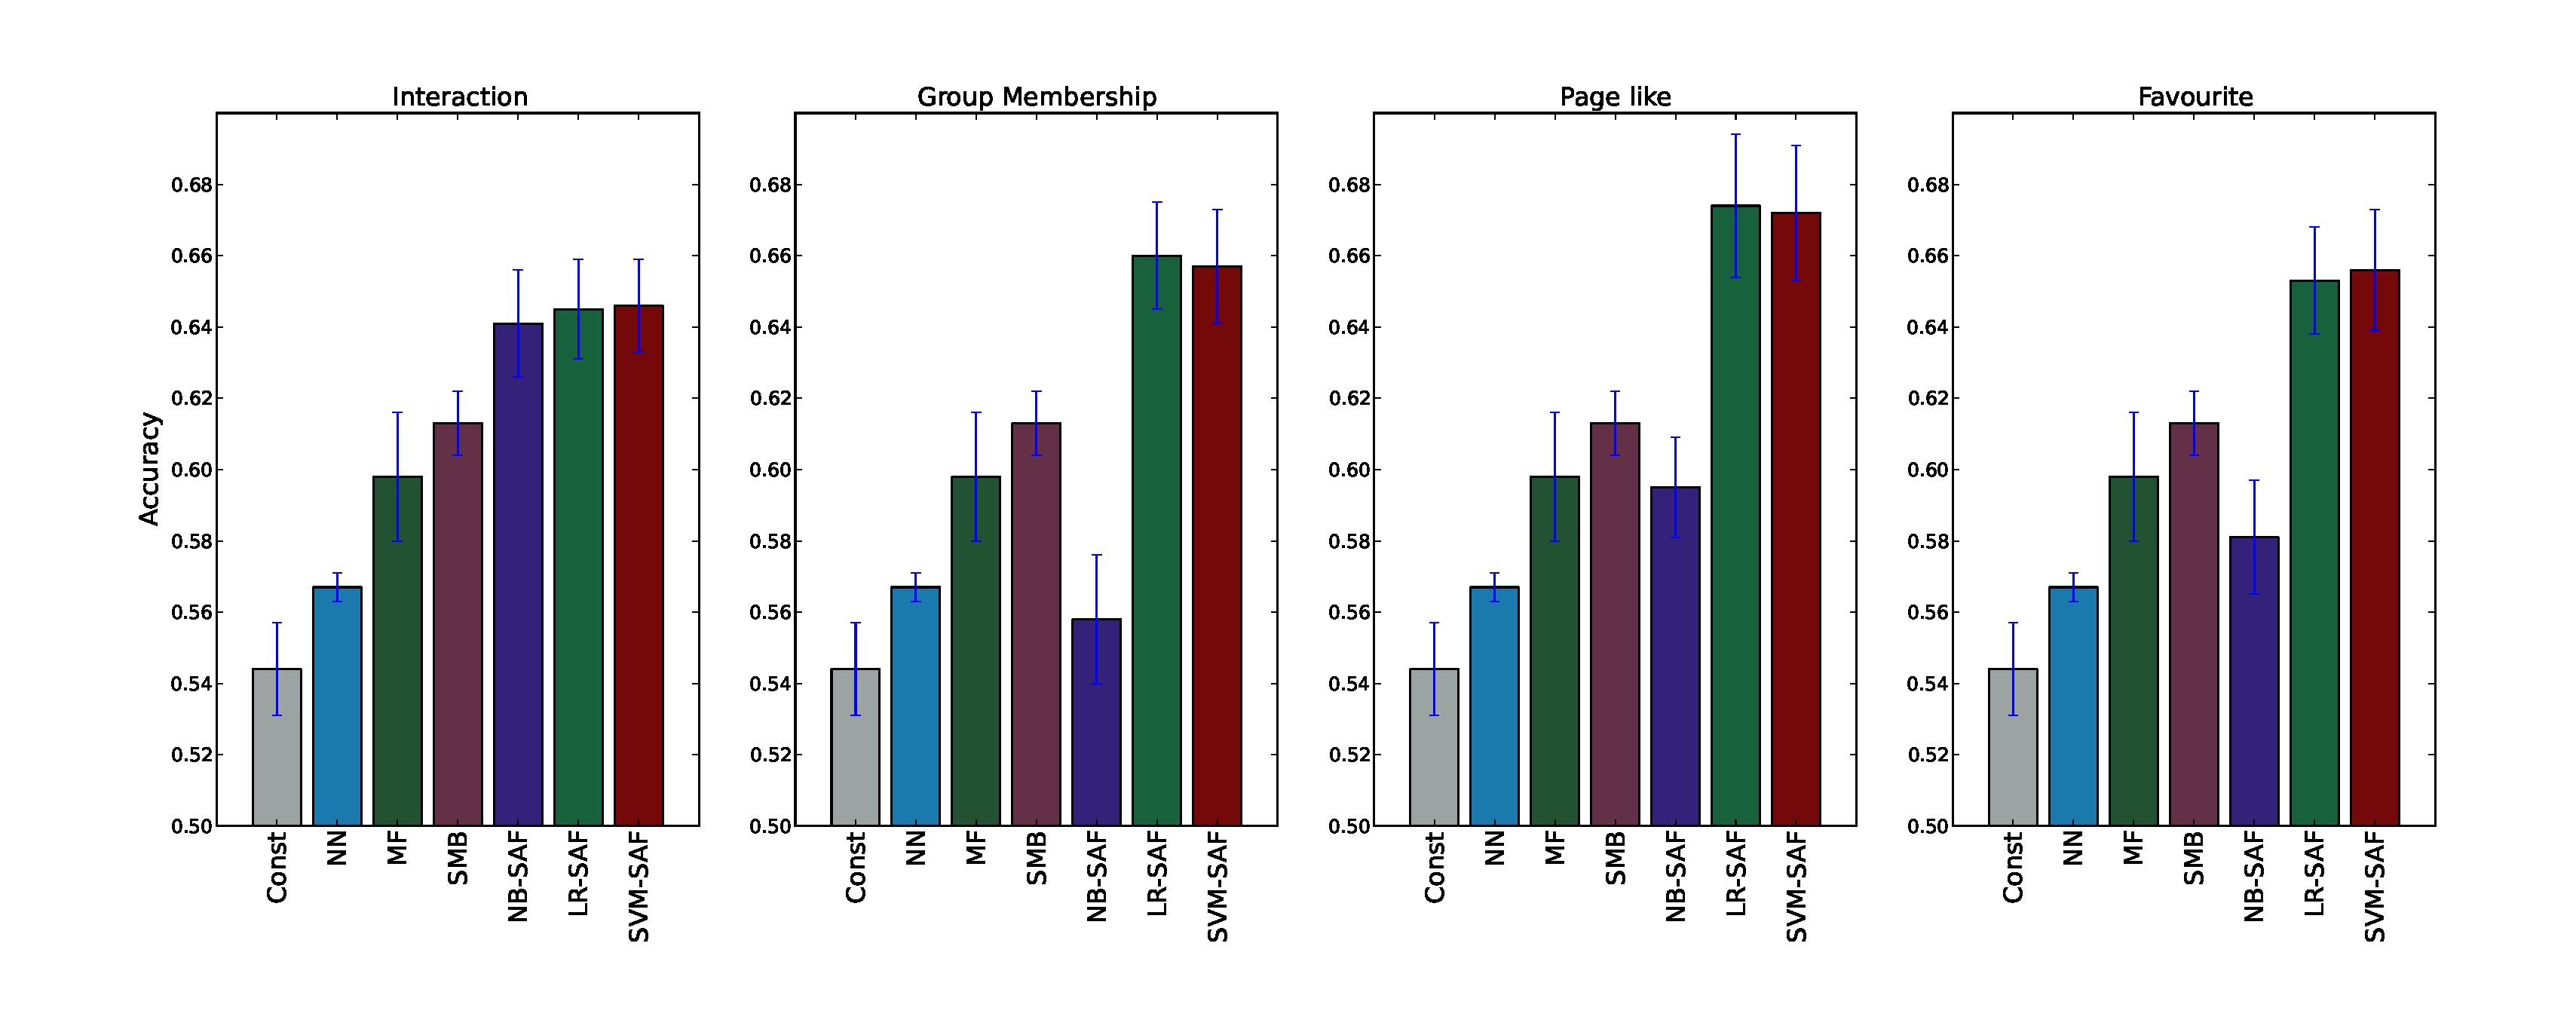
\includegraphics[height=80mm,width=190mm]{data/newPlots/accuracy.eps}
\vspace{-6mm}
\caption{Comparision of a simple baseline (Const), two collaborative
  filtering baselines (NN and MF), a social collaborative filtering
  baseline (SMB) and novel SAF recommenders using different feature
  sets (one ISAF and three ASAF sets) and classifiers (NB,LR,SVM).
  The best SAF-based model (LR-ASAF) --- for Page likes --- significantly outperforms
  all baselines by at least 6\%.  Combining all four feature sets (not shown)
  does not lead to improvement over Page likes features alone.}
\label{Fig1}
\end{figure*}
%%%%%%%%%%%%%%%%%%%%%%%%%%%%%%%%%%%%%%%%%%%%%%%%%%%%%%%%%%%%%%%%%%%%%%%%%%%

%%%%%%%%%%%%%%%%%%%%%%%%%%%%%%%%%%%%%%%%%%%%%%%%%%%%%%%%%%%%%%%%%%%%%%%%%
\begin{figure*}[tbh!]
\centering
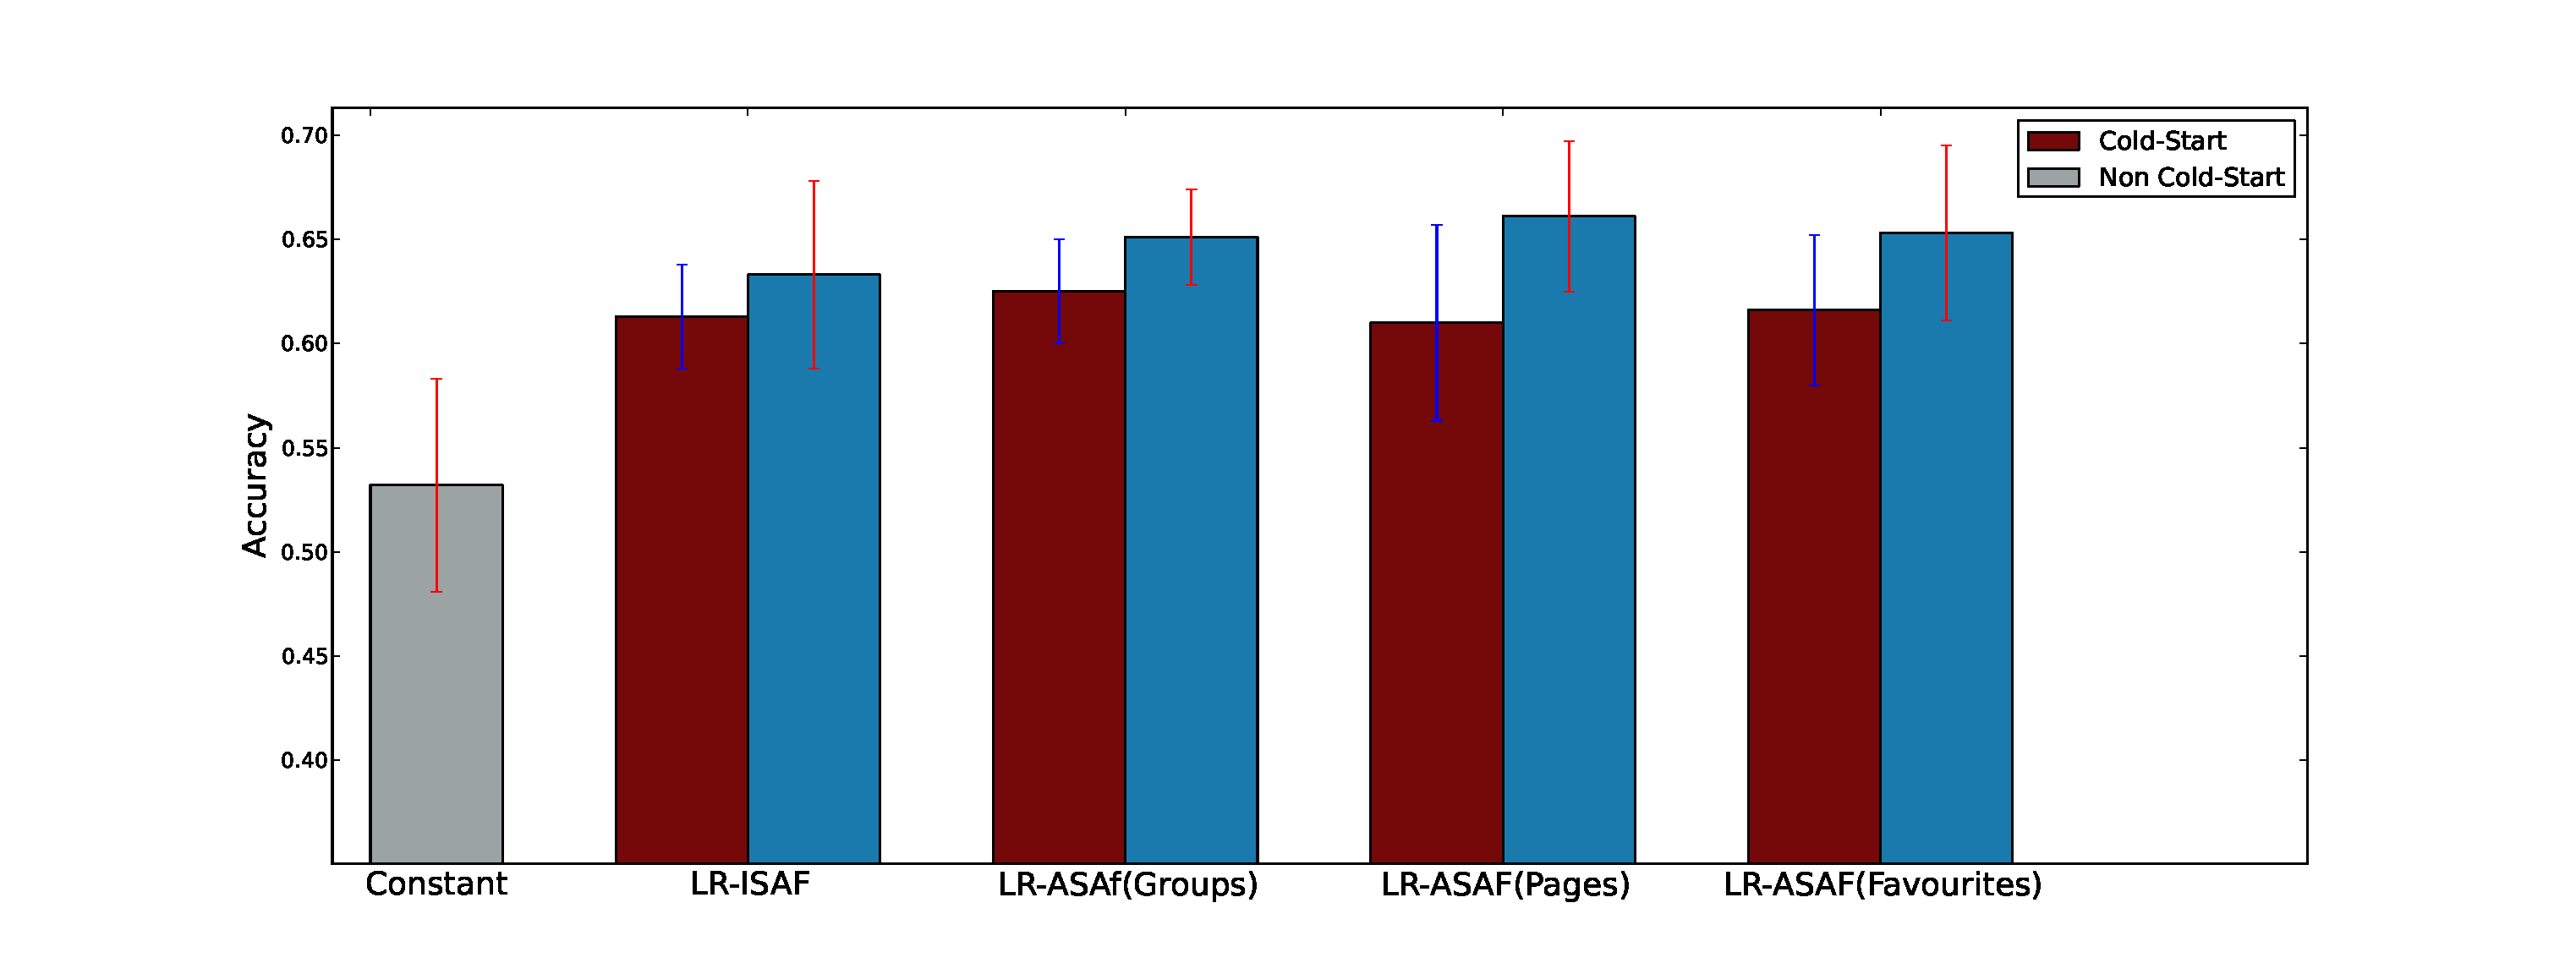
\includegraphics[width=180mm,height=50mm]{data/newPlots/cold_start.eps}
\vspace{-6mm}
\caption{Cold-start evaluation of SAF: accuracy evaluated on cold-start users 
  outperforms the most likely class (Constant) predictor baseline and is
  somewhat comparable to the non cold-start case when all test user data is \emph{not}
  withheld from training.}
\label{fig:coldstart}
\end{figure*}
%%%%%%%%%%%%%%%%%%%%%%%%%%%%%%%%%%%%%%%%%%%%%%%%%%%%%%%%%%%%%%%%%%%%%%%%%
 

In terms of the best recommenders, we observe that LR-ASAF and
SVM-ASAF perform comparably to each other and learn quite well despite
the large size of this ASAF feature set.  Overall, \emph{LR-ASAF
  performs 6\% better than the best baseline for page likes}.  We
combined all four features sets in a fifth experiment (not shown) and
remark that none of NB, LR, or SVM with all features outperformed
LR-ASAF with just page likes.  We also note that all ISAF variants
statistically significantly outperform all (social) collaborative
filtering baselines.  Hence, w.r.t.\ this Facebook dataset, we
conclude that (a) \emph{SAF with any available feature set} is sufficient
to outperform existing (social) collaborative filtering baselines and
that (b) if one wanted to minimise the permissions an App requests
then it seems \emph{SAF with page likes} alone is sufficient to
outperform all other feature sets (alone or combined).

It is important to consider why ASAFs outperform ISAFs.  We conjecture
the reasons for this are quite simple: ISAFs can only see the
\emph{friends} of user $u$ whereas ASAFs are able to look at all
users, independent of $u$'s friends.  Hence, given the relative
sparsity of friend-only data in Facebook compared to the greater
Facebook population (at least the subset of the population the App
collected) and also the relative number of ISAFs compared to ASAFs,
ASAFs appear to draw on a much larger set of SAGs that in turn draw on
a much larger user population.  Among ASAFs, page likes are the most
predictive followed by group membership and favourites.  This
reinforces our conjecture that data sparsity can hurt SAF since we
note from Table~\ref{tab:interests} that page likes are more prevalent
than groups and favourites.

Comparing SAF to the state-of-the-art in social collaborative
filtering as represented by Social Matchbox (SMB)~\cite{Noel2012NOF},
we observe that SAF consistently outperforms it.  We note that the key
difference of SAF vs. SMB is that SAF exploits the predictiveness of
fine-grained interactions and activities, whereas most
%#suvash#
social collaborative filtering
approaches~\cite{socinf,rrmf,ste,sorec,sr,Noel2012NOF,lla} instead
collapse the diverse set of interactions into a single aggregate
statistic for each pair of users.  The performance of SAF-based
recommenders suggests that the aggregation of all social information
into aggregate statistics (without learning which interactions or
activities are most informative) may not distinguish informative 
parts of the social signal from the noise.

On the computational side, we remark that SAF is implemented as a
simple linear classifier that can be used in conjunction with a
variety of classification methods (e.g., na\"{i}ve Bayes, logistic
regression, SVM) and online training algorithms amenable to real-time,
big data settings.  Furthermore, the linear classification methods
used in SAF admit global convex optimisation w.r.t.\ a variety of
training objectives (e.g., log loss in logistic regression, or hinge
loss in SVMs) unlike (social) collaborative filtering approaches based
on matrix factorization that use non-convex objectives and lack training
optimality guarantees.



\subsection{Interaction and Activity Analysis}
\label{sec:interaction_activity_analysis}

%!TEX root = document.tex

%%%%%%%%%%%%%%%%%%%%%%%%%%%%%%%%%%%%%%%%%%%%%%%%%%%%%%%%%%%%%%%%%%%%%%%%%%%
% \begin{table}
% \hspace{-10mm}
% \centering
% {\footnotesize
% 	%\begin{tabular}{ll}
% 	%\hspace{7mm}
%     \begin{tabular}{| >{\small}l | >{\small}r | }
%         \hline
%         \textbf{ Modality ($X$)} & $H(Y|X=true)$ \\
%         \hline
%         { video } & 0.850 \\
%         \hline
%         { link } & 0.915 \\
%         \hline
%         { post } & 0.918 \\
%         \hline
%         { photo } & 0.926 \\
%         \hline
%        % \end{tabular}
%        % &
% 		\multicolumn{2}{c}{}\\

% 		%\begin{tabular}{| >{\small}l | >{\small}r | }
%         \hline
%         \textbf{Action ($X$)}  & $H(Y|X=true)$ \\
%         \hline
%         { tags }  &  0.920 \\
%         \hline
%         { comments }  &  0.921 \\
%         \hline
%         { likes }  &  0.924 \\
%         \hline
%         %\end{tabular}
%    %\end{tabular}
     
 		     
% 		\multicolumn{2}{c}{}\\
% 		%\vspace{2mm}
%     	%\hspace{-36mm}
%     	%\begin{tabular}{| >{\small}l | >{\small}r | }
%         \hline
%         \textbf{ Direction ($X$) } & $H(Y|X=true)$ \\
%         \hline
%         { outgoing }  &  0.928 \\
%         \hline
%         { incoming }  &  0.935 \\
%         \hline
% 	\end{tabular}}
% 	\caption{Conditional entropy of various interactions (lower conditional
% 	entropies are more informative).}
% 	\label{table:ce_interaction}
% 	\vspace{-2mm}
% \end{table}
% %%%%%%%%%%%%%%%%%%%%%%%%%%%%%%%%%%%%%%%%%%%%%%%%%%%%%%%%%%%%%%%%%%%%%%%%%%%

%%%%%%%%%%%%%%%%%%%%%%%%%%%%%%%%%%%%%%%%%%%%%%%%%%%%%%%%%%%%%%%%%%%%%%%%%%%
\begin{table}
\hspace{-10mm}
%\centering
{\footnotesize
	\begin{tabular}{ll}
		\hspace{7mm}
    	\begin{tabular}{| >{\small}l | >{\small}r | }
	        \hline
	        \textbf{ Modality ($X$)} & $H(Y|X=true)$ \\
	        \hline
	        { video } & 0.850 \\
	        \hline
	        { link } & 0.915 \\
	        \hline
	        { post } & 0.918 \\
	        \hline
	        { photo } & 0.926 \\
	        \hline
	       \end{tabular}
       % &
		%\multicolumn{2}{c}{}\\

			\begin{tabular}{| >{\small}l | >{\small}r | }
	        \hline
	        \textbf{Action ($X$)}  & $H(Y|X=true)$ \\
	        \hline
	        { tags }  &  0.920 \\
	        \hline
	        { comments }  &  0.921 \\
	        \hline
	        { likes }  &  0.924 \\
	        \hline
	        \end{tabular}
	  \end{tabular}
     
 		     
		%\multicolumn{2}{c}{}\\
		\vspace{2mm}
    	%\hspace{-36mm}
    	\begin{tabular}{| >{\small}l | >{\small}r | }
        \hline
        \textbf{ Direction ($X$) } & $H(Y|X=true)$ \\
        \hline
        { outgoing }  &  0.928 \\
        \hline
        { incoming }  &  0.935 \\
        \hline
		\end{tabular}}
	\caption{Conditional entropy of various interactions (lower conditional
	entropies are more informative).}
	\label{table:ce_interaction}
	\vspace{-2mm}
\end{table}
%%%%%%%%%%%%%%%%%%%%%%%%%%%%%%%%%%%%%%%%%%%%%%%%%%%%%%%%%%%%%%%%%%%%%%%%%%%



%   
%%%%%%%%%%%%%%%%%%%%%%%%%%%%%%%%%%%%%%%%%%%%%%%%%%%%%%%%%%%%%%%%%%%%%%%%%%%
% %\begin{table*}
% %   \begin{tabular}{| >{\small}l | >{\small}r |}
%         \hline
%         \textbf{Modality-Direction} ($X$) & $H(Y|X=true)$ \\
%         \hline
%         tags-outgoing & 0.885 \\
%         likes-outgoing & 0.885 \\
%         tags-incoming & 0.900 \\
%         likes-incoming & 0.902 \\
%         comments-outgoing & 0.908 \\
%         comments-incoming & 0.912 \\
%         \hline
% %   \end{tabular}
% \multicolumn{2}{c}{}\\
% %   \begin{tabular}{| >{\small}l | >{\small}r |}
%                 \hline  
%         \textbf{Action-Direction} ($X$) & $H(Y|X=true)$ \\
%         \hline
%         photo-outgoing & 0.857 \\
%         video-outgoing & 0.863 \\
%         link-outgoing & 0.895 \\
%         link-incoming & 0.896 \\
%         post-incoming & 0.902 \\
%         post-outgoing & 0.906 \\
%         video-incoming & 0.915 \\
%         photo-incoming & 0.921 \\
%         \hline
                
%     \end{tabular}}
% \end{table}
%%%%%%%%%%%%%%%%%%%%%%%%%%%%%%%%%%%%%%%%%%%%%%%%%%%%%%%%%%%%%%%%%%%%%%%%%%%

%%%%%%%%%%%%%%%%%%%%%%%%%%%%%%%%%%%%%%%%%%%%%%%%%%%%%%%%%%%%%%%%%%%%%%%%%%%
%\begin{figure*}[tbp!]
%\centering
%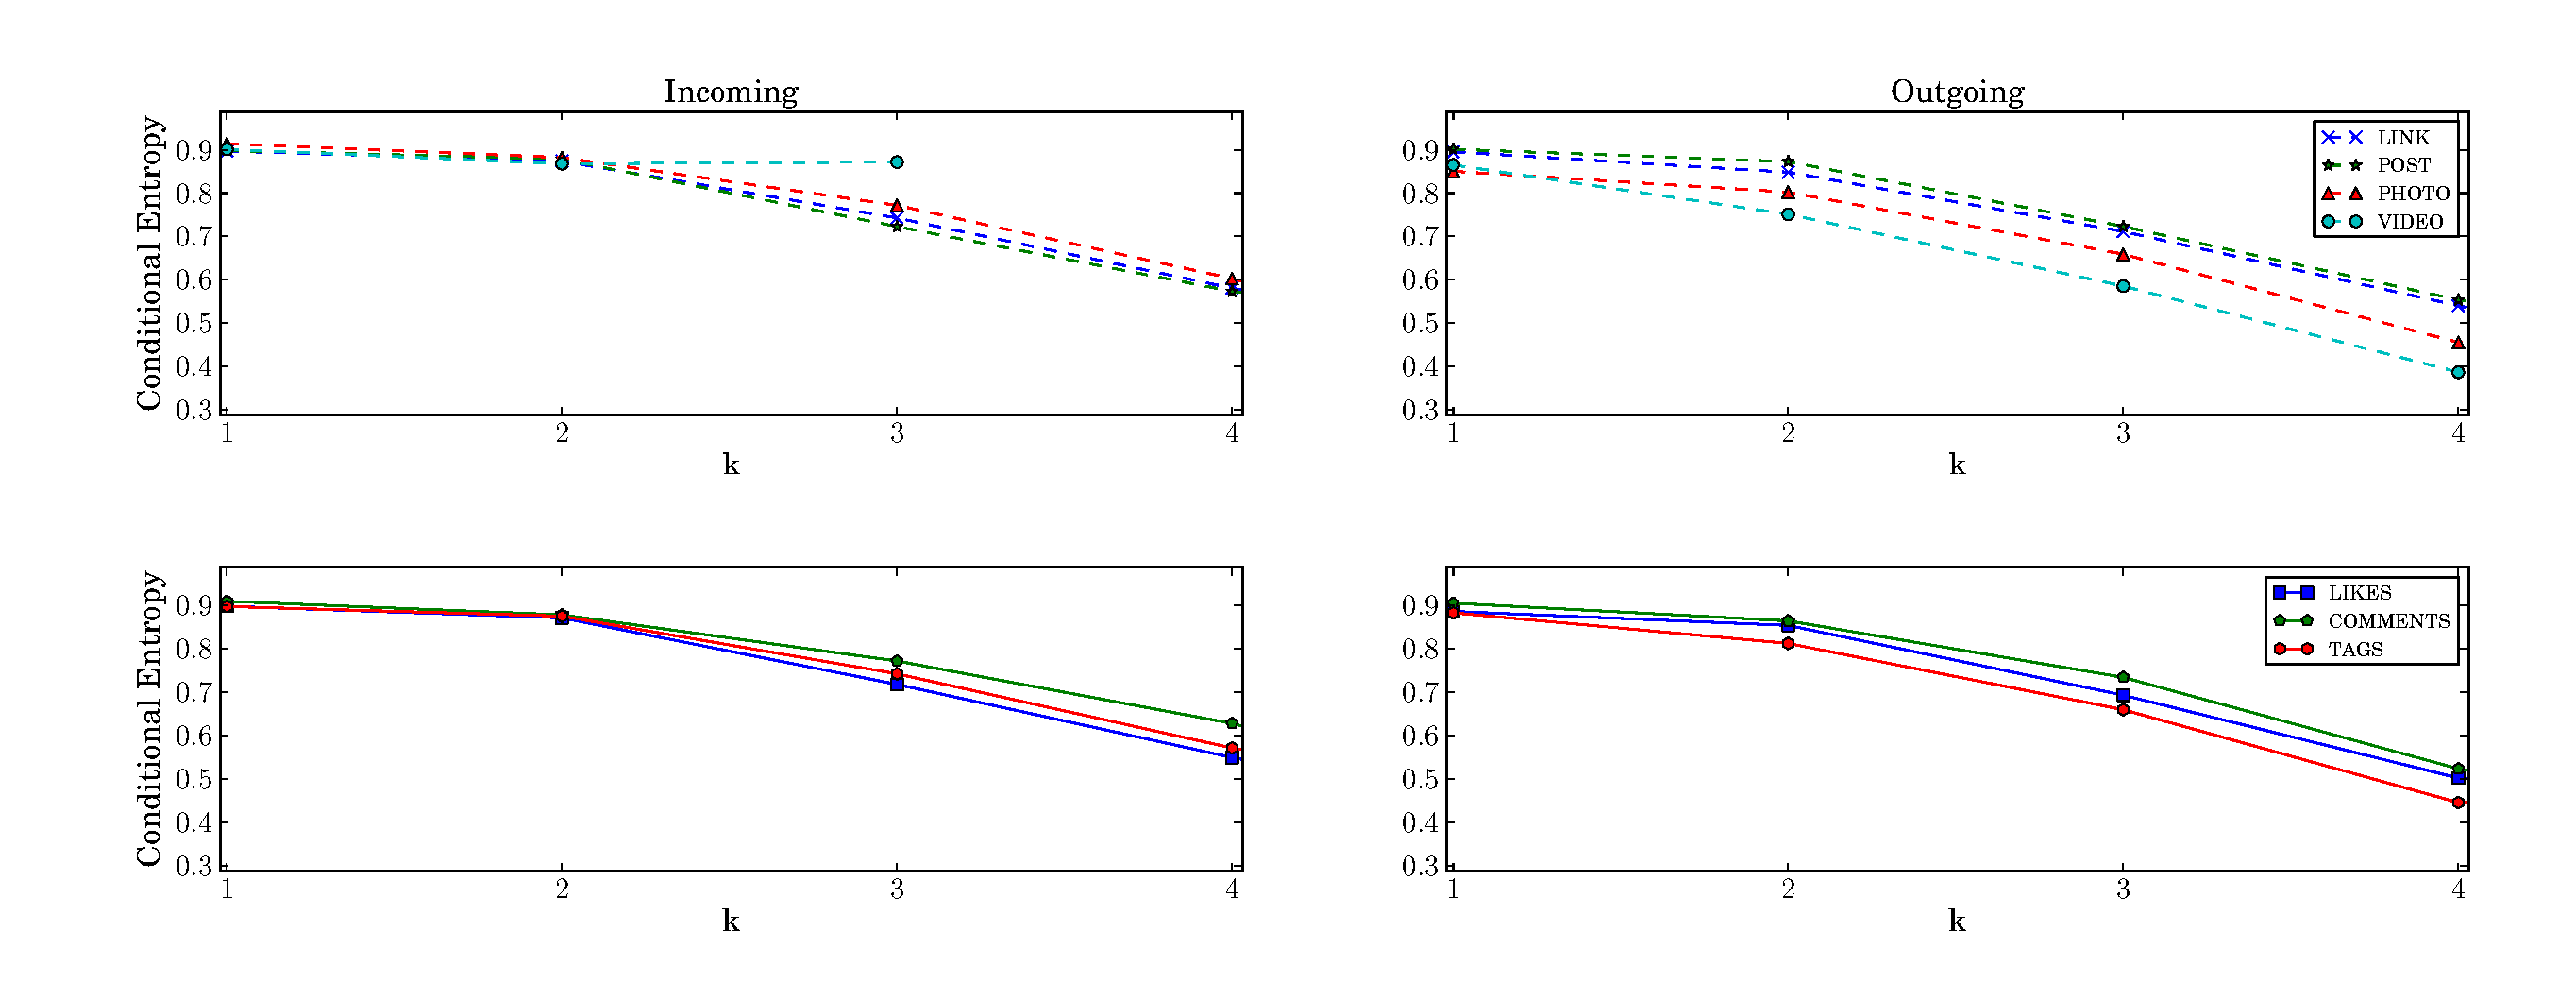
\includegraphics[height=50mm,width=160mm]{data/plots/vsk/ModalityActionsvsKFriends.eps}
%\caption{Conditional Entropy  of modalities/activities for incoming/outgoing interactions vs item liked by at least k friends}
%\label{Fig2} 
%\end{figure*}
%%%%%%%%%%%%%%%%%%%%%%%%%%%%%%%%%%%%%%%%%%%%%%%%%%%%%%%%%%%%%%%%%%%%%%%%%%%
In this section we analyze the informativeness of Interaction SAGs,
namely user interactions according to their modality, type, and direction, 
as described in Section~\ref{sec:methodology}. Similarly, we analyze the 
informativeness of Activity SAGs with respect to its size.

%namely those SAGs that are built w.r.t. a user $u$'s interactions.
A general method for measuring the amount of information that a 
feature $X$ provides w.r.t. predicting another variable $Y$ 
%(in this case likes or dislikes) 
is to calculate its conditional entropy:
\begin{align*}
H(Y&|X=True)\\
& = -\sum_{y\in{(\like,\dislike)}} p(y|X=true) \ln( p(y|X=true))
\end{align*}

In general, a lower conditional entropy indicates a more informative
feature. Here we use entropy conditioned on sparse features $X=True$ 
instead of just $H(Y~|~X)$ or mutual information $I(Y; X)$, as we found 
that the alternatives are highly correlated with (or dominated by) the number of 
occurrences of the feature (or $P(X=True)$), and give trivial results. 

%As defined in Sec~\ref{sec:methodology}, we have three distinctions for user
%interactions: modality, action, and directionality. 
Table~\ref{table:ce_interaction} shows the conditional entropy for Interactions based on modality, action and direction. Here we observe,
\begin{itemize}
\item 
Interaction on {\em videos} seem to have a stronger preferential affinity 
than other modalities such as links, posts and photos.  This could be
  due to the fact that video viewing is time-consuming and users
  inherently only watch the videos of those whose preferences they
  often share.
\item Tagging has a slightly lower conditional entropy than
  commenting and liking, likely because the majority of tags contains 
  person name(s) on Facebook, indicating a direct social interaction. 
  % indicating that tagging.
\item Outgoing interactions are more predictive than incoming interactions.
  It indicates that a user is more likely to share preferences with someone who she
  initiates the interaction with (outgoing) vs. with someone who
  initiates the interaction with her (incoming).  
\end{itemize}

% First we analyze various interactions individually and jointly to understand what
% interactions define SAGs with a high social affinity for a user $u$'s
% preferences.  To this end, we make a few observations from the
% conditional entropy analysis of Table~\ref{table:ce_interaction}:
% \begin{itemize}
% \item Interaction on {\em videos} seem to have a stronger preferential affinity 
% than other modalities such as links, posts and photos.  This could be
%   due to the fact that video viewing is time-consuming and users
%   inherently only watch the videos of those whose preferences they
%   often share.
% \item Tagging has a slightly lower conditional entropy than
%   commenting and liking, likely because the majority of tags contains 
%   person name(s) on Facebook, indicating a direct social interaction. 
%   % indicating that tagging.
% \item A user is more likely to share preferences with someone who she
%   initiates the interaction with (outgoing) vs. with someone who
%   initiates the interaction with her (incoming).  As an extreme
%   instance of this, we note that while outgoing photo and video
%   interactions are most informative, it appears that incoming photo
%   and video interactions are least informative.
% \end{itemize}

% In figure \ref{Fig2} we plot conditional entropy of modality and
% action for incoming/outgoing interactions constrained to links
% liked by at least $k$ friends in the Interaction SAG.  Figure \ref{Fig2} reiterates
% many observations made above for various $k$.  In addition, we note that
% preference affinity with a SAG increases as more people in the SAG
% Note that these graphs are cumulative in $k$, different from the 
% exposure curve on exactly $k$ friends~\cite{Romero2011hashtag}. 
% Our observations on user preference on items like by a number of Facebook friends 
% suggest large cumulative number of friend interactions is more predictive 
% -- this can be translated into recommender system design. 
% Further investigation is needed to pinpoint whether or not there is 
% diminishing returns on repeated exposures~\cite{ver2011stops,Romero2011hashtag} on $k$, 
% and how this could be leveraged to design recommendation algorithms.


%We observed that 
%\begin{itemize}
%% NOTED ABOVE NOW
%  \item Some interactions are more predictive than other. For
%    eg. videos and photo interactions were found to be significantly
%    more predictive than post and link interactions. Similarly,
%    tagging action is often more predictive than commenting and
%    liking.
%  \item As noted by previous work~\cite{saez2011high}, we observe that
%    outgoing interactions are more predictive than incoming
%    interactions. Furthermore, the differentiation between
%    predictiveness modalities and actions is more pronounced in
%    outgoing interactions than in incoming interactions.
%  \item 

%This exhibits repeated exposure properties of epidemic
%models for social networks~\cite{Golub2010selectionbiase}.
%\end{itemize}


%!TEX root = document.tex

% Note: activity SAGs can go beyond friends.

%In this section we evaluate the correlation between the conditional
%entropy and size of groups, pages and favourites.

Fig \ref{Fig3} shows the relationship between conditional
    entropy and the size of activity groups. For public activity ({\em Pages} and 
    {\em Favorites}) size refers to the total number of facebook user in activity group, whereas
    for {\em Groups}(which are generally private) it's total number of user in App 
    user's ego network. Fig \ref{Fig3} shows that the activity groups of small 
    size can be highly predictive whereas large groups are rarely predictive.

In Fig~\ref{Fig4} we plot the average conditional entropy of the top
    10\% of features cumulative up to the size of the activity group given on the
    x-axis; this allows us to determine the marginal contribution of
    larger groups to the average conditional entropy as larger groups
    are incrementally added in.  This graph 
    distinctly shows that the small sized groups, pages and favourites
    have low average conditional entropy that transitions sharply to a
    higher average once a size threshold has been met. From 
    Fig~\ref{Fig4} we can infer that the group sizes up to 50 and
    page/favourite sizes up to $10^{5}$ are most predictive.
    
    
    In Fig~\ref{Fig5}  we analyze the predictiveness of favourites by categories.
    We can see that contents in the ``long-tail'', i.e.,  
    having a large number of occurrences far from the most popular choices, 
    tend to have be the most predictive affinities. Examples of these include
    music, books, movies. On the contrary, generic affinities (e.g. interests) and 
    those with a smaller number of choices (e.g. sports or fav-teams) 
    tend to be less predictive. 

% %{\bf TODO: make this consistent with earlier discussion regarding persistence,
% %temporally sychronized.}

%     We also analyze predictiveness of favourites by categories in
%     Fig~\ref{Fig5}, where the favorite categories are obtained from Facebook API. 

%     %It shows that SAGs consisting of shared interests,
%     %activity, television, and books are on average most predictive, while 
%     %music, movies, favourite teams, sports and athletes are on average
%     %least predictive.  
   
%     We can see that contents in the ``long-tail'', i.e.,  
%     having a large number of occurrences far from the most popular choices, 
%     tend to have be the most predictive affinities. Examples of these include
%     music, books, movies. On the contrary, generic affinities (e.g. interests) and 
%     those with a smaller number of choices (e.g. sports or fav-teams) 
%     tend to be less predictive. 
   
%     %While favourite teams, sports and athletes may be
%     %too focused to offer much predictiveness vs. the other more diverse
%     %categories, it is interesting that movies and music favourites
%     %are not very predictive on average.  This may have to do with the fact that
%     %these are typically ephemeral favourites that may be heavily influenced
%     %by popularity as opposed to true personal preference.
% %\end{itemize}

%In Fig~\ref{Fig4} we plot the average conditional entropy of top
%    10\% features cumulative over the size of activity group. It
%    distinctly shows that the small sized group, pages and favourites
%    have low average conditional entropy. Furthermore, it explains
%    average conditional entropy decreases as size increases. From the
%    figure \ref{Fig4} we can infer that the group size upto 50 and
%    page/favourite size upto $10^{5}$ can be highly predictive.
%
%We also analyze predictiveness of favourites by categories in
%    Fig \ref{Fig5}. It shows that television, books, music and movies
%    are predictive whereas favourite teams, sports and athletes are
%    less predictive.
%\end{itemize}

% %\TODO{add a table of top 5-10 groups/pages/favs}

% \begin{table*}[tbp!]
% \centering
% \begin{tabular}{| >{\small}l | >{\small}r | >{\small}r |}
% \hline
% \textbf{Top Groups} & \textbf{Top Pages} & \textbf{Top Favourites} \\
% \hline
% %Heavy Metal - Australian Capital Territory & Avascular Necrosis & Avascular Necrosis \\
% Heavy Metal - (city name) & Avascular Necrosis & Avascular Necrosis \\
% Stephen Conroy Should Not Filter Our Internet & Assidian & Tortured \\
% Silicone Stripper & Tortured & Elysian \\
% Hardcore dancing is not moshing & Elysian & Anno Domini \\
% %Metal bands come to Canberra cause I'm sick of... & Darker Half & Hellbringer \\
% Metal bands come to (city name) cause I'm sick of... & Darker Half & Hellbringer \\
% %Canberra Rock Gigs & Johnny Roadkill & Johnny Roadkill \\
% (city name) Rock Gigs & Johnny Roadkill & Johnny Roadkill \\
% %Let's Mosh - Canberra metal radio show - 2XX 9 & Anno Domini & Darker Half \\
% Let's Mosh - (city name) metal radio show - 2XX 9 & Anno Domini & Darker Half \\
% Bring Steel Panther to Australia & Billy Madison & Bane Of Isildur \\
% %Canberra Death/Heavy Metal Appreciation & Hellbringer & Katabasis \\
% (city name)  Death/Heavy Metal Appreciation & Hellbringer & Katabasis \\
% Robert The Bruce (Band) & Metalocalypse & Aeon of Horus \\
% \hline
% \end{tabular}
% \caption{Top 10 Groups/Pages/Favourites ranked by Conditional Entropy. The city name where our institution and many Facebook users resides is anonymized.}
% \label {table:topGroupPagesFavs}
% \end{table*}



%%%%%%%%%%%%%%%%%%%%%%%%%%%%%%%%%%%%%%%%%%%%%%%%%%%%%%%%%%%%%%%%%%%%%%%%%%%
\begin{figure}[tbp!]
%\centering
\hspace{-8mm}
\begin{tabular}{ccc}
\subfloat[Fig:][]{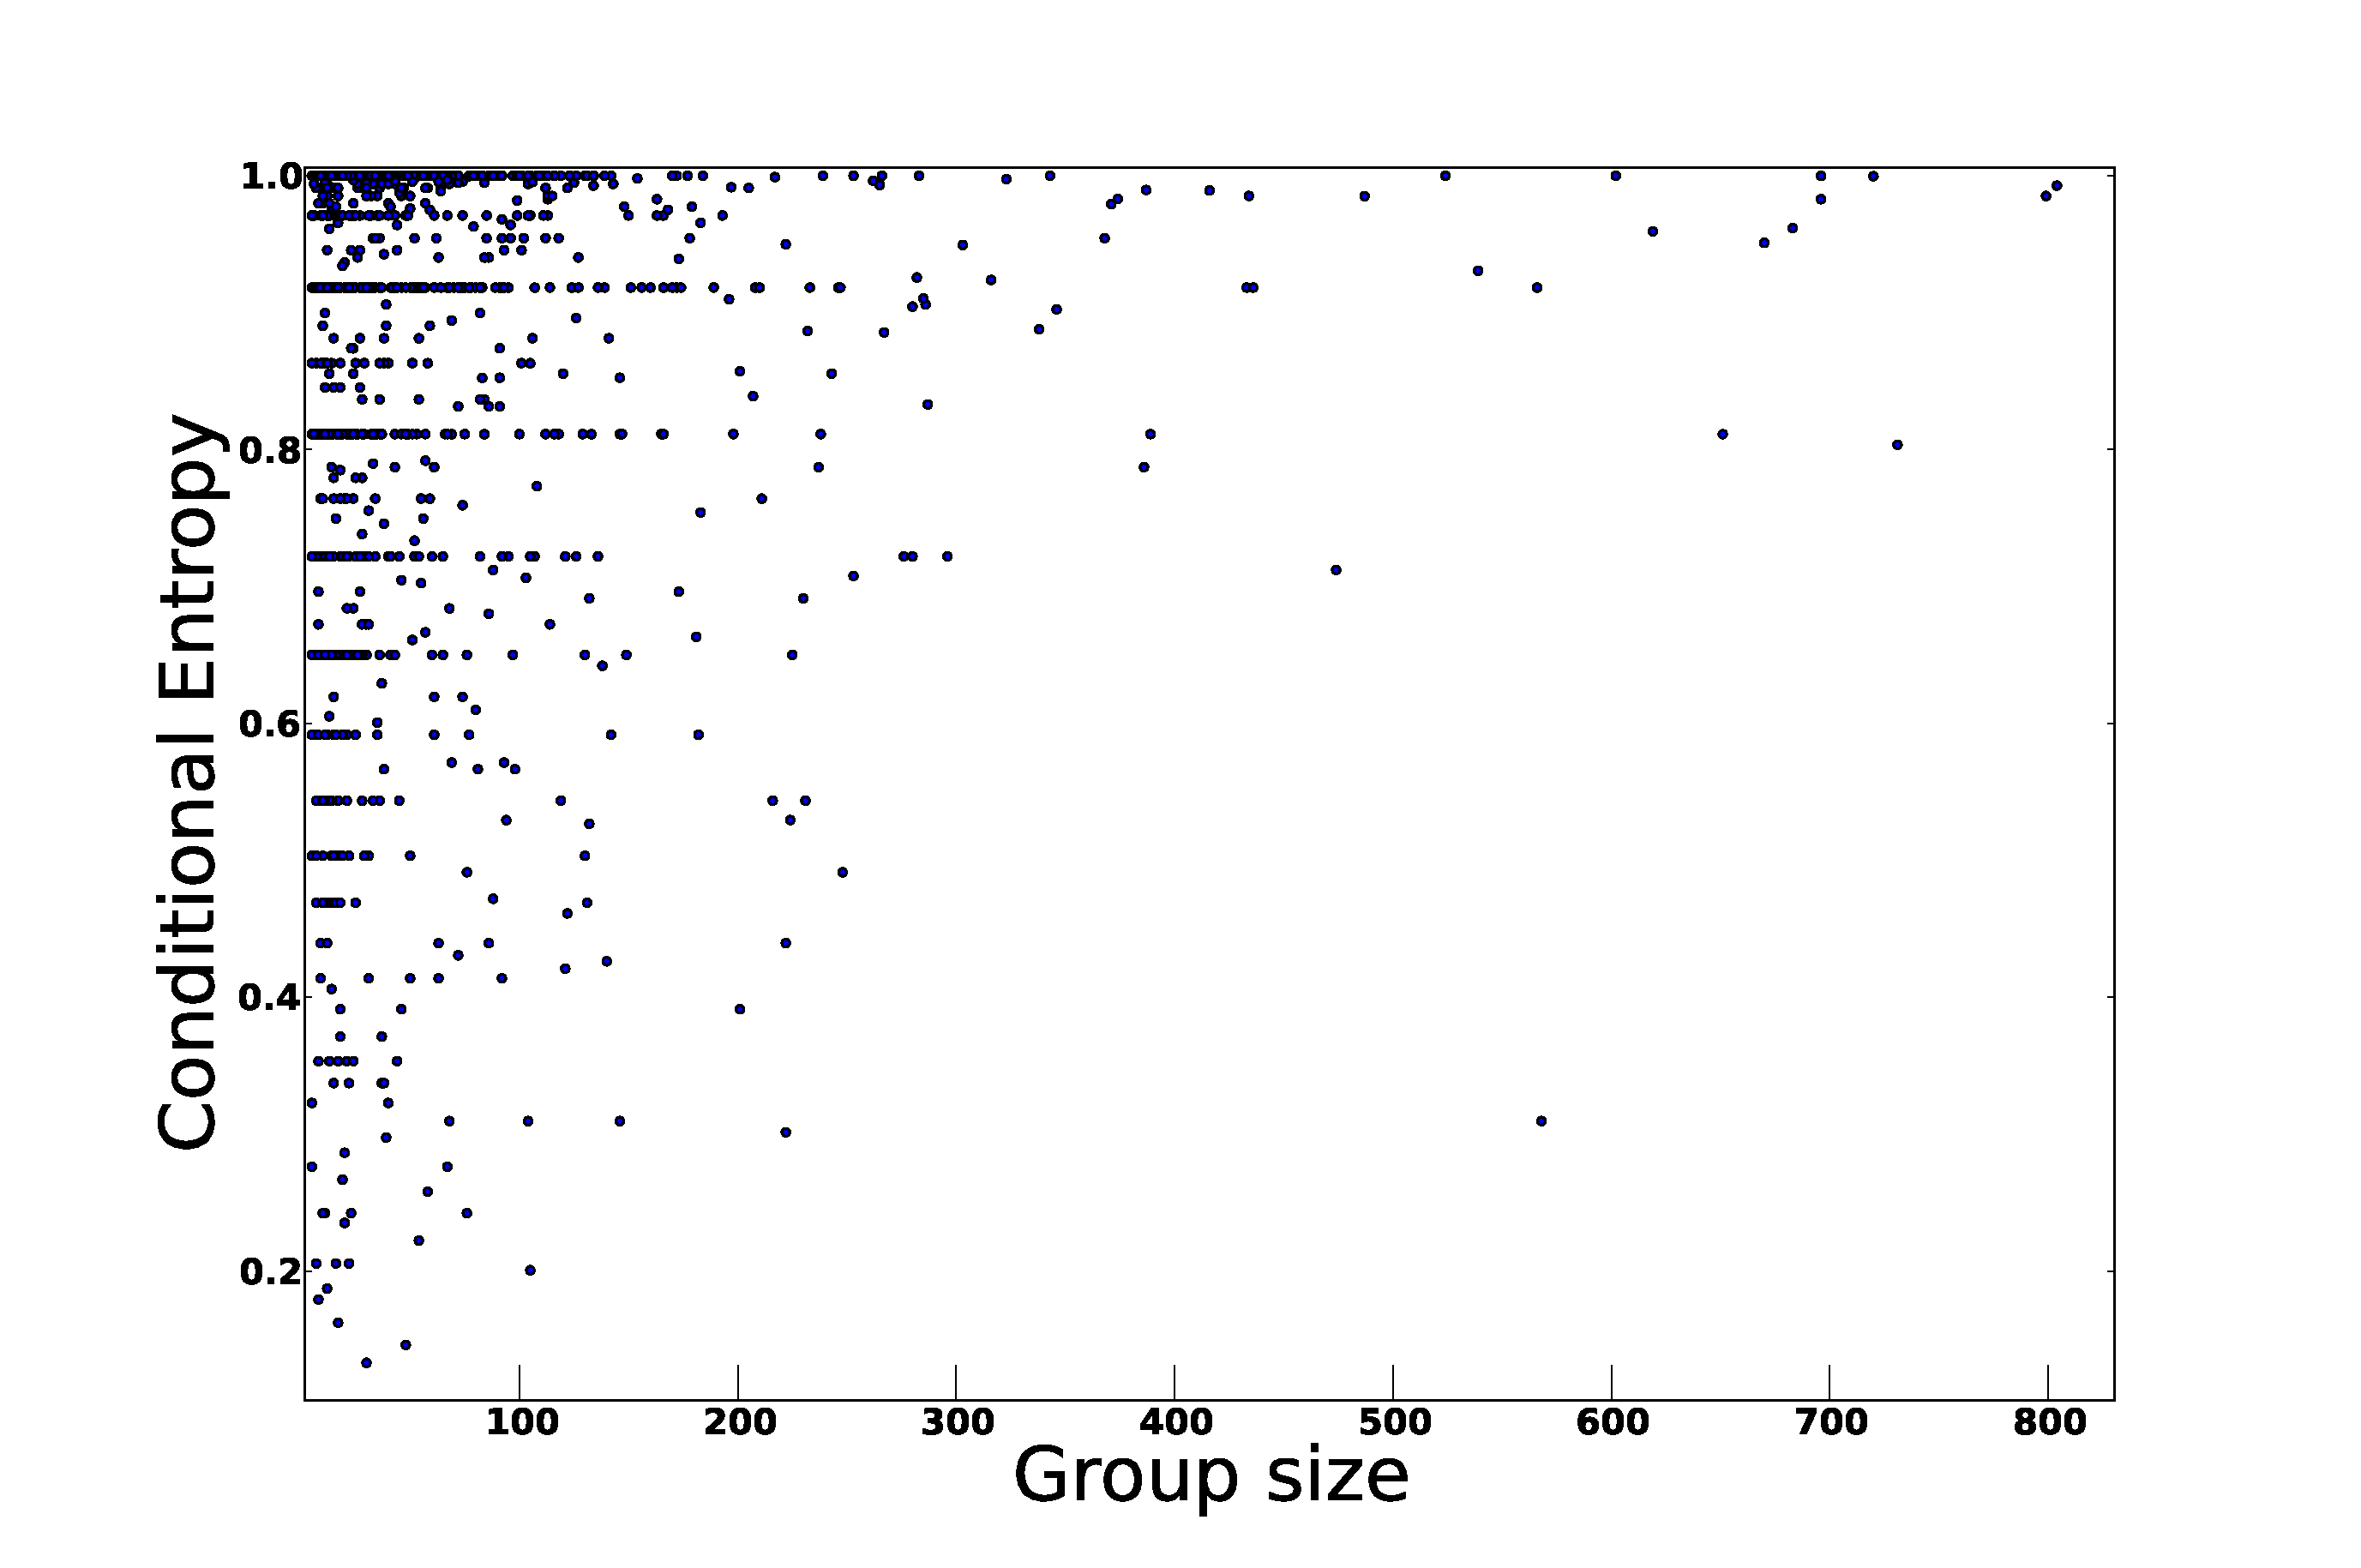
\includegraphics[width=32mm, height=30mm]{data/plots/new/CEvsGroupSize.eps}}
\subfloat[Fig:][]{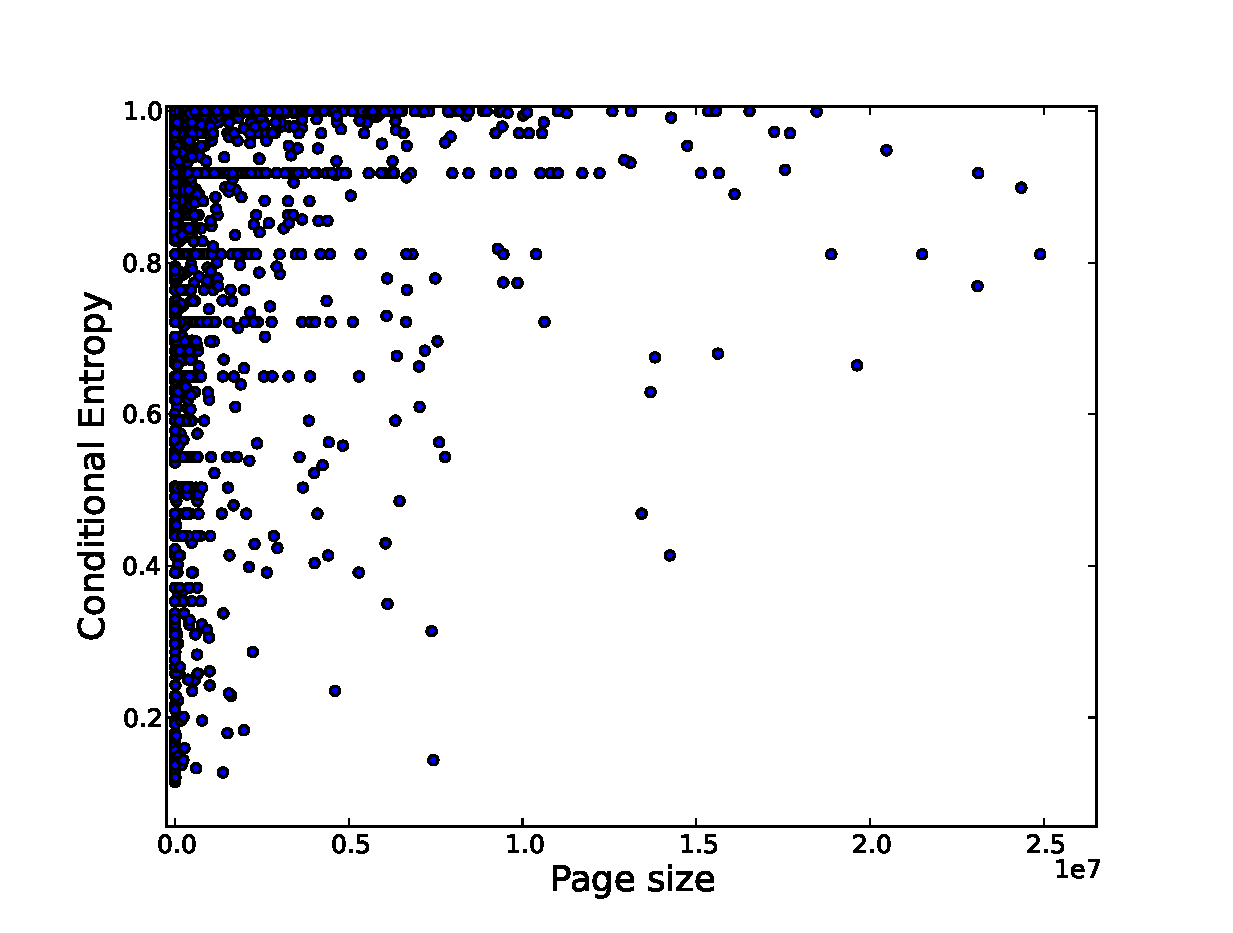
\includegraphics[width=32mm, height=30mm]{data/plots/new/CEvsPageSize.eps}}
\subfloat[Fig:][]{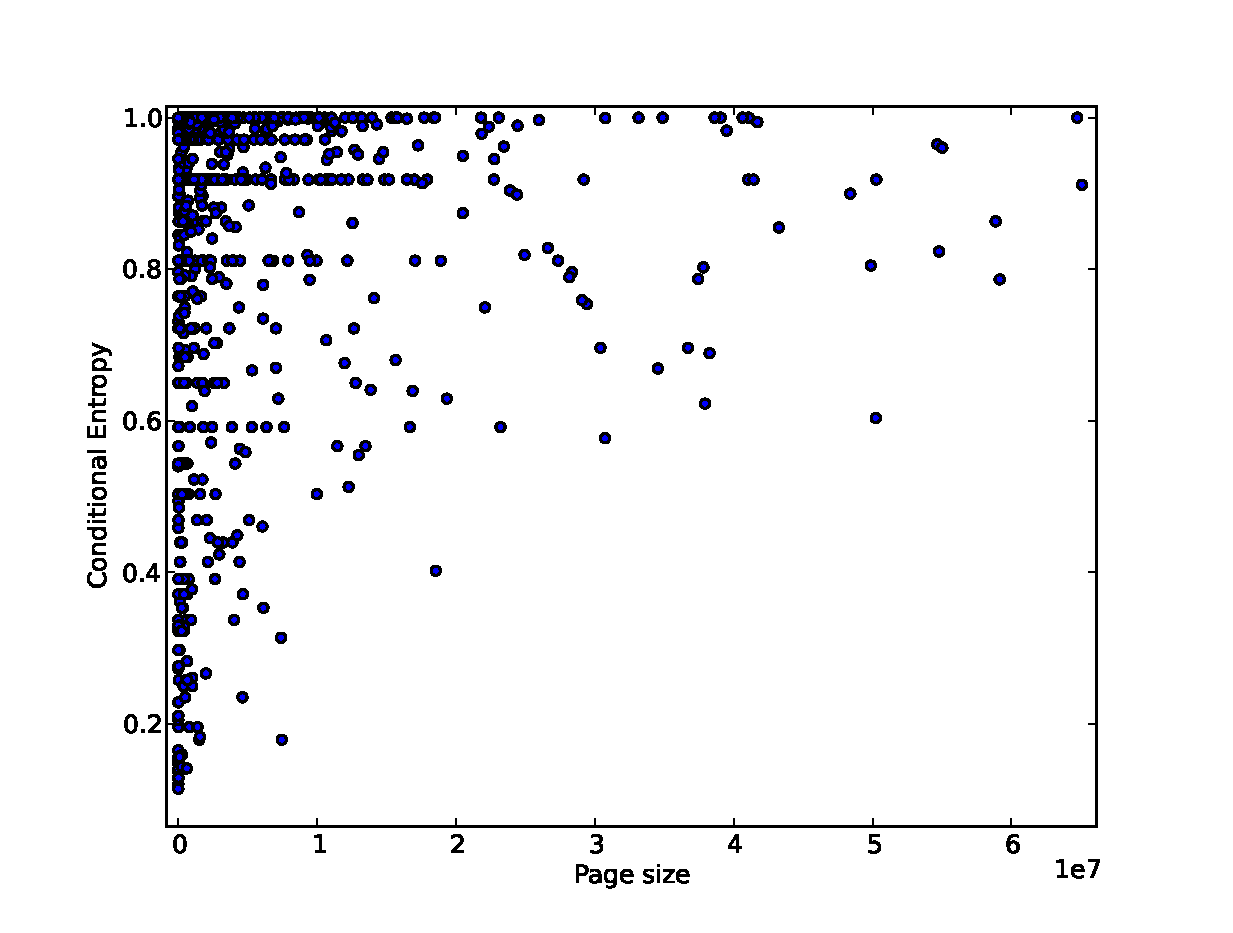
\includegraphics[width=32mm, height=30mm]{data/plots/new/CEvsFavSize.eps}}
\end{tabular}
\caption {Conditional entropy vs size }
\label{Fig3}
\end{figure}
%%%%%%%%%%%%%%%%%%%%%%%%%%%%%%%%%%%%%%%%%%%%%%%%%%%%%%%%%%%%%%%%%%%%%%%%%%%

% %%%%%%%%%%%%%%%%%%%%%%%%%%%%%%%%%%%%%%%%%%%%%%%%%%%%%%%%%%%%%%%%%%%%%%%%%%%
% \begin{figure}[tbp!]
% %\centering
% \hspace{-10mm}
% \begin{tabular}{ccc}
% \begin{tabular}{ccc}
% \subfloat[Fig:][]{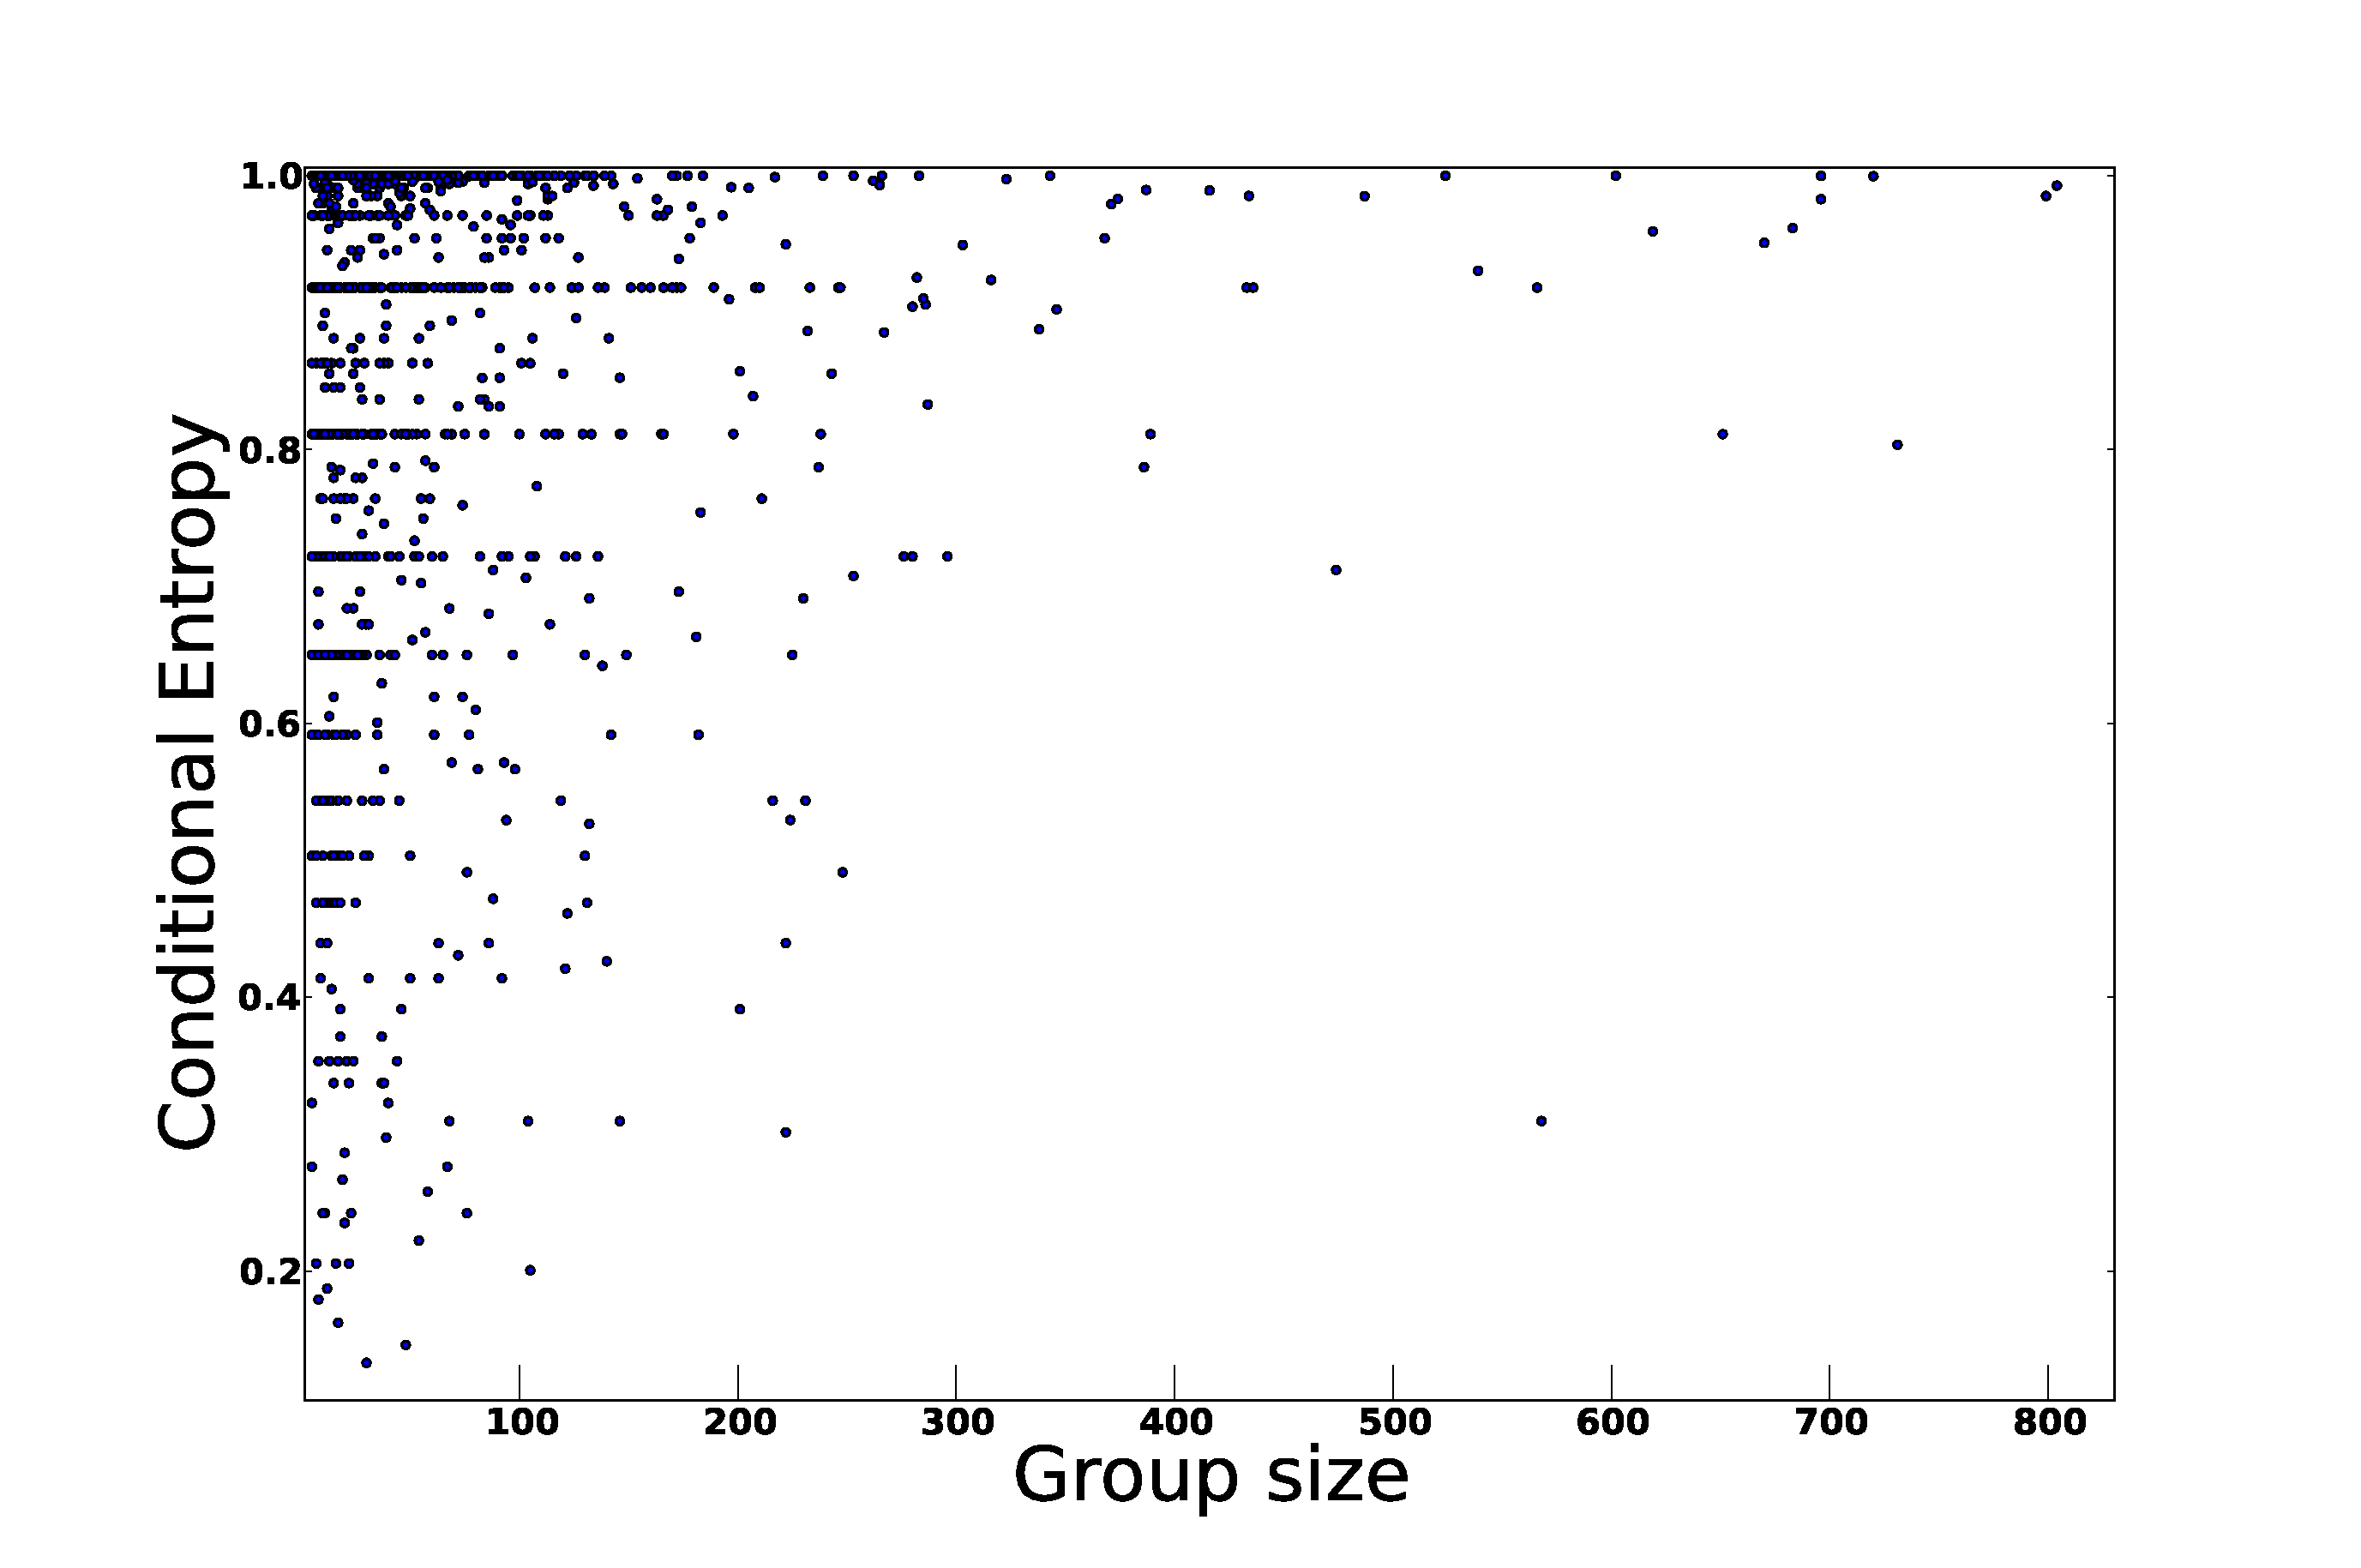
\includegraphics[width=32mm, height=30mm]{data/plots/new/CEvsGroupSize.eps}}
% \subfloat[Fig:][]{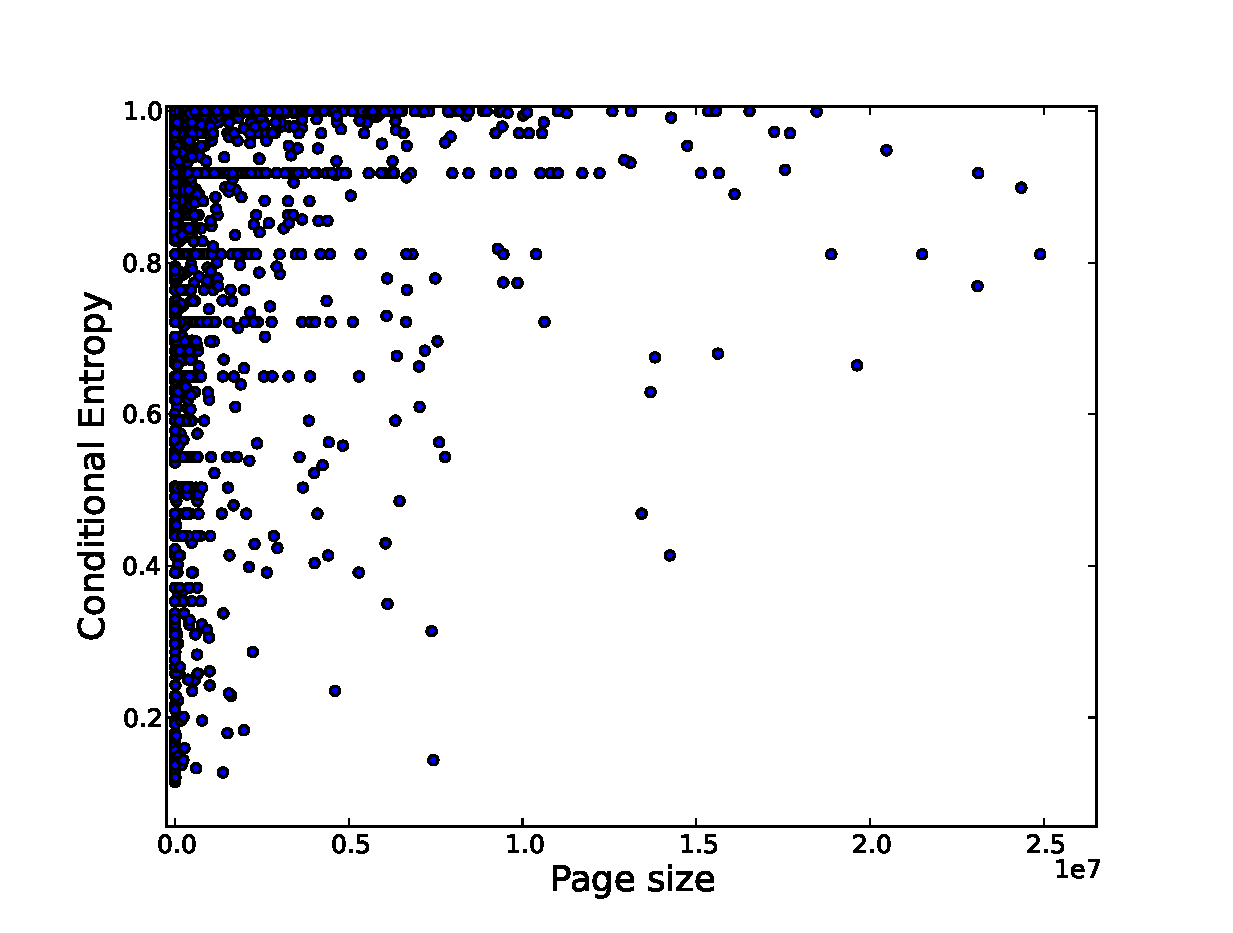
\includegraphics[width=32mm, height=30mm]{data/plots/new/CEvsPageSize.eps}}
% \subfloat[Fig:][]{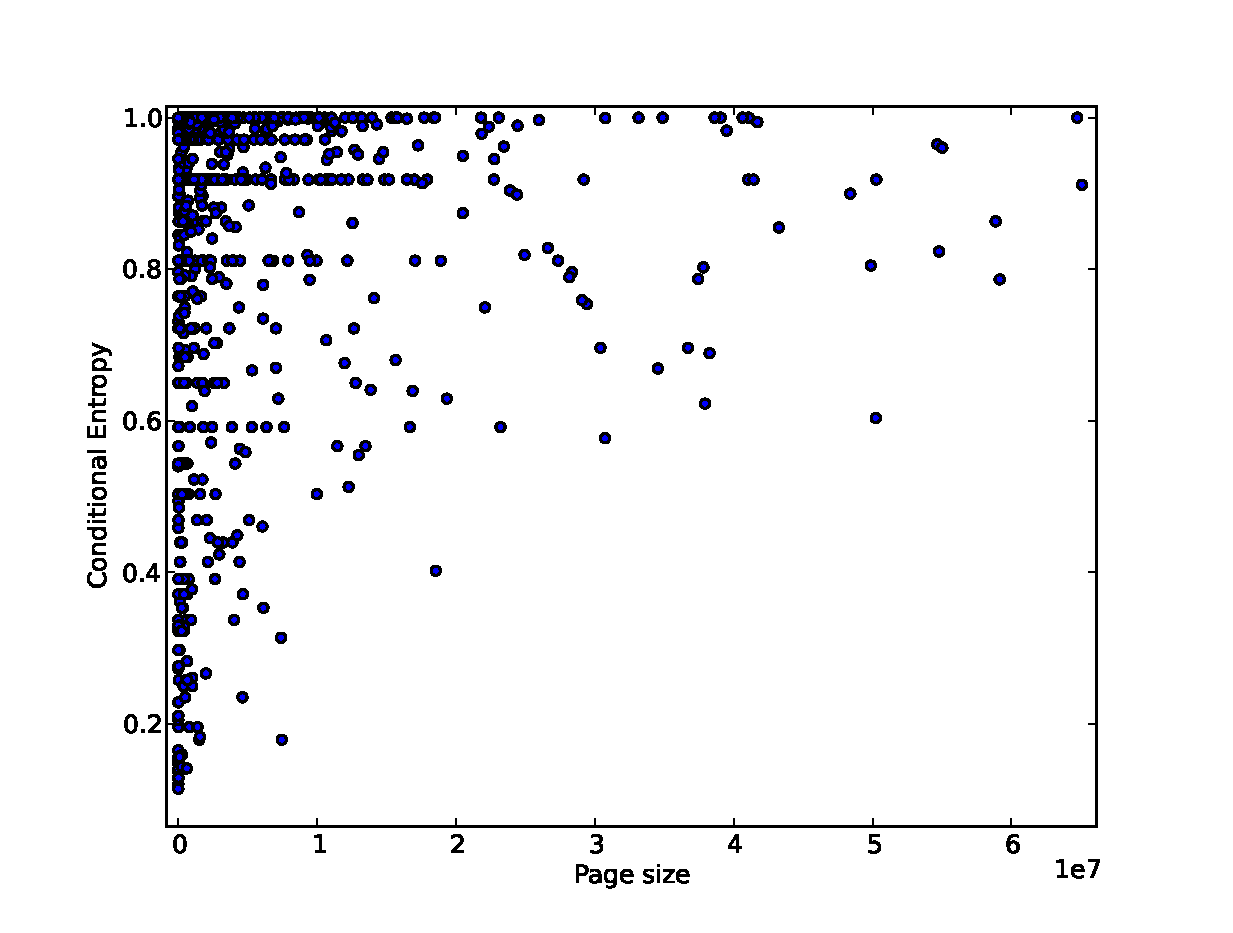
\includegraphics[width=32mm, height=30mm]{data/plots/new/CEvsFavSize.eps}} \\
% \subfloat[Fig:][]{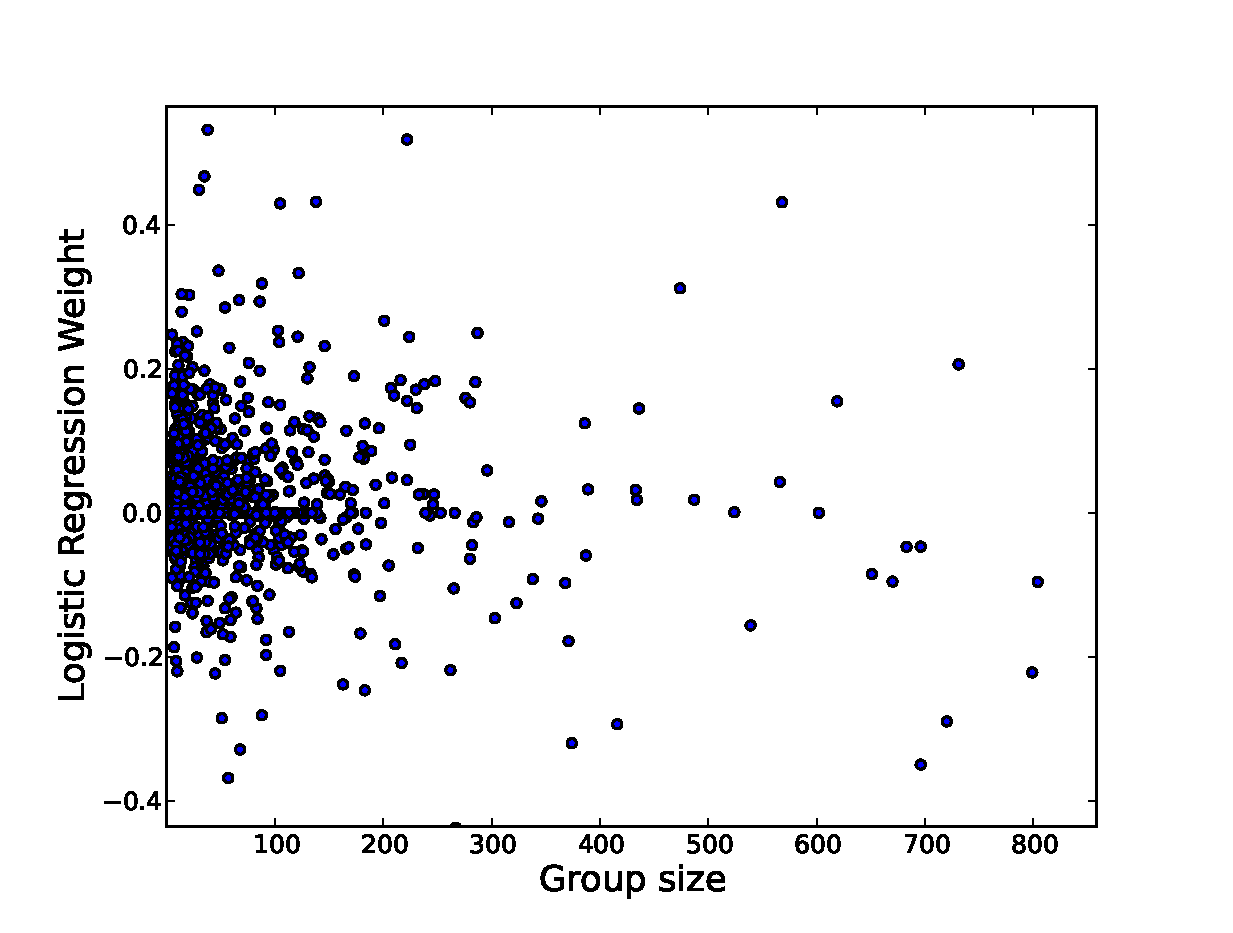
\includegraphics[width=32mm, height=30mm]{data/plots/new/LRweightvsGroupSize.eps}}
% \subfloat[Fig:][]{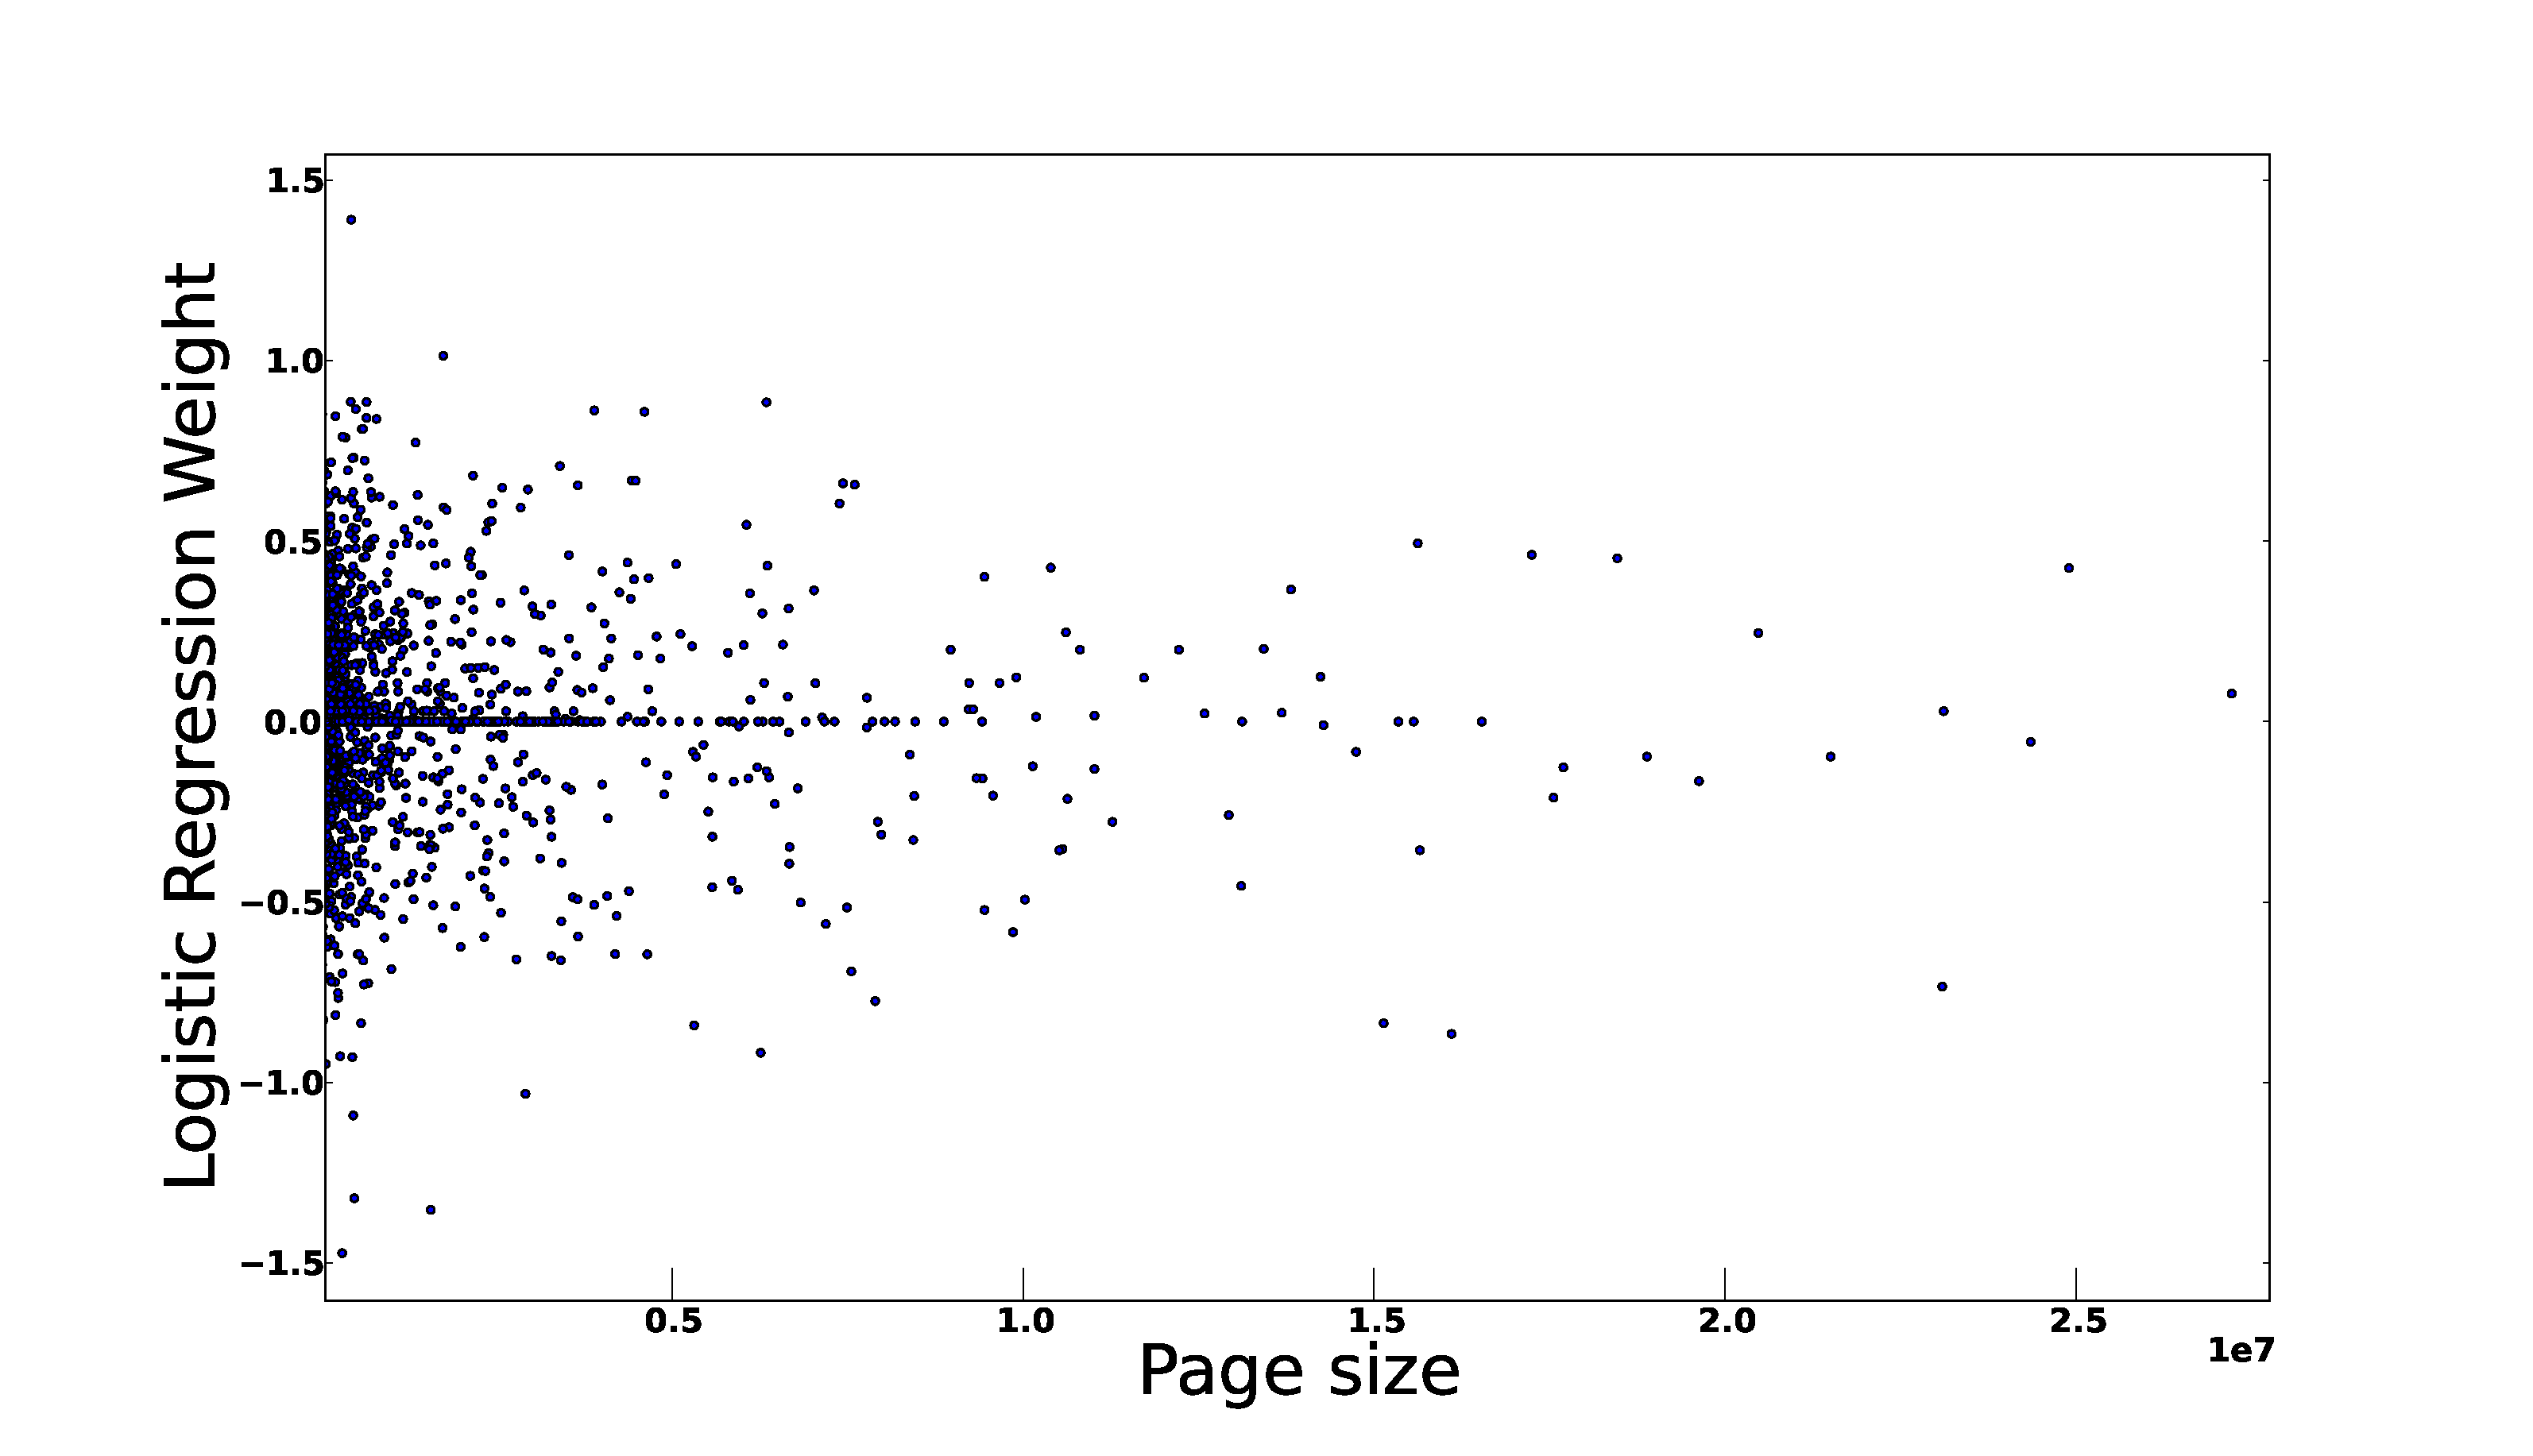
\includegraphics[width=32mm, height=30mm]{data/plots/new/LRweightvsPageSize.eps}}
% \subfloat[Fig:][]{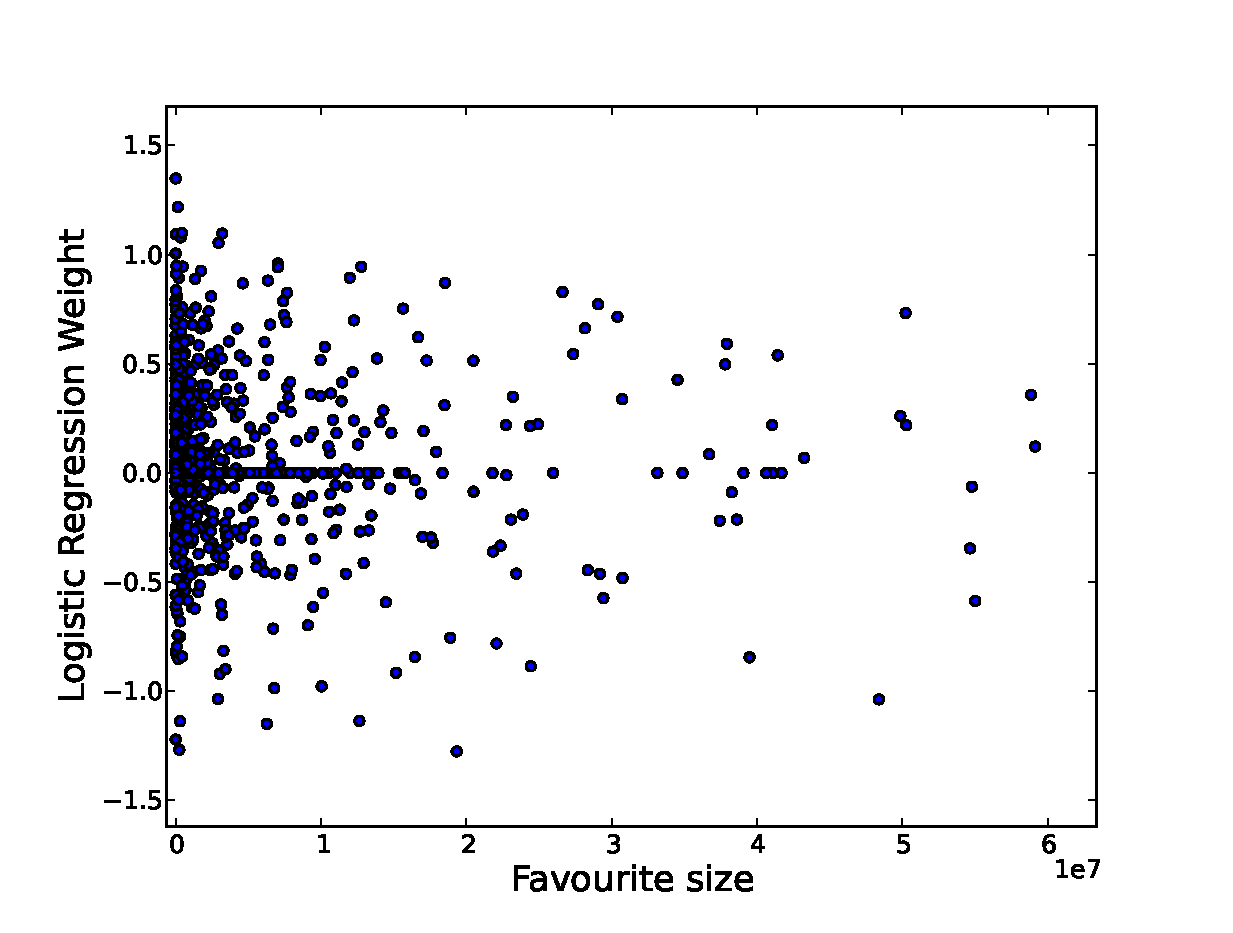
\includegraphics[width=32mm, height=30mm]{data/plots/new/LRweightvsFavSize.eps}} \\
% \end{tabular}
% \end{tabular}
% \caption {Conditional entropy vs size (a-c); logistic regression feature weights vs size (d-f) }
% \label{Fig3}
% \end{figure}
% %%%%%%%%%%%%%%%%%%%%%%%%%%%%%%%%%%%%%%%%%%%%%%%%%%%%%%%%%%%%%%%%%%%%%%%%%%%

%%%%%%%%%%%%%%%%%%%%%%%%%%%%%%%%%%%%%%%%%%%%%%%%%%%%%%%%%%%%%%%%%%%%%%%%%%%
\begin{figure*}[tbp!]
\centering
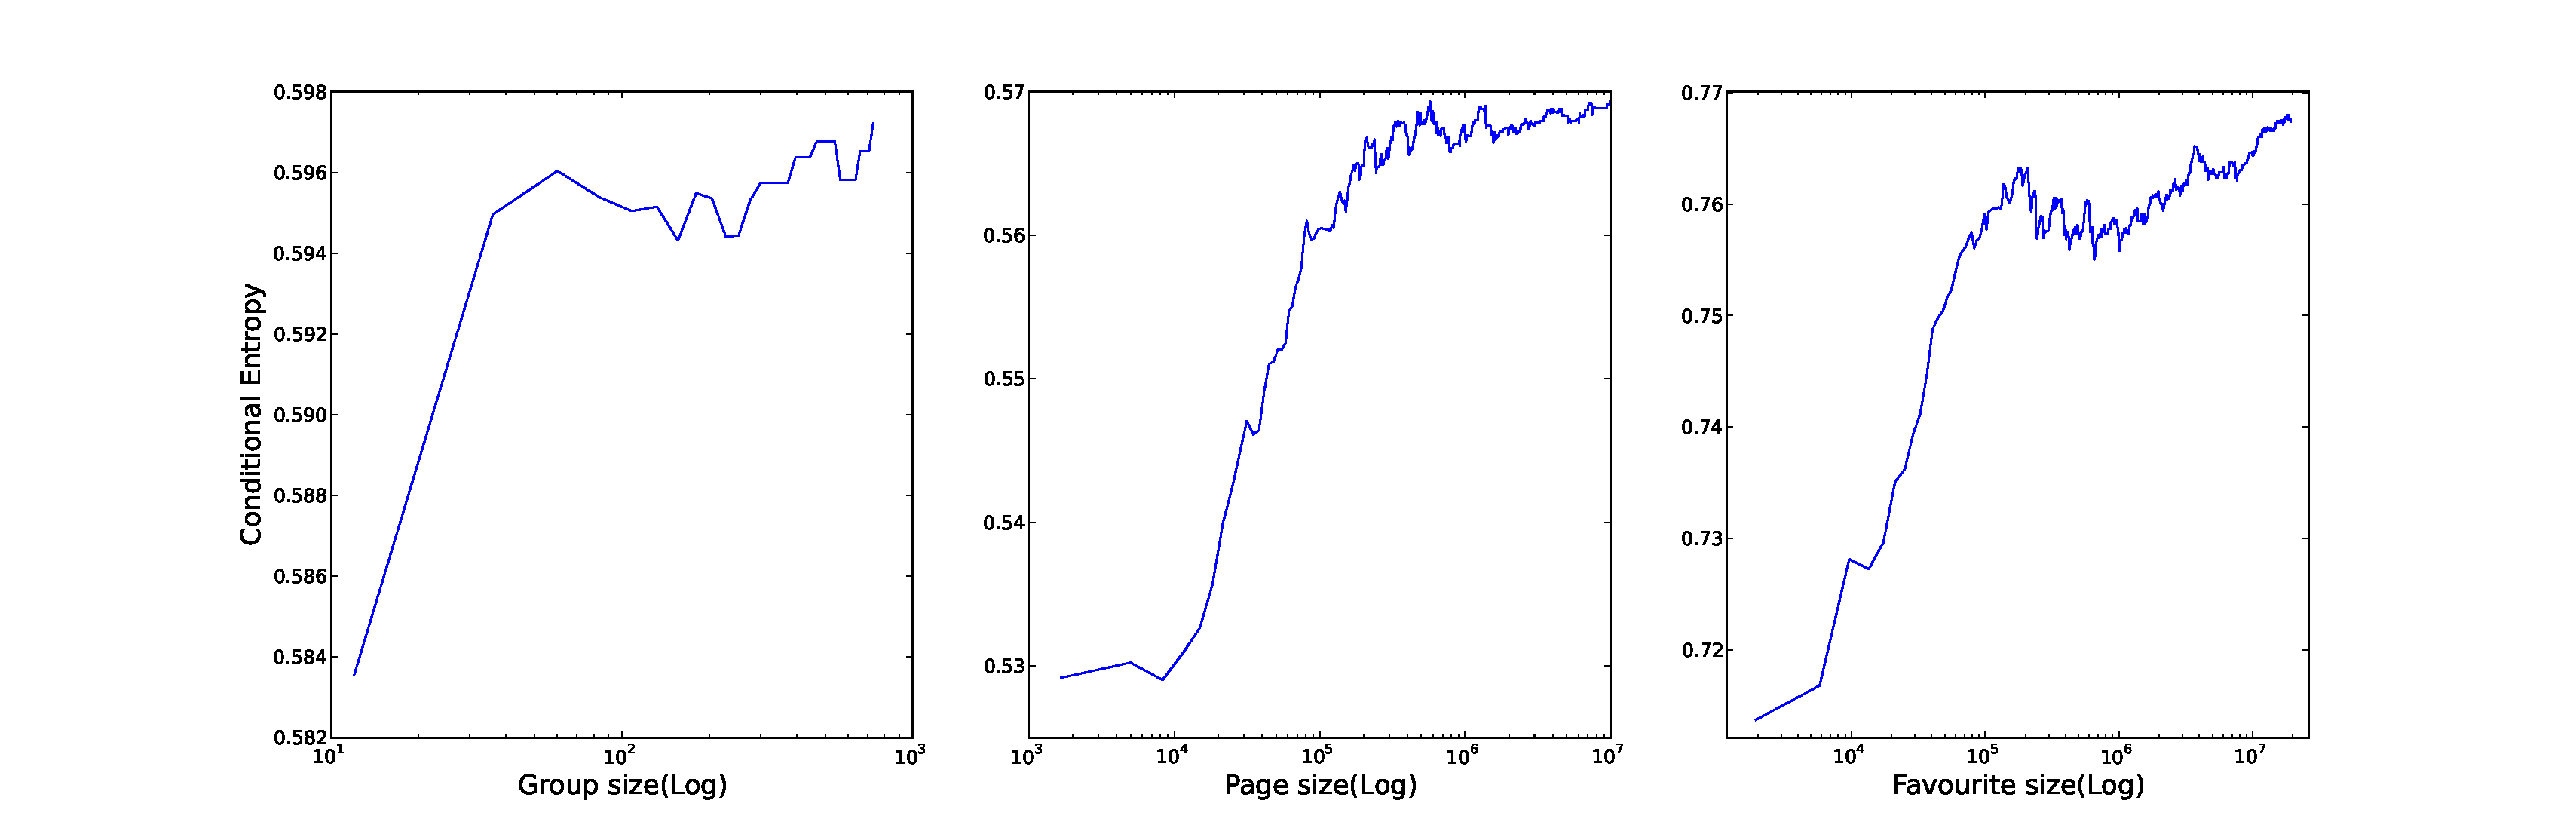
\includegraphics[width=160mm,height=35mm]{data/plots/cumulativeEntropy/cumulative.eps}
\caption{Average conditional entropy of top 10\% groups, pages and favourites features cumulative over the size }
\label{Fig4}
\end{figure*}
%%%%%%%%%%%%%%%%%%%%%%%%%%%%%%%%%%%%%%%%%%%%%%%%%%%%%%%%%%%%%%%%%%%%%%%%%%%

%%%%%%%%%%%%%%%%%%%%%%%%%%%%%%%%%%%%%%%%%%%%%%%%%%%%%%%%%%%%%%%%%%%%%%%%%%%
\begin{figure*}[tbp!]
\centering
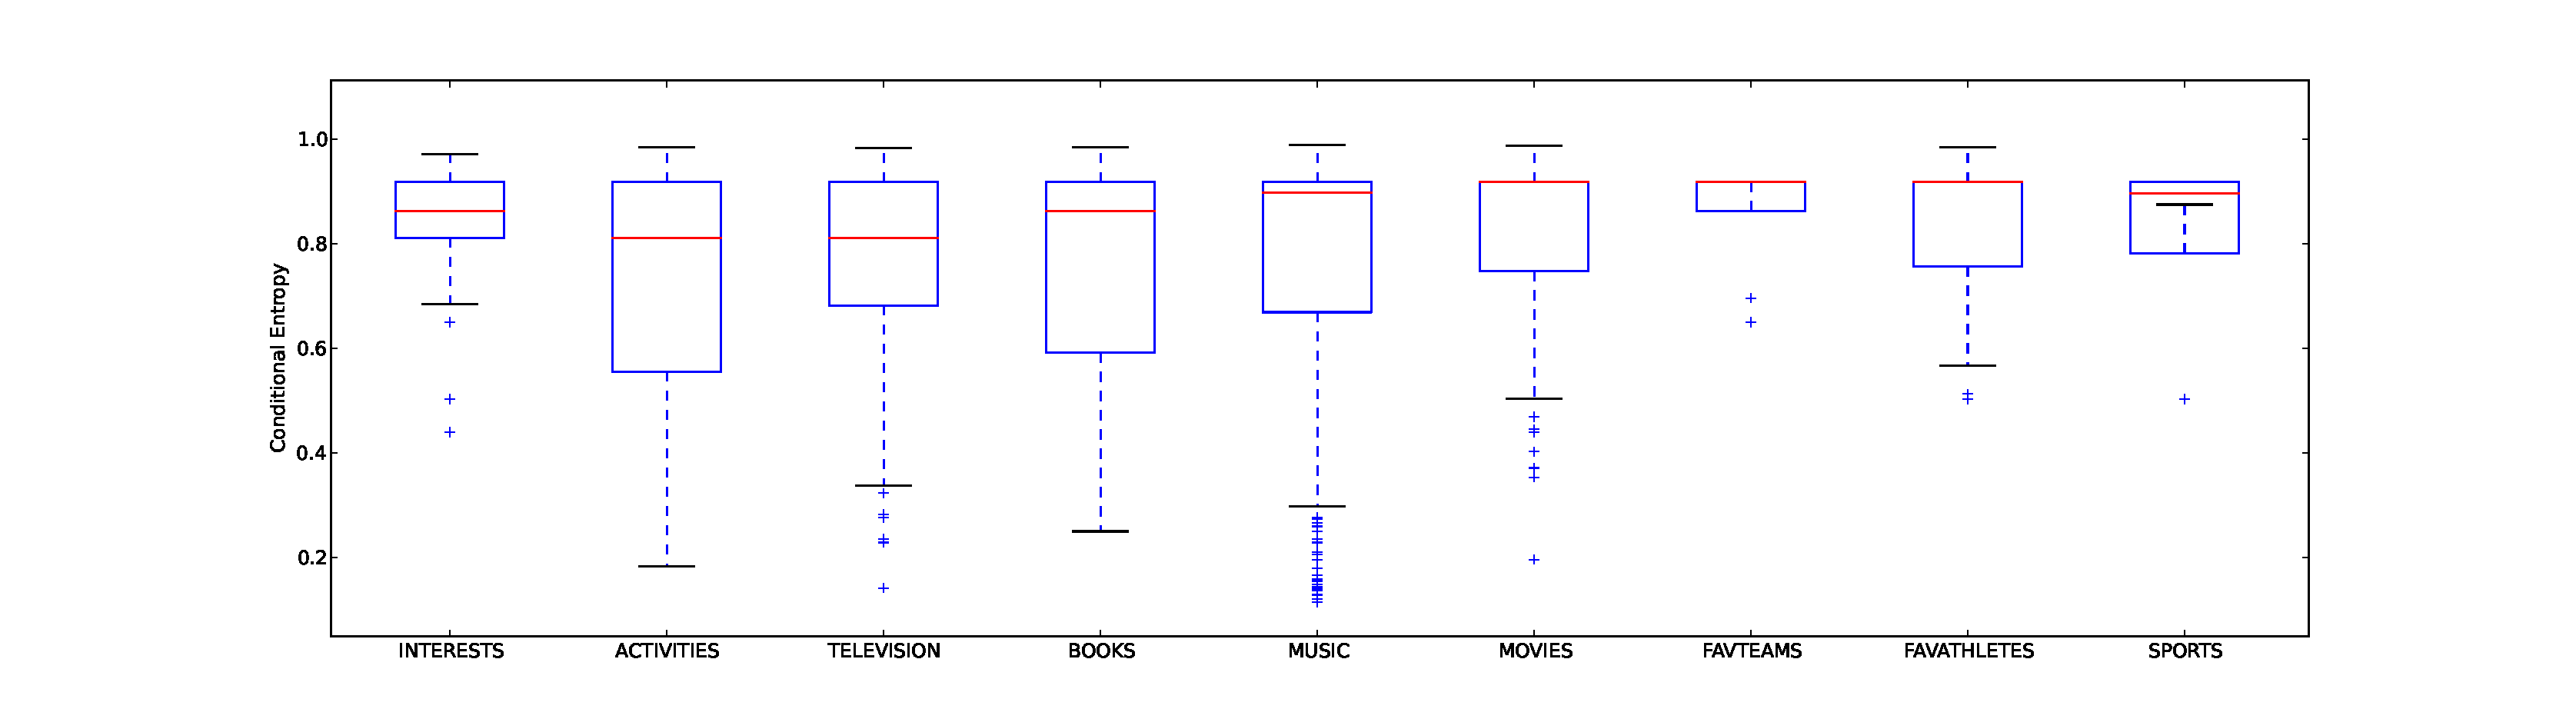
\includegraphics[width=160mm, height=35mm]{data/plots/boxPlots/CEvsFavTypes.eps}
\caption{Conditional entropy for top 1000 favourites breakdown by categories}
\label{Fig5}
\end{figure*}
%%%%%%%%%%%%%%%%%%%%%%%%%%%%%%%%%%%%%%%%%%%%%%%%%%%%%%%%%%%%%%%%%%%%%%%%%%%


%\subsection{Interaction Analysis}
%\label{sec:interaction_analysis}

%%!TEX root = document.tex

%%%%%%%%%%%%%%%%%%%%%%%%%%%%%%%%%%%%%%%%%%%%%%%%%%%%%%%%%%%%%%%%%%%%%%%%%%%
\begin{table}
\caption{Conditional entropy of various interactions (lower conditional
entropies are more informative).}
\label{table:ce_interaction}
\vspace{-2mm}
\centering
{\footnotesize
	\begin{tabular}{| >{\small}l | >{\small}r | }
		\hline
		\textbf{ Modality ($X$)} & $H(Y|X=true)$ \\
		\hline
		{ video } & 0.850 \\
		\hline
		{ link } & 0.915 \\
		\hline
		{ post } & 0.918 \\
		\hline
		{ photo } & 0.926 \\
		\hline
\multicolumn{2}{c}{}\\
		\hline
		\textbf{Action Type ($X$)}  & $H(Y|X=true)$ \\
		\hline
		{ tags }  &  0.920 \\
		\hline
		{ comments }  &  0.921 \\
		\hline
		{ likes }  &  0.924 \\
		\hline
\multicolumn{2}{c}{}\\
		\hline
		\textbf{ Direction ($X$) } & $H(Y|X=true)$ \\
		\hline
		{ outgoing }  &  0.928 \\
		\hline
		{ incoming }  &  0.935 \\
		\hline
\multicolumn{2}{c}{}\\
%	\end{tabular}
%\end{table*}
%%%%%%%%%%%%%%%%%%%%%%%%%%%%%%%%%%%%%%%%%%%%%%%%%%%%%%%%%%%%%%%%%%%%%%%%%%%
%	
%%%%%%%%%%%%%%%%%%%%%%%%%%%%%%%%%%%%%%%%%%%%%%%%%%%%%%%%%%%%%%%%%%%%%%%%%%%
%\begin{table*}
%	\begin{tabular}{| >{\small}l | >{\small}r |}
		\hline
		\textbf{Modality-Direction} ($X$) & $H(Y|X=true)$ \\
		\hline
		tags-outgoing & 0.885 \\
		likes-outgoing & 0.885 \\
		tags-incoming & 0.900 \\
		likes-incoming & 0.902 \\
		comments-outgoing & 0.908 \\
		comments-incoming & 0.912 \\
		\hline
%	\end{tabular}
\multicolumn{2}{c}{}\\
%	\begin{tabular}{| >{\small}l | >{\small}r |}
                \hline	
		\textbf{Action-Direction} ($X$) & $H(Y|X=true)$ \\
		\hline
		photo-outgoing & 0.857 \\
		video-outgoing & 0.863 \\
		link-outgoing & 0.895 \\
		link-incoming & 0.896 \\
		post-incoming & 0.902 \\
		post-outgoing & 0.906 \\
		video-incoming & 0.915 \\
		photo-incoming & 0.921 \\
		\hline
				
	\end{tabular}}
\end{table}
%%%%%%%%%%%%%%%%%%%%%%%%%%%%%%%%%%%%%%%%%%%%%%%%%%%%%%%%%%%%%%%%%%%%%%%%%%%

%%%%%%%%%%%%%%%%%%%%%%%%%%%%%%%%%%%%%%%%%%%%%%%%%%%%%%%%%%%%%%%%%%%%%%%%%%%
\begin{figure*}[tbp!]
\hspace{-15mm}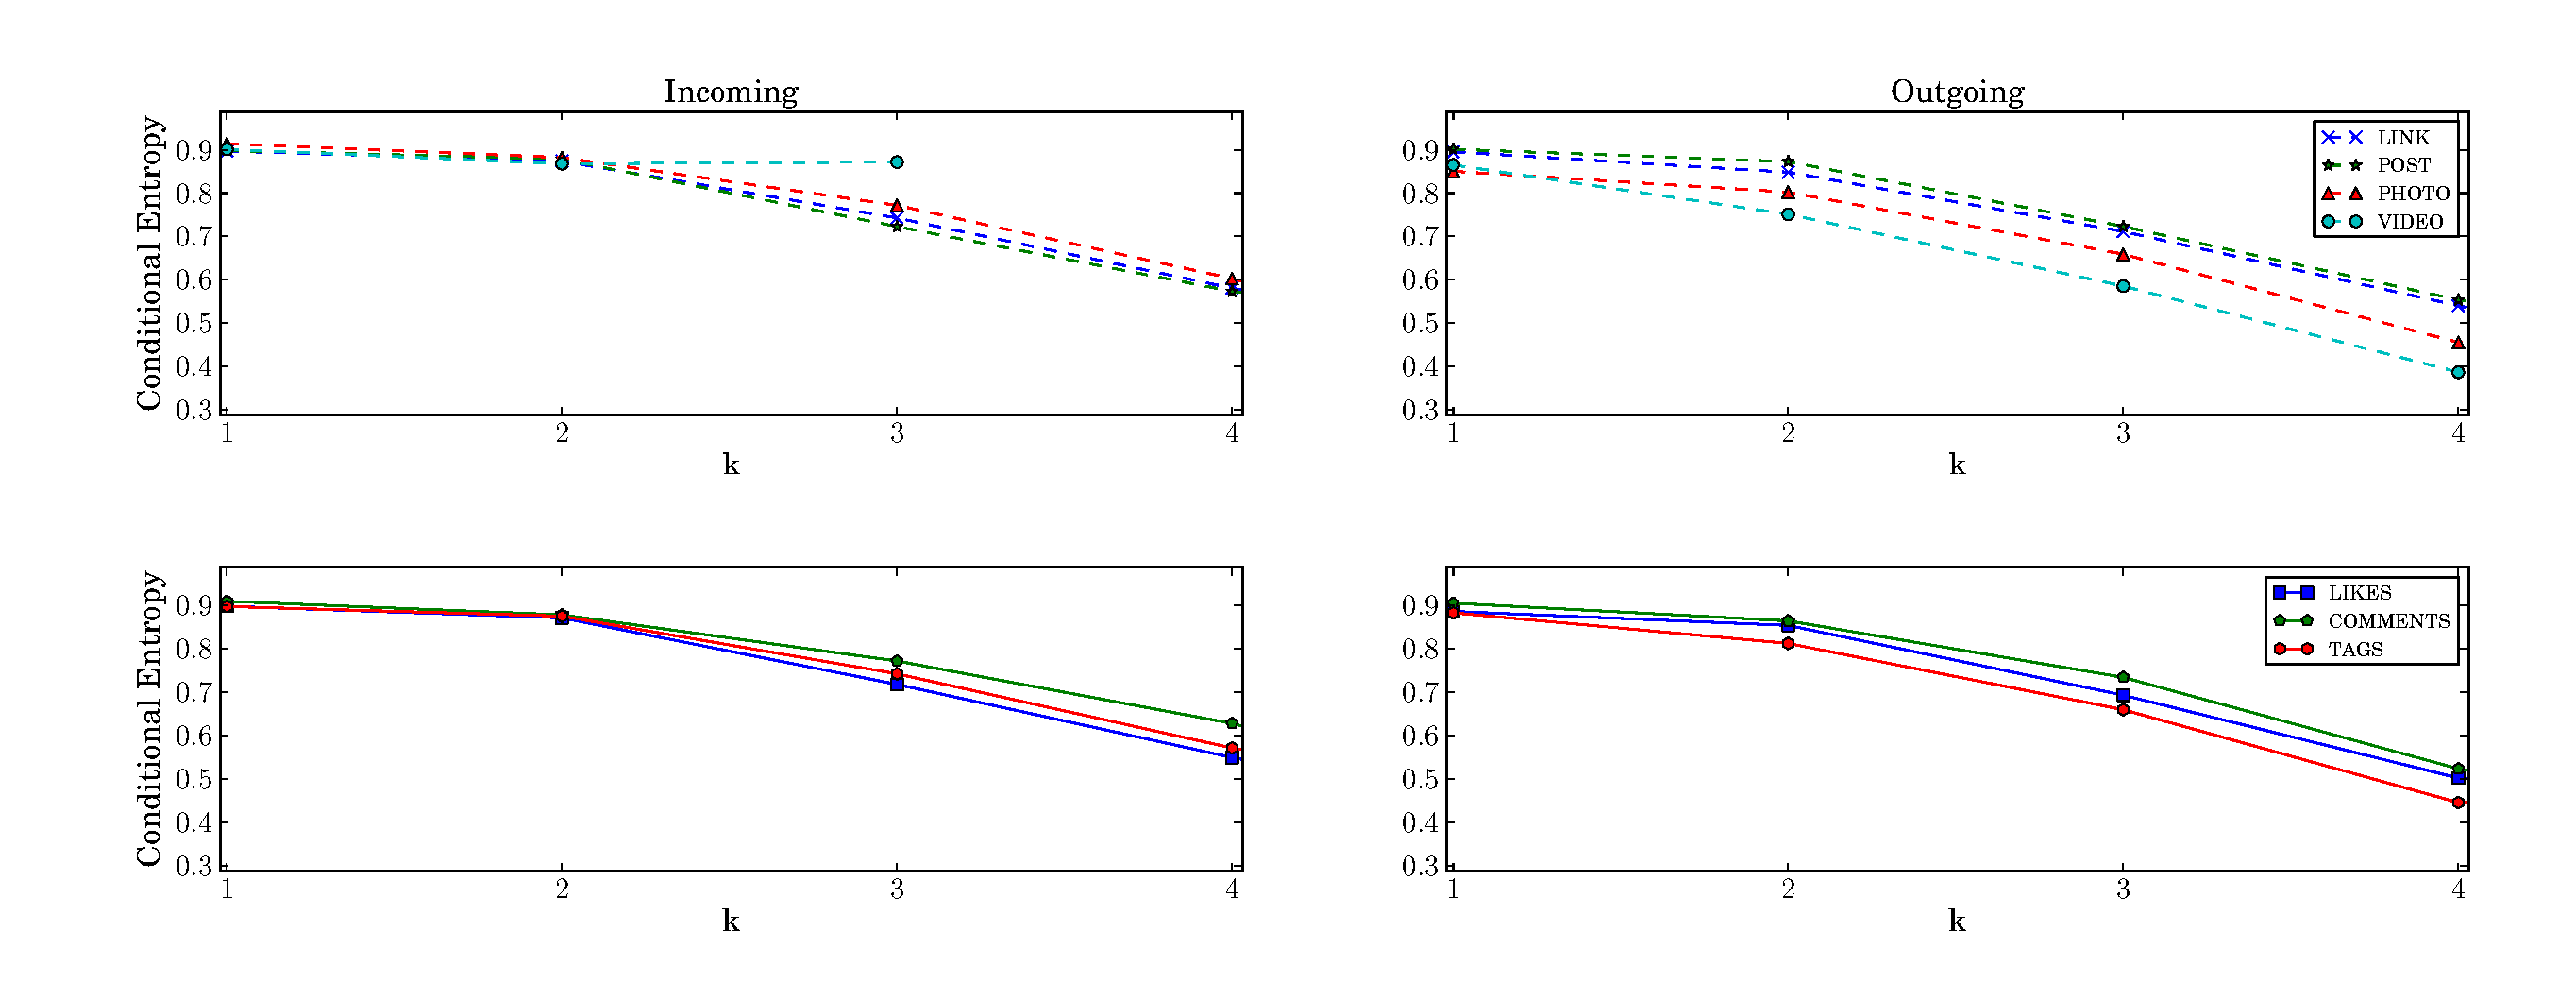
\includegraphics[width=210mm]{data/plots/vsk/ModalityActionsvsKFriends.eps}
\caption{Conditional Entropy  of modalities/activities for incoming/outgoing interactions vs item liked by at least k friends}
\label{Fig2}
\end{figure*}
%%%%%%%%%%%%%%%%%%%%%%%%%%%%%%%%%%%%%%%%%%%%%%%%%%%%%%%%%%%%%%%%%%%%%%%%%%%

\section{Interaction Analysis}

In this section we analyze the informativeness of Interaction SAGS,
namely those SAGs that are built w.r.t. a user $u$'s interactions.
A general method for measuring the amount of information that a 
feature $X$ provides w.r.t. predicting another variable $Y$ (in this
case likes or dislikes) is to calculate its conditional entropy:
\begin{align*}
H(Y&|X=True)\\
& = -\sum_{y\in{(\like,\dislike)}} p(y|X=true) \ln( p(y|X=true))
\end{align*}
In general, a lower conditional entropy indicates a more informative
feature.

As defined in Sec~\ref{sec:methodology}, we have three distinctions for user
interactions: modality, action, and directionality.  First we analyze
various interactions individually and jointly to understand what
interactions define SAGs with a high social affinity for a user $u$'s
preferences.  To this end, we make a few observations from the
conditional entropy analysis of Table~\ref{table:ce_interaction}:
\begin{itemize}
\item Users seem to have a stronger preferential affinity with those
  they interact with on videos vs. other modalities.  This could be
  due to the fact that video viewing is time-consuming and users
  inherently only watch the videos of those whose preferences they
  often share.
\item Tagging has a slightly better conditional entropy than
  commenting and liking.% indicating that tagging.
\item A user is more likely to share preferences with someone who she
  initiates the interaction with (outgoing) vs. with someone who
  initiates the interaction with her (incoming).  As an extreme
  instance of this, we note that while outgoing photo and video
  interactions are most informative, it appears that incoming photo
  and video interactions are least informative.
\end{itemize}

In figure \ref{Fig2} we plot conditional entropy of modality and
action for incoming/outgoing interactions constrained to links
liked by at least $k$ friends in the SAG.  Figure \ref{Fig2} reiterates
many observations made above for various $k$.  In addition, we note that
%\begin{itemize}
%% NOTED ABOVE NOW
%  \item Some interactions are more predictive than other. For
%    eg. videos and photo interactions were found to be significantly
%    more predictive than post and link interactions. Similarly,
%    tagging action is often more predictive than commenting and
%    liking.
%  \item As noted by previous work~\cite{saez2011high}, we observe that
%    outgoing interactions are more predictive than incoming
%    interactions. Furthermore, the differentiation between
%    predictiveness modalities and actions is more pronounced in
%    outgoing interactions than in incoming interactions.
%  \item 
preference affinity with a SAG increases as more people in the SAG
like the item --- then the more likely a user is to like an item.
While incoming interactions were not as predictive as outgoing
interactions for the same $k$, we note that higher $k$ for an incoming
interaction can be more predictive than lower $k$ for an outgoing
interaction.  This exhibits repeated exposure properties of epidemic
models for social networks~\cite{Golub2010selectionbiase}.
%\end{itemize}




%\subsection{Activity Analysis}
%\label{sec:activity_analysis}

%%!TEX root = document.tex

% Note: activity SAGs can go beyond friends.

%In this section we evaluate the correlation between the conditional
%entropy and size of groups, pages and favourites.

Now we analyse the informativeness of Activity Social Affinity
Features (ASAFs) by looking at the correlation between the size and
type of groups, pages and favourites.

Fig \ref{Fig3} shows the relationship between both the conditional
    entropy and logistic regression weights vs. the size of activity
    groups. Here the size of a {\em group}, {\em page} and {\em favourite} 
    is the number of total users in the activity group. 
    For {\em pages} and {\em pavorites} this is the total number of Facebook users, 
    whether or not they are in the App users' ego network, while for 
    {\em groups} only the number of users in the App users' ego network is visible to our app.
    Both scatter plots shows that the activity groups of small size can be
    highly predictive (low conditional entropy or weights that deviate
    extremely from zero) whereas large groups are rarely predictive.

In Fig~\ref{Fig4} we plot the average conditional entropy of the top
    10\% of features cumulative up to the size of the activity group given on the
    x-axis; this allows us to determine the marginal contribution of
    larger groups to the average conditional entropy as larger groups
    are incrementally added in.  This graph 
    distinctly shows that the small sizes of groups, pages and favourites
    have low average conditional entropy that transitions sharply to a
    higher average once a size threshold has been met.  From 
    Fig~\ref{Fig4} we can infer that the group sizes up to 50 and
    page/favourite sizes up to $10^{5}$ are most predictive.

%{\bf TODO: make this consistent with earlier discussion regarding persistence,
%temporally sychronized.}

 We also analyse predictiveness of favourites by categories in
    Fig~\ref{Fig5}, where the favorite category labels are obtained from the Facebook API.  
    %It shows that SAGs consisting of shared interests,
    %activity, television, and books are on average most predictive, while 
    %music, movies, favourite teams, sports and athletes are on average
    %least predictive.  
    We can see that contents in the ``long-tail'', i.e.,  
    having a large number of occurrences far from the most popular choices, 
    tend to have some of the most predictive indidividual affinities. Examples of these include
    music, books, movies. On the contrary, generic affinities (e.g. interests) and 
    those with a smaller number of choices (e.g. sports or fav-teams) 
    tend to be less predictive since they represent less specialised interests than 
    the long tail of music, book, or movie preferences.  

    These observations of Fig~\ref{Fig5} are also reiterated by the
    examples provided in Table~\ref{table:fav_examples} where uninformative favourites
    tend to have a broad appeal whereas informative favourites generally appear much
    more specialised.  This also reinforces the point that not all SAGs are predictive,
    but some are very predictive and it is important to learn which SAGs are informative
    rather than nai\"{v}ly aggregate their content, where on average, the features are
    clearly not informative.
   
    %#suvash#
    In Fig~\ref{fig:AccuracyVsactiveFeats} we analyse the relationship between accuracy and
    number of active features i.e. features that are true. We can see that accuracy increase as number of
    active features increases but then starts to decrese sharply. This may be due to the fact that items
    with large number of active features are likely to be general items, liked by wide variety of users,
    which makes it hard for SAF to make personalised prediction. 
    %While favourite teams, sports and athletes may be
    %too focused to offer much predictiveness vs. the other more diverse
    %categories, it is interesting that movies and music favourites
    %are not very predictive on average.  This may have to do with the fact that
    %these are typically ephemeral favourites that may be heavily influenced
    %by popularity as opposed to true personal preference.
%\end{itemize}

%In Fig~\ref{Fig4} we plot the average conditional entropy of top
%    10\% features cumulative over the size of activity group. It
%    distinctly shows that the small sized group, pages and favourites
%    have low average conditional entropy. Furthermore, it explains
%    average conditional entropy decreases as size increases. From the
%    figure \ref{Fig4} we can infer that the group size upto 50 and
%    page/favourite size upto $10^{5}$ can be highly predictive.
%
%We also analyze predictiveness of favourites by categories in
%    Fig \ref{Fig5}. It shows that television, books, music and movies
%    are predictive whereas favourite teams, sports and athletes are
%    less predictive.
%\end{itemize}

%\TODO{add a table of top 5-10 groups/pages/favs}

\begin{table*}[t!] \centering 

{\small
\begin{tabular}{|c|c|c|c|c|}
\hline 
\multicolumn{5}{|c|}{\textbf{Median Informative Favourites by Category}}\\
\hline 
\textbf{Books} & \textbf{Movies} & \textbf{Music} & \textbf{Television} & \textbf{Interests} \\
\hline \hline
Harry Potter series&Forrest Gump&John Lennon&Futurama&Travel\\
\hline
A Song of Ice and Fire&Pretty Woman&U2&Star Trek&Music\\
\hline
Discworld&Napoleon Dynamite&AC/DC&The Trap Door&Literature\\
\hline
Hitchhiker's Guide To The Galaxy&Harry Potter&The Smashing Pumpkins&Drawn Together&Painting\\
\hline
The Hobbit&Toy Story 3&Gotye&Sherlock(Official)&Running\\
\hline
The Magician's Guild&The Godfather&The Rolling Stones&Hitchhiker's Guide to the Galaxy&Sports\\
\hline
Ranger's Apprentice&Mulan&All Axess&Buffy The Vampire Slayer&Films\\
\hline
Cosmos&How to Train Your Dragon&Steve Aoki&South Park&Genetics\\
\hline
Foundation and Earth&The Princess Bride&Rihanna&24&Travelling\\
\hline
Deception Point&Watchmen&Billy Joel&The Daily Show&Internet\\
\hline
%5 point someone&Black Swan&Queens of the Stone Age&Monty Python's Flying Circus&Psychology\\
%\hline
%Freakonomics&Inception&Depeche Mode&Top Chef&Math\\
%\hline
%Alex Rider Series&Donnie Darko&Oasis&The Inbetweeners&Lambda\\
%\hline
%The Elenium&Kung Fu Panda&Justice&Firefly&Computer Science\\
%\hline
%Watchmen&American Psycho&Gorillaz&Red Dwarf&Skepticism\\
%\hline
\multicolumn{5}{c}{}\\
\hline 
\multicolumn{5}{|c|}{\textbf{Most Informative Favourites by Category}}\\
\hline
\textbf{Books} & \textbf{Movies} & \textbf{Music} & \textbf{Television} & \textbf{Interests} \\
\hline \hline
Calvin and Hobbes & Billy Madison & Avascular Necrosis & Metalocalypse & Computers\\
\hline
Tomorrow when the War Began & Team America: World Police & Tortured & Beast Wars & Texas HoldEm \\
\hline
I really like ceilings  & Pan's Labyrinth & Elysian & Hey Arnold! & Programming\\
\hline
Angels and demons  & Pirates of the Caribbean & Anno Domini & Sherlock & Economics\\
\hline
Magician  & Aladdin & Darker Half & Hey Hey It's Saturday & Martial arts\\
\hline
Digital Fortress  & Starship Troopers & Hellbringer & Neil Buchanan and Art Attack! & Graphic design\\
\hline
The Bible  & Happy Gilmore & Johnny Roadkill & Breaking Bad & Cooking\\
\hline
Interview with the Vampire  & Timon and Pumbaa & Aeon of Horus & Red vs. Blue & Klingon language\\
\hline
The Discworld Series  & Ferris Buellers Day Off & Katabasis & Stargate Universe & Politics\\
\hline
The Da Vinci Code  & Peter Griffin & Bane Of Isildur & Chaser's War on Everything & Science\\
\hline
\end{tabular}}
\caption{(top) Examples of 10 items per Favourite category near the \emph{median} conditional entropy (\emph{median informativeness}).
(bottom) Examples of top 10 items with the lowest conditional entropy (\emph{most informative}).
A general trend is that more informative favourite category ASAGs tend to be more specialised in
appeal, e.g. ``Avascular Necrosis'' is an informative music group favourite --- its members
tend to share common preferences --- while ``John Lennon'' and ``U2'' have a broader audience with
more diverse preferences. 
%#suvash#
Interestingly, ''Sherlock''  appears in both most and median informative table but the median informative is
an official page with wide range of fans, whereas the most informative is a duplicate fan page with few number of fans.}
\label{table:fav_examples}
\end{table*}

\eat{
\begin{table*}[tbp!]
\centering
\begin{tabular}{| >{\small}l | >{\small}r | >{\small}r |}
\hline
\textbf{Top Groups} & \textbf{Top Pages} & \textbf{Top Favourites} \\
\hline
%Heavy Metal - Australian Capital Territory & Avascular Necrosis & Avascular Necrosis \\
Heavy Metal - (city name) & Avascular Necrosis & Avascular Necrosis \\
Stephen Conroy Should Not Filter Our Internet & Assidian & Tortured \\
Silicone Stripper & Tortured & Elysian \\
Hardcore dancing is not moshing & Elysian & Anno Domini \\
%Metal bands come to Canberra cause I'm sick of... & Darker Half & Hellbringer \\
Metal bands come to (city name) cause I'm sick of... & Darker Half & Hellbringer \\
%Canberra Rock Gigs & Johnny Roadkill & Johnny Roadkill \\
(city name) Rock Gigs & Johnny Roadkill & Johnny Roadkill \\
%Let's Mosh - Canberra metal radio show - 2XX 9 & Anno Domini & Darker Half \\
Let's Mosh - (city name) metal radio show - 2XX 9 & Anno Domini & Darker Half \\
Bring Steel Panther to Australia & Billy Madison & Bane Of Isildur \\
%Canberra Death/Heavy Metal Appreciation & Hellbringer & Katabasis \\
(city name)  Death/Heavy Metal Appreciation & Hellbringer & Katabasis \\
Robert The Bruce (Band) & Metalocalypse & Aeon of Horus \\
\hline
\end{tabular}
\caption{Top 10 Groups/Pages/Favourites ranked by Conditional Entropy. The city name where our institution and many Facebook users resides is anonymized.}
\label {table:topGroupPagesFavs}
\end{table*}}

%%%%%%%%%%%%%%%%%%%%%%%%%%%%%%%%%%%%%%%%%%%%%%%%%%%%%%%%%%%%%%%%%%%%%%%%%%%
\begin{figure*}[tbp!]
\centering
\begin{tabular}{ccc}
\begin{tabular}{ccc}
\subfloat[Fig:][]{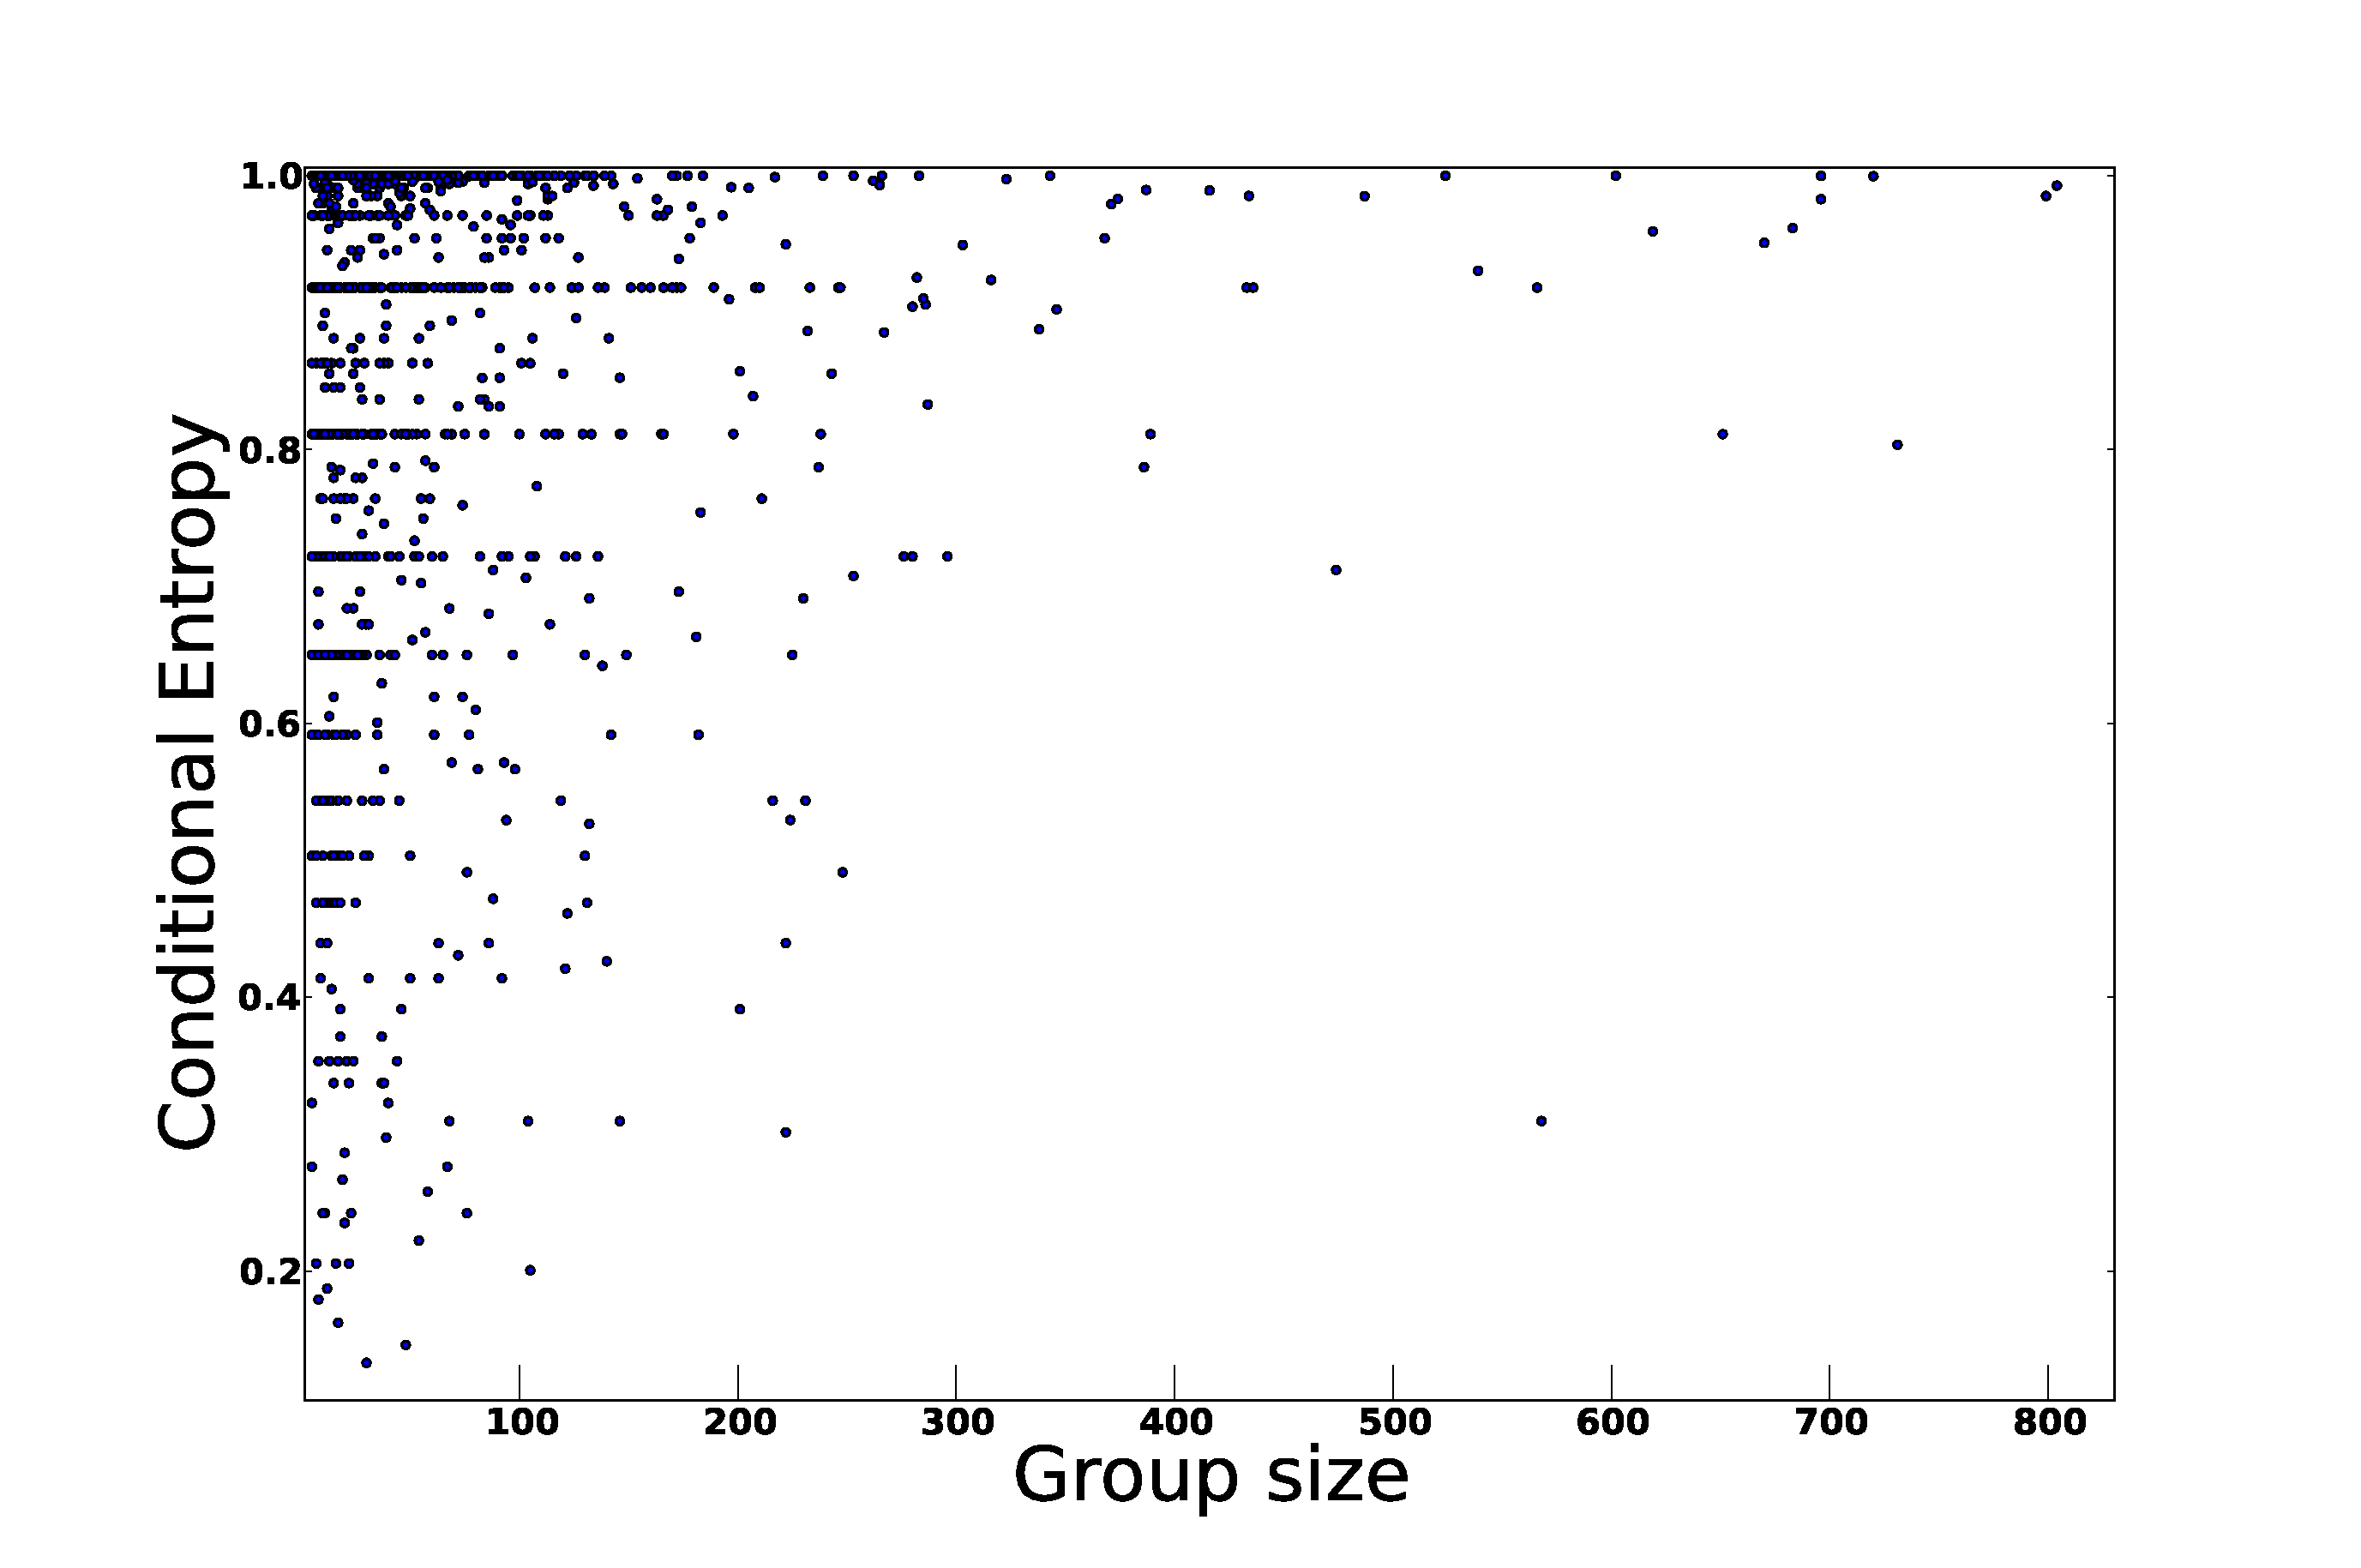
\includegraphics[width=45mm, height=35mm]{data/plots/new/CEvsGroupSize.eps}}
\subfloat[Fig:][]{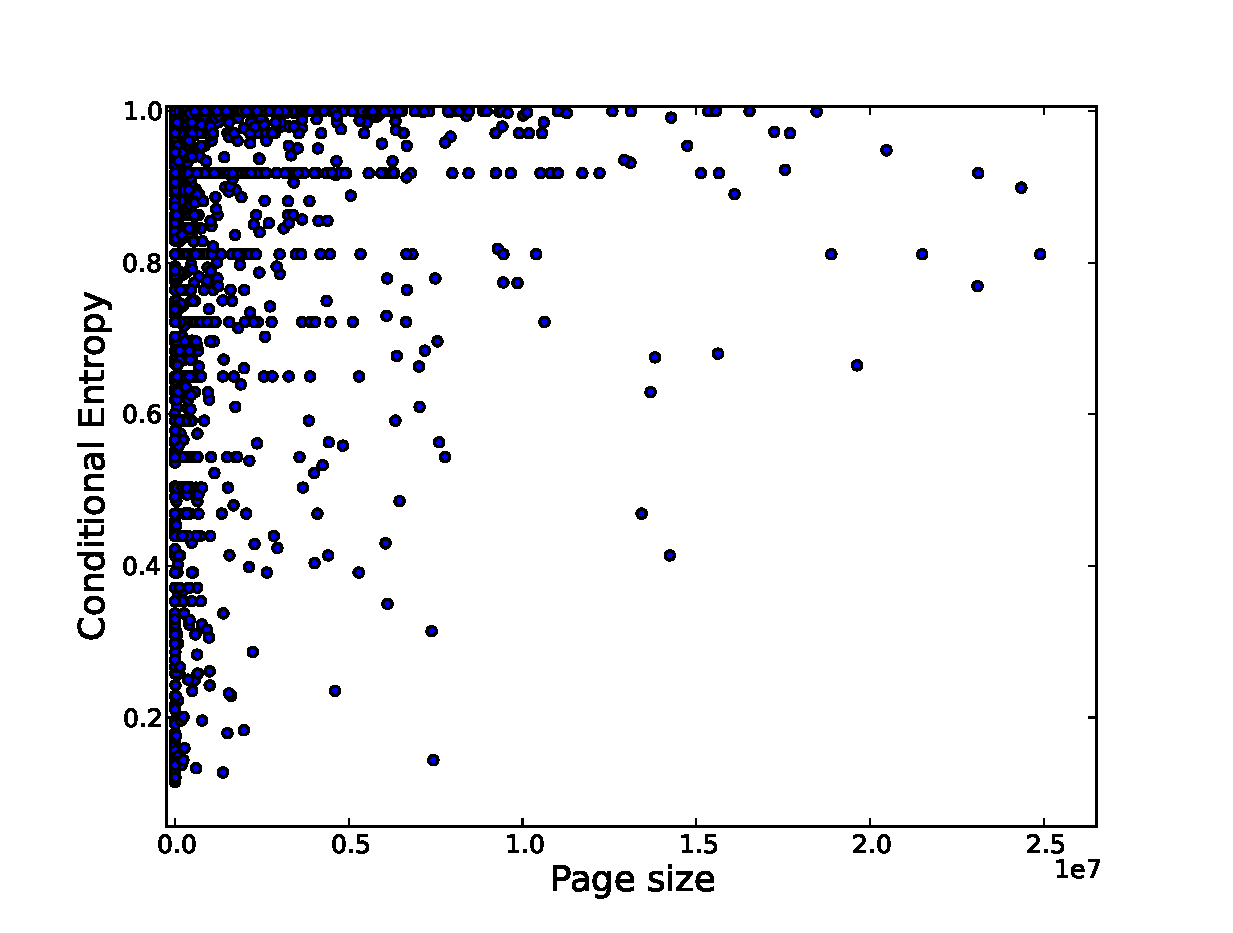
\includegraphics[width=45mm, height=35mm]{data/plots/new/CEvsPageSize.eps}}
\subfloat[Fig:][]{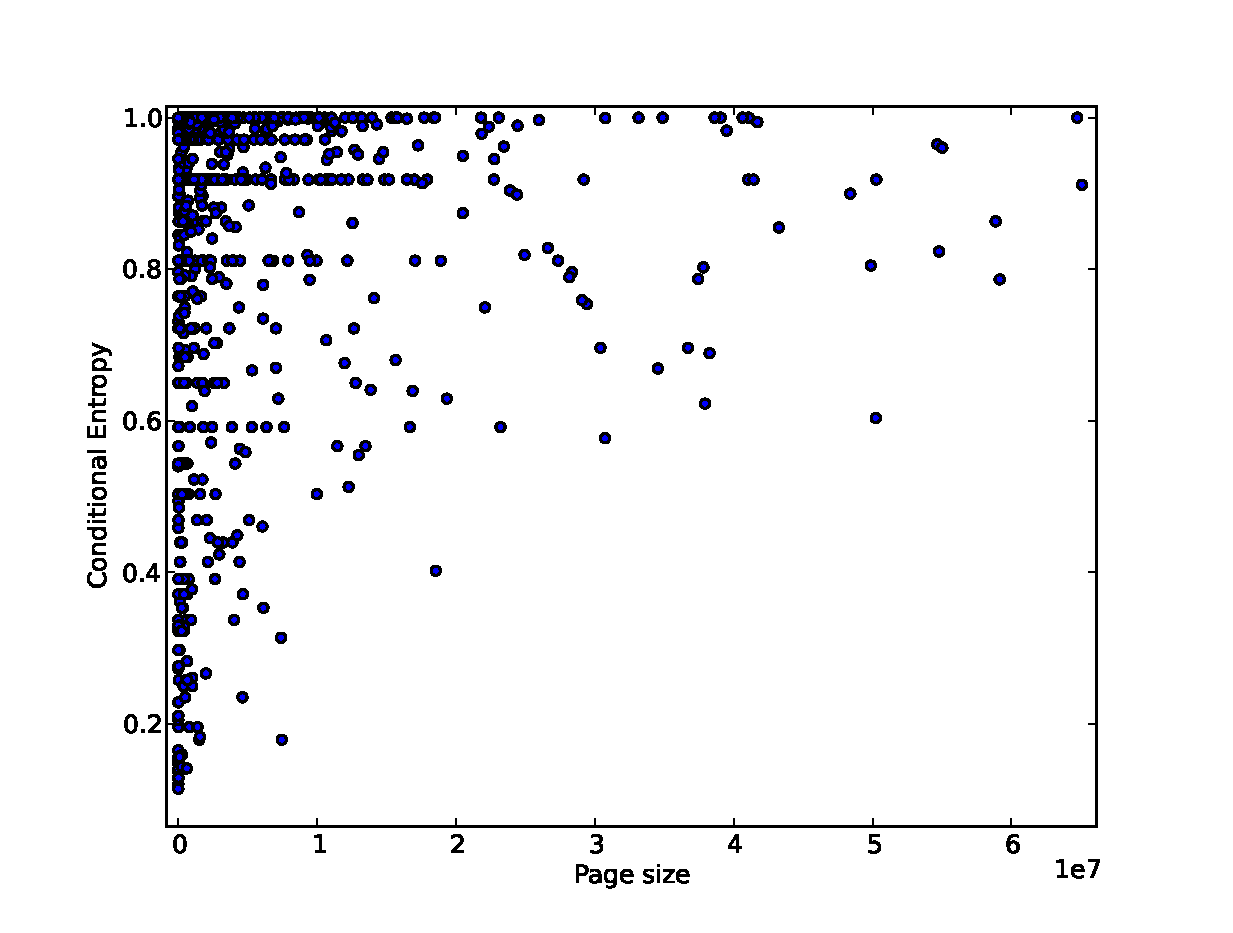
\includegraphics[width=45mm, height=35mm]{data/plots/new/CEvsFavSize.eps}} \\
%\vspace{-10mm}
\subfloat[Fig:][]{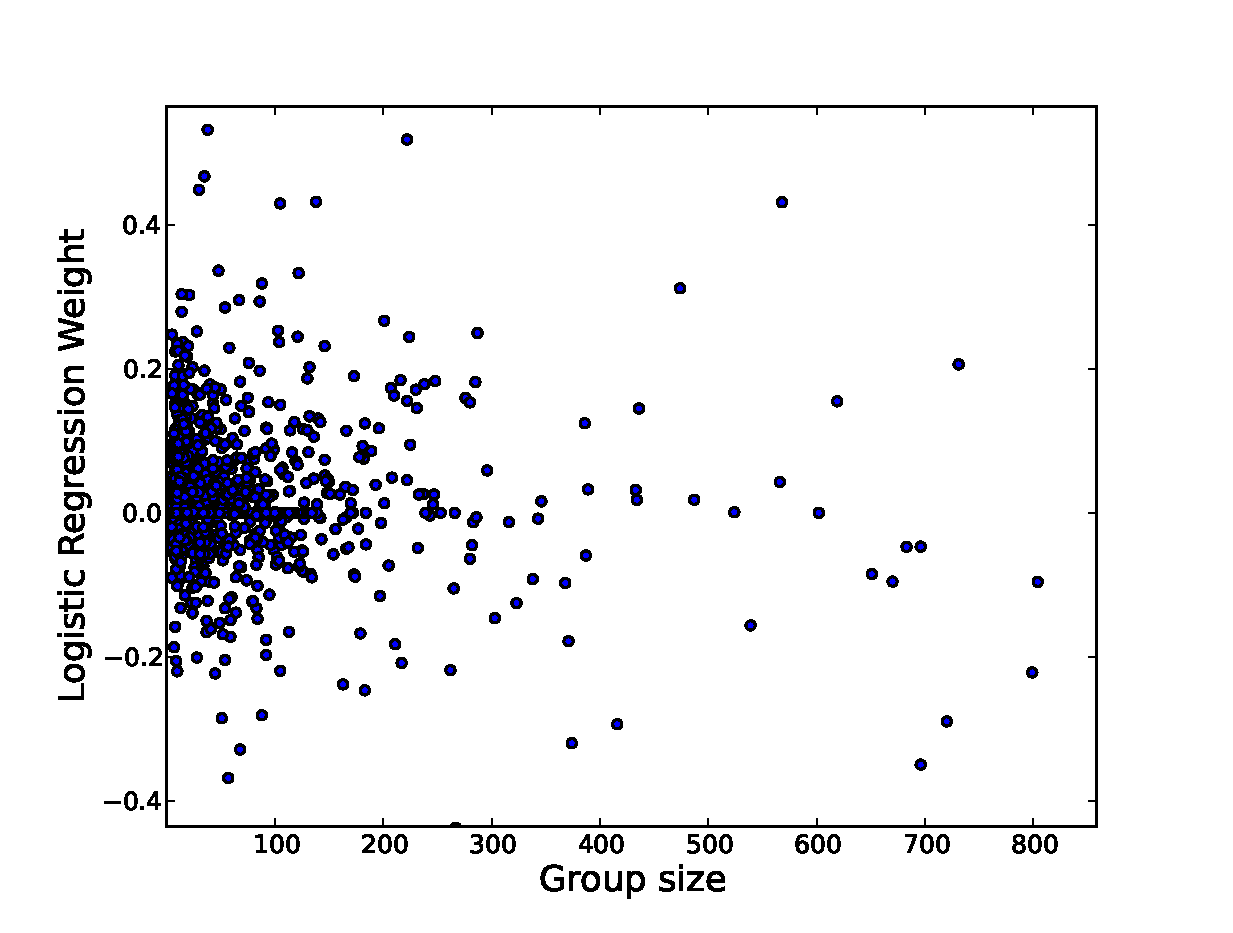
\includegraphics[width=45mm, height=35mm]{data/plots/new/LRweightvsGroupSize.eps}}
\subfloat[Fig:][]{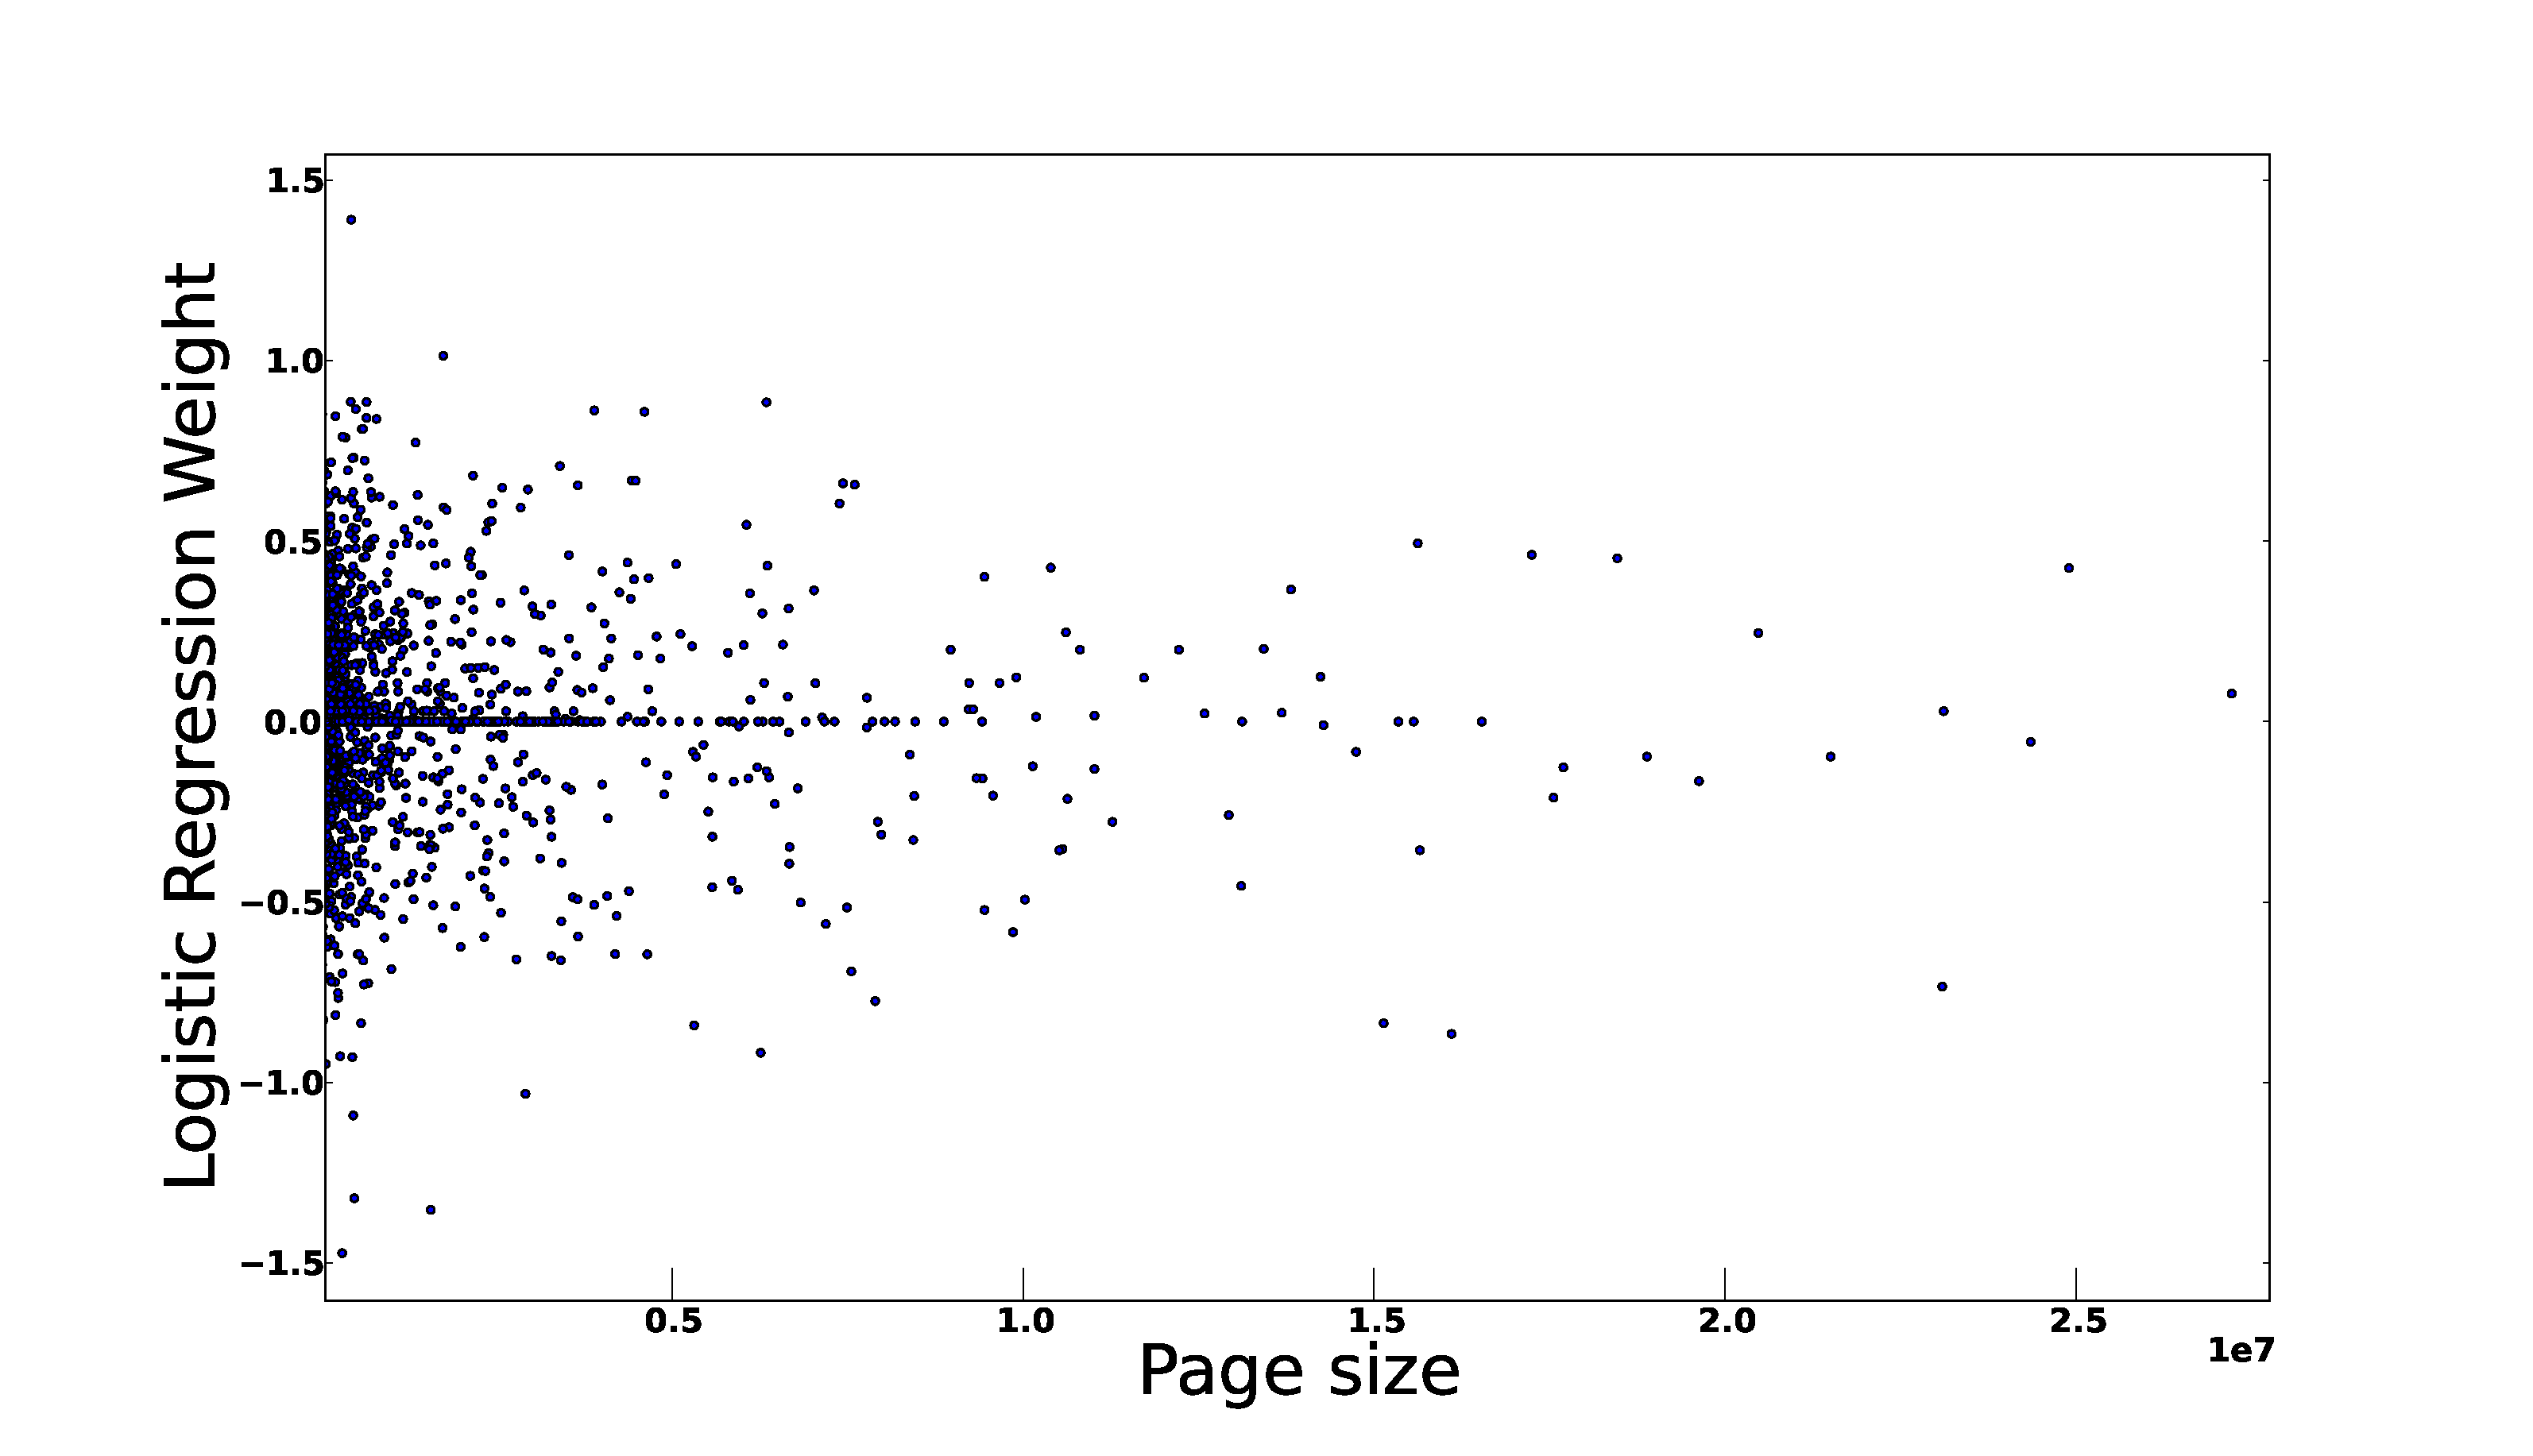
\includegraphics[width=45mm, height=35mm]{data/plots/new/LRweightvsPageSize.eps}}
\subfloat[Fig:][]{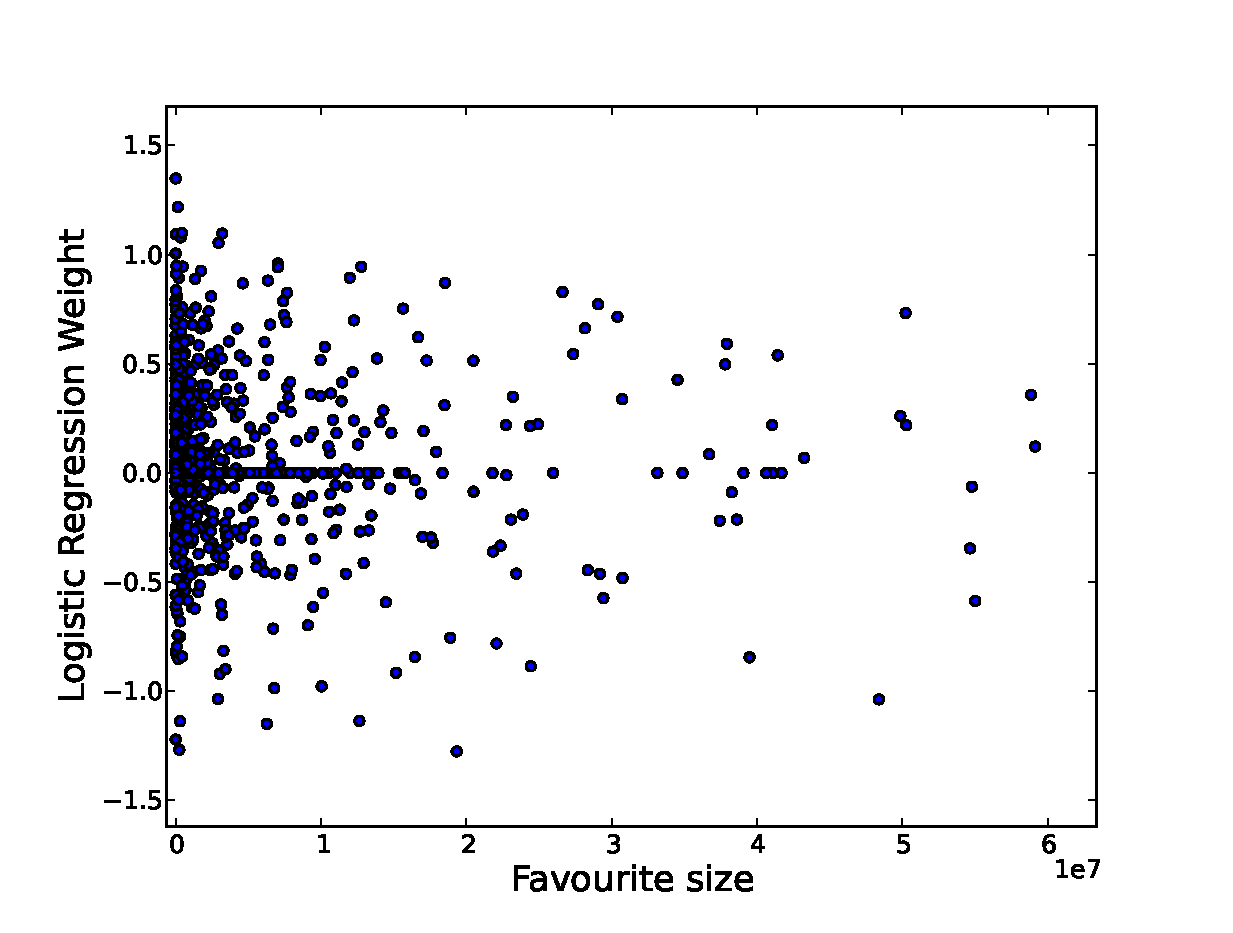
\includegraphics[width=45mm, height=35mm]{data/plots/new/LRweightvsFavSize.eps}} \\
\end{tabular}
\end{tabular}
\vspace{-2mm}
\caption {Conditional entropy vs size (a-c); logistic regression feature weights vs size (d-f).
In (a-c) we observe that the large membership ASAGs are rarely informative while the most
informative SAGs tend to have low memberships.  Similarly in (d-f) we see that the most
predictive features with the most extreme weights are concentrated toward small ASAGs. }
\label{Fig3}
\end{figure*}
%%%%%%%%%%%%%%%%%%%%%%%%%%%%%%%%%%%%%%%%%%%%%%%%%%%%%%%%%%%%%%%%%%%%%%%%%%%

%\vspace{-5mm}

%%%%%%%%%%%%%%%%%%%%%%%%%%%%%%%%%%%%%%%%%%%%%%%%%%%%%%%%%%%%%%%%%%%%%%%%%%%
\begin{figure*}[tbp!]
\centering
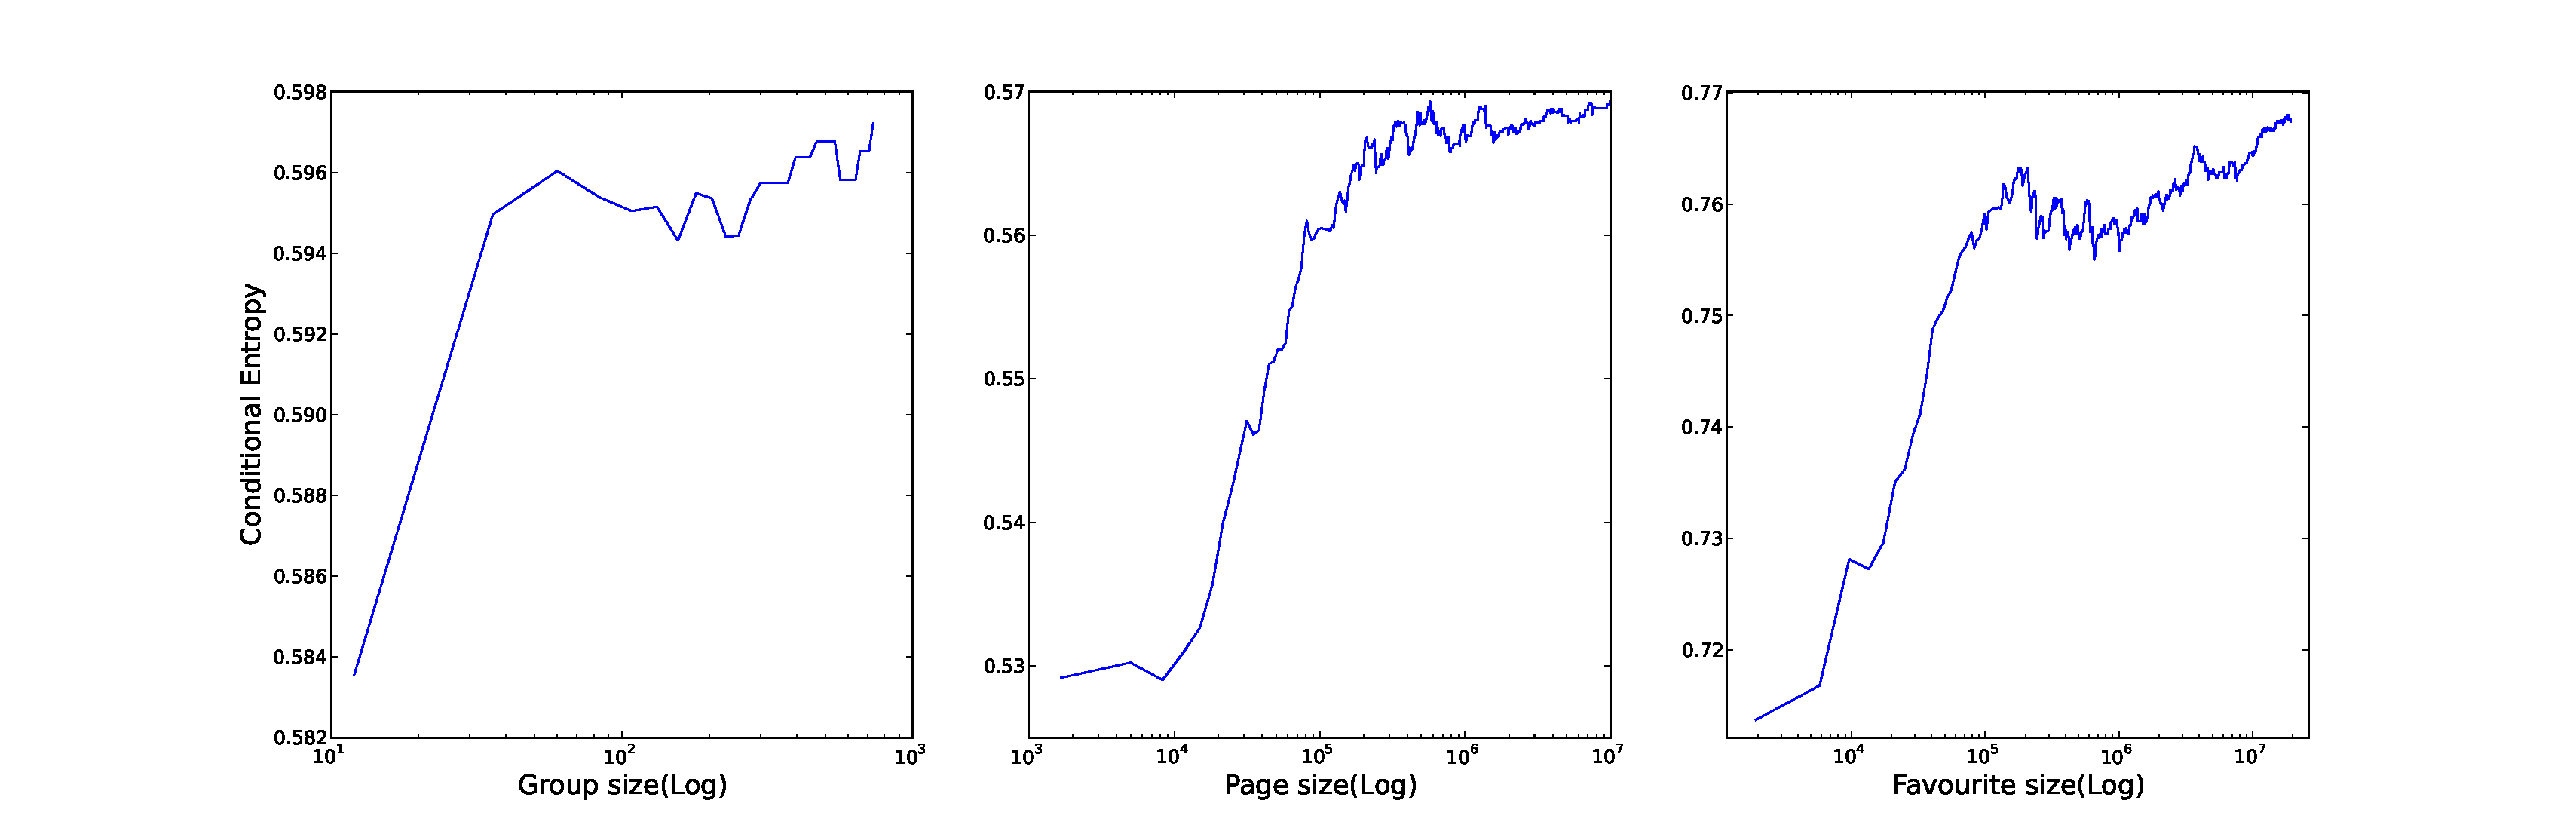
\includegraphics[scale=0.28]{data/plots/cumulativeEntropy/cumulative.eps}
\vspace{-3mm}
\caption{Average conditional entropy of top 10\% groups, pages and favourite features \emph{cumulative} over the size.  Here we see that as we add in larger membership ASAGs, the average informativeness
decreases substantially (entropy increases).}
\label{Fig4}
\end{figure*}
%%%%%%%%%%%%%%%%%%%%%%%%%%%%%%%%%%%%%%%%%%%%%%%%%%%%%%%%%%%%%%%%%%%%%%%%%%%

%\vspace{-7mm}

%%%%%%%%%%%%%%%%%%%%%%%%%%%%%%%%%%%%%%%%%%%%%%%%%%%%%%%%%%%%%%%%%%%%%%%%%%%
\begin{figure*}[tbp!]
\hspace{-12mm}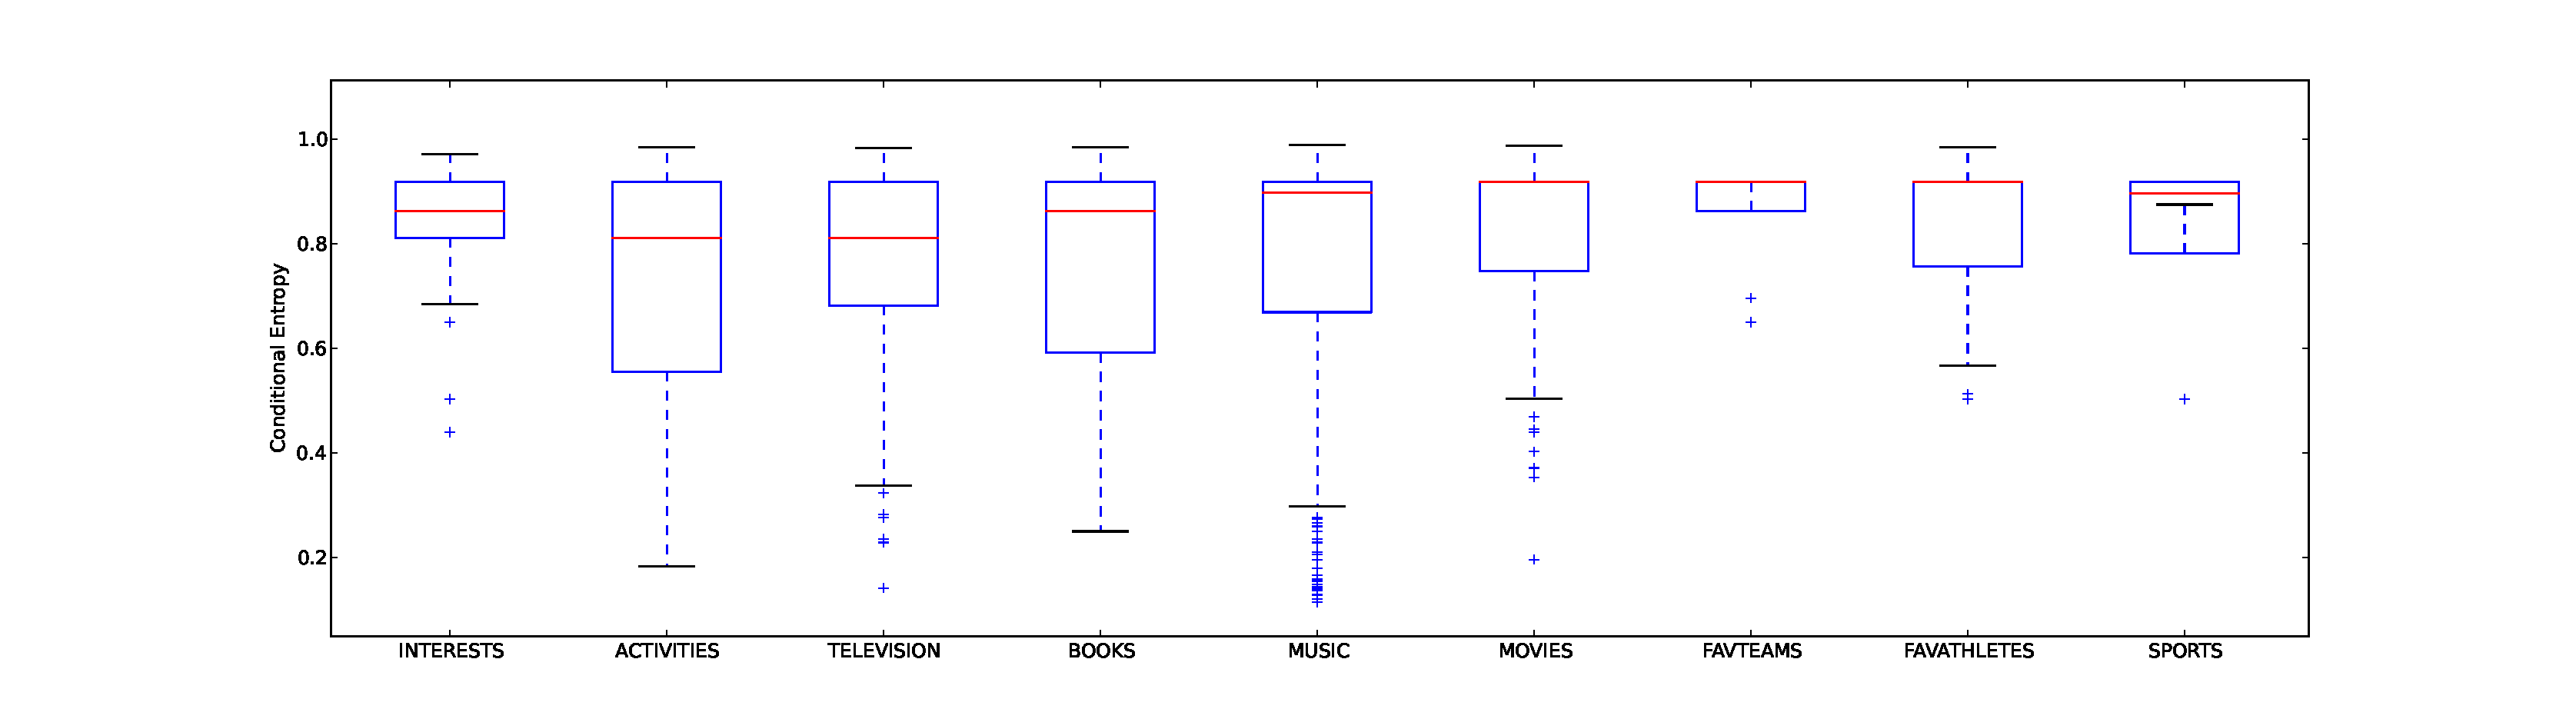
\includegraphics[width=200mm]{data/plots/boxPlots/CEvsFavTypes.eps}
\vspace{-7mm}
\caption{Conditional entropy for top 1000 favourites breakdown by categories.  While ASAG categories
with many options like music are not informative on average, we see
that some of the most informative ASAGs are music.  This reiterates
the point that it is crucial to \emph{learn} which ASAGs (or ISAGs)
are informative rather than aggregating average information.}
\label{Fig5}
\end{figure*}
%%%%%%%%%%%%%%%%%%%%%%%%%%%%%%%%%%%%%%%%%%%%%%%%%%%%%%%%%%%%%%%%%%%%%%%%%%%

%#suvash#
\begin{figure*}[tbp!]
\centering
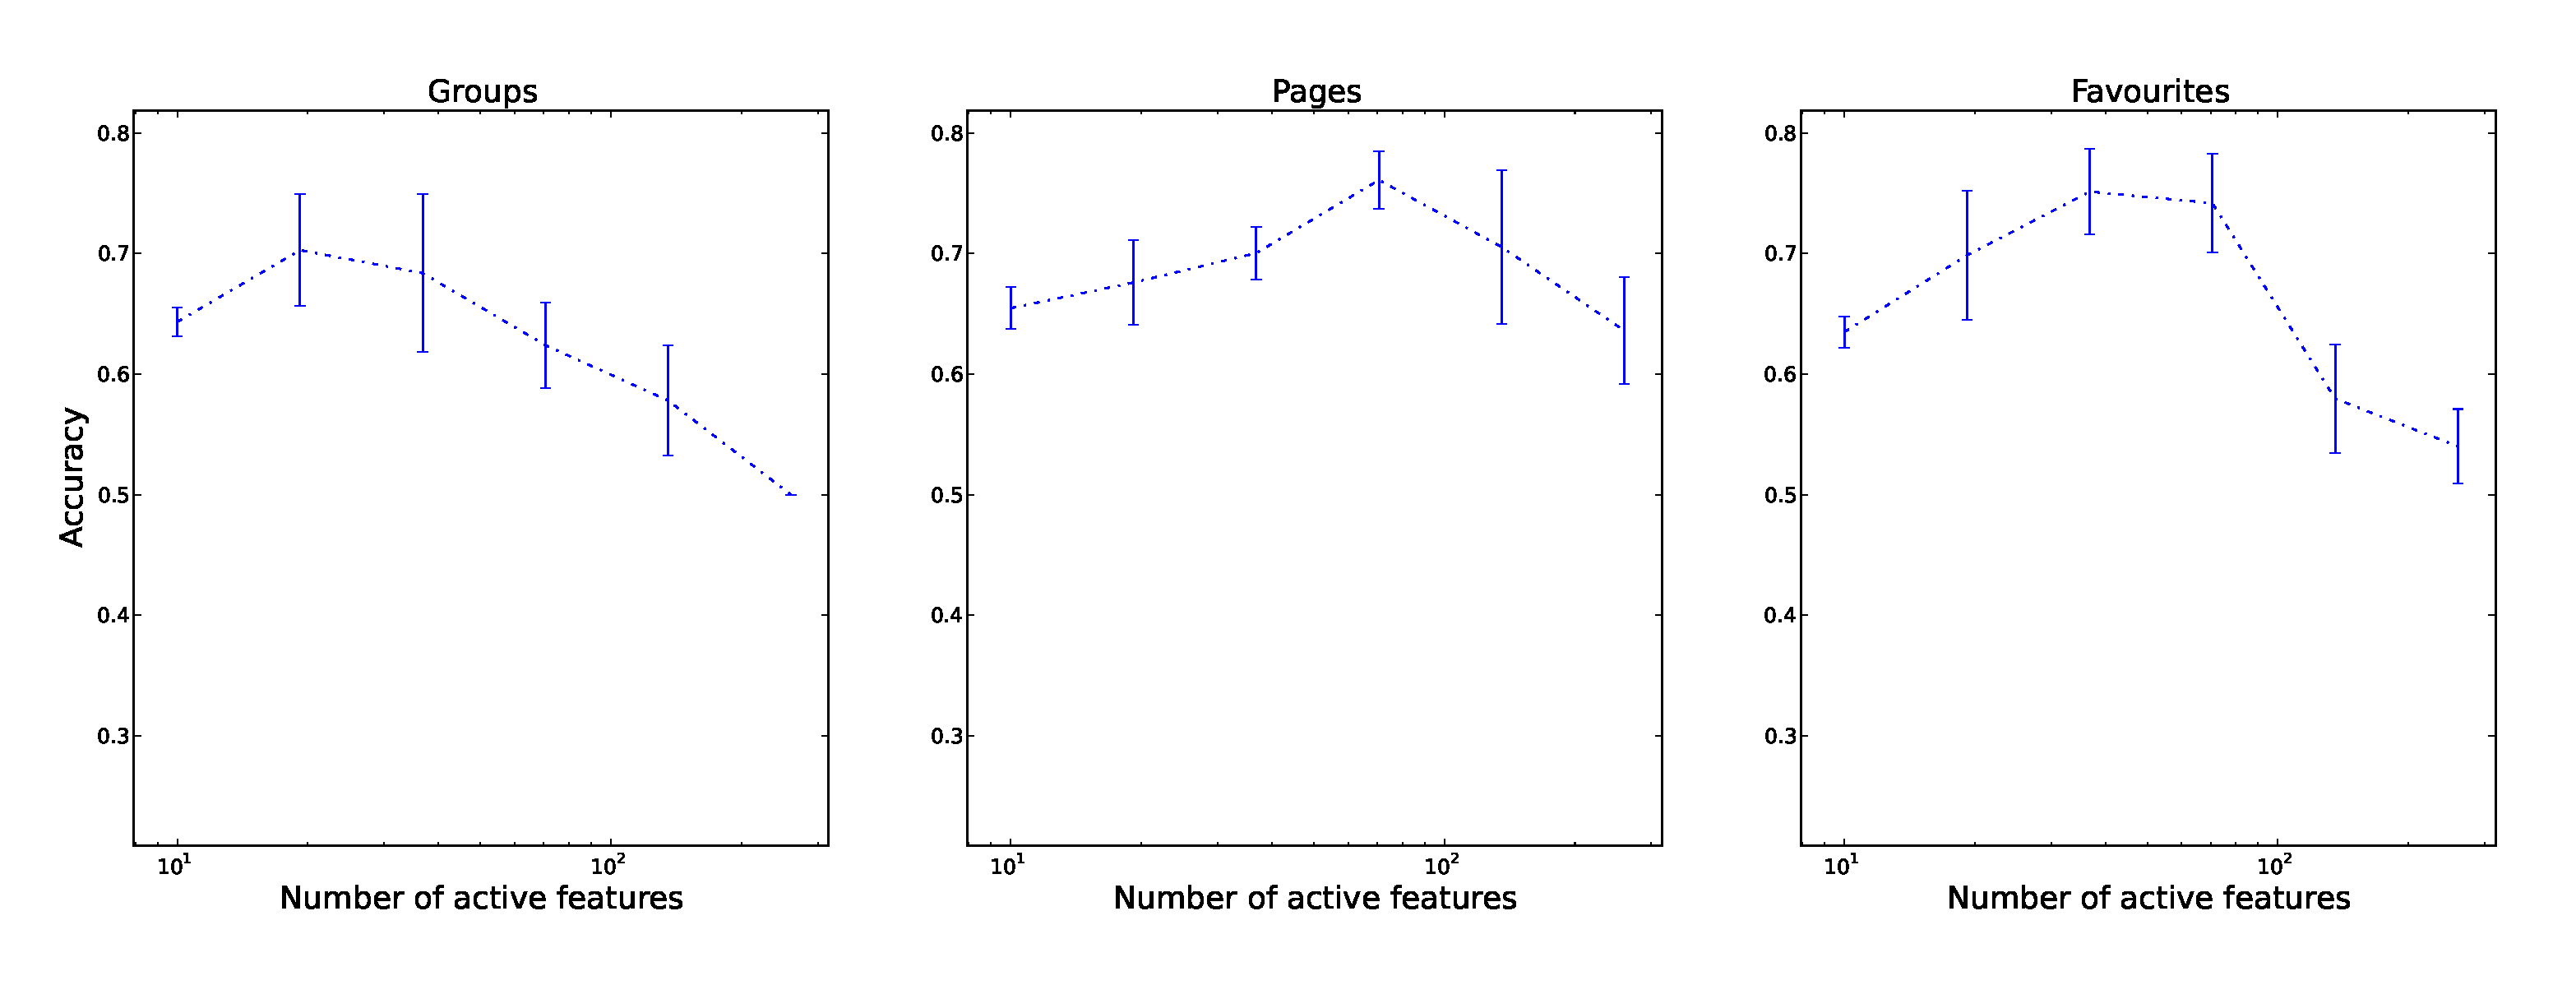
\includegraphics[width=180mm, height=60mm]{data/plots/new/accuracyVsactiveFeatures.eps}
\vspace{-3mm}
\caption{Accuracy increases as the number of active features increases, but then, after reaching a certain limit, it starts to decrease sharply.
}
\label{fig:AccuracyVsactiveFeats}
\end{figure*}



\section{Related Work}

%!TEX root = document.tex

%{\bf TODO: some related work is ``eaten'' in the intro and methodology, should it be inserted here?}

%There has been many recent work on inferring user preferences on information 
 
This work relates to many others in inferring user preferences on social and information networks. 
We structure the discussion into three parts: the first is concerned with the nature of user traits, interactions and diffusion, the second is concerned with relating these user traits and interactions to user preferences, interests and the strength of social ties.

%% No longer fits cleanly in the intro, should be moved into related
%% work is not already mentioned there.  -SPS
\TODO{
In the context of recent work on social
recommendation~\cite{sorec,ste,lla} and information diffusion
~\cite{Goel2012structure,Romero2011hashtag,Bakshy2012chamber}, it is
important to know which of these interactions or common traits are
actually reflective of common preferences.
%% This is good text, but probably better in related work.  We have CIKM reviewers here who are
%% just skimming and trying to follow the technical setup in the initial sections... this
%% serves as a bit of a digression that detracts from some of the more important quantitative
%% points that we want to drive home with the reader as early as possible.  -SPS


Note that the notion of affinity we adopt is based on direct user {\em actions}, rather than
static profile information, or structural information of the social graph. 
We believe this is a useful view into the social network, as it was recently pointed out
that a user's attention (i.e., interactions) are divided among a small subset of Facebook friends~\cite{backstrom2011center}, and that ratings of real-world friendship strength seems to be more predictable from the intimacy, intensity, and duration of interactions, than from social distance and structural information~\cite{gilbert2009predicting}. Our affinity definition is based on direct interactions within a users' ego network, this is complementary to 
a recent alternative~\cite{Panigrahy2012ubr} that uses number of paths between two users encodes the resilience of network structure, 
as it was recently found~\cite{Goel2012structure} that the vast majority of information diffusion
happens within one step from the source node. 
}

%To structure the discussion, we categorize the observables into three types:
%There are three main types of observables in such networks 
%(1) {\em User profile} including friendship information, they change at a much slower rate than information propagation in the network; (2) a dynamic stream of {\em interactions}, between users or between a user and a digital object; (3) a global and networked view of interactions, i.e. {\em diffusion} cascades. There are two types of hidden information that are common targets of inference and prediction: (a) User {\em preference} and interest, sometimes expressed as positive and negative (e.g. likes, voting up or down) action; (b) the inherent strength of {\em social ties}. 
%While the main objective of our study is to correlate 
%interactions and profile to user preference, 

The first group studies the nature of user profile, interactions, and diffusion.
Profile information and demographics is correlated with user behavior
patterns. \cite{Chang2010ethnicity} showed that the tendency to
initiate a Facebook friendship differs quite widely across ethnical
groups, while \cite{backstrom2011center} have additionally showed that female and male users have opposite tendencies for dispersing attention for within-gender and across-gender communication.
Two particular measurement studies on Facebook attention~\cite{wilson2009user,backstrom2011center} have inspired our work.  Although the average number of friends for a Facebook user is close to the human psychological limit, known as the Dunbar number~\cite{hill2003social}, the findings concur that a user's attention (i.e., interactions) are divided among a much smaller subset of Facebook friends. \cite{backstrom2011center} studied two types of attention: communication interaction and viewing attention (e.g. looking at profiles or photos). Users' communication attention is focused on small numbers of friends, but viewing attention is dispersed across all friends.
This finding supports our approach of looking at many types of user interactions across all of a user's contact network, as a user's interest is driven by where he or she focuses attention on.

The mechanisms of diffusion invites interesting mathematical and empirical investigations. %of diffusion has generated many interesting observations. 
The Galton�Watson epidemics model suits the basic setup of social
message diffusion, and can explain real-world information cascade such as
email chain-letters when adjusted with selection
bias~\cite{Golub2010selectionbiase}. For social diffusions in a
one-to-many setting, however, the epidemics model has been less
accurate. \cite{ver2011stops} found that online message cascades (on
Digg social reader) are often smaller than prescribed by the epidemics
model, seemingly due to the diminishing returns of repeated
exposure. \cite{Romero2011hashtag}, in an independent study, confirmed
the effect of diminishing returns with Twitter hashtag cascades, and
further found that cascade dynamics differ across broad topic
categories such as politics, culture, or sports. Our observations on a number of Facebook interactions agrees with the effect of diminishing returns.

The nature of social diffusion seem to be not only democratic~\cite{asur2011trends,Bakshy2011everyone}, but also broadening for users~\cite{Bakshy2012chamber}. While influential users are important for cascade generation~\cite{Bakshy2011everyone}, large active groups of users are needed to contribute for the cascade to sustain~\cite{asur2011trends}. Moreover, word-of-mouth diffusion can only be harnessed reliably by targeting large numbers of potential influencers, confirmed by observations on Twitter~\cite{Bakshy2011everyone} and online ads~\cite{influence}. In a study facilitated by A/B testing on Facebook links, \cite{Bakshy2012chamber} found that while people are more likely to share the information they were exposed to by their strong ties than by their weak ties, the bulk of information we consume and share comes from people with different perspectives (weak ties). Our Facebook App is intended to bridge this gap between insights from these observations and predicting user actions.

The second group of related work tries to correlate from user interactions to preferences and tie strength. 
~\cite{saez2011high} found that incoming and outgoing actives are
highly correlated on broadcast platforms such as Facebook and Twitter,
and such correlation does not hold in one-to-one mode of communication
such as email. Multiple studies have found that online interactions
tend to correlate more with interests than with user profile. \cite{singla2008yes} found that user who frequently interact (via MSN chat) tend to share (web search) interests. 
\cite{Anderson2012} concluded that the level of user activities correlate with the positive ratings that they give each other, and it is less about what they say (content of posts) but more about who they interacted with. Such findings echo those by ~\cite{brandtzag2011facebook}
that real-world interactions further strengthens friendship on Facebook, while virtual interactions reveal interests. Furthermore, ratings of real-world friendship strength and trust~\cite{gilbert2009predicting} seems to be more predictable from the intimacy, intensity, and duration of interactions, than from social distance and structural information. 
In terms of making the interaction-to-preference operational, \cite{nori2011exploiting} examines the predictability of user actions on Twitter from actions in both Twitter and Del.icio.us. The study uses both linear regression and an bipartite graph model that outperformed state-of-the-art models. ~\cite{gomes2011social} derived rules for Facebook interactions using a psychology-inspired formal symbolic language. 
These work are most closely related to ours, yet none has examined such a diverse set of user actions in the same context: one-on-one interactions (e.g. commenting), broadcast (e.g. posting, sharing), and co-preference (e.g. likes). 
%From data mining these rules, ranking them on confidence and support, the study found users are more likely to `like' another user's post or comment than to actively comment on it, and that the action of a `like' or `comment' by one user does not affect the involvement of other users in social interactions.

In summary, our study is motivated by overall utility of weak ties, diverse, and very specific interactions. To the best of our knowledge, this is the first work that look at all of various combinations of interactions and user traits outlined in our Methodology.  Our preliminary findings confirm many of the observations made in the literature while shedding new light on some of these effects (and new causes of these effects) for a rich set of Facebook user and interaction data.


\section{Conclusions}

\input conclusion

\bibliography{bibliography}
\bibliographystyle{abbrv}

\end{document}

